\documentclass[review]{elsarticle}

\usepackage{lineno,hyperref}

\usepackage{graphicx}% Include figure files
\usepackage{dcolumn}% Align table columns on decimal point
\usepackage{amsmath}
\usepackage{amssymb}
\usepackage{epstopdf}
\usepackage{multirow}
\usepackage{color}
%\usepackage{hepparticles} % particle names
%\usepackage{hepnames} % shortcuts for lots of particle names
\usepackage[alsoload=hep]{siunitx}
\sisetup{ per-mode=symbol}


\graphicspath{{figures/}}

\modulolinenumbers[5]

\journal{}
\bibliographystyle{elsarticle-num}


%%%%%%%%%%%%%%%%%%%%%%%%%%%%%%%%%%%%%%%%%%%% 
\newcommand*{\MIT }{Massachusetts Institute of Technology, Cambridge, Massachusetts 02139, USA}
\newcommand*{\ODU}{Old Dominion University, Norfolk, Virginia 23529}
\newcommand*{\JLAB}{Thomas Jefferson National Accelerator Facility, Newport News, Virginia 23606}
\newcommand*{\TAU }{School of Physics and Astronomy, Tel Aviv University, Tel Aviv 69978, Israel}
\newcommand*{\Penn}{Pennsylvania State University, University Park, PA, 16802}


\begin{document}


%%%%%%%%%%%%%%%%%%%%%%%%%%%%%%%%%%%%%%%%%%%%%%%%%%%%%%%%%%%%%%%%%%%%%%%%%%%%%%%%%%%%%%%%%%%%%%%%%%%
\begin{frontmatter}

\title{The CLAS12 Backward Angle Neutron Detector (BAND) for high momentum neutrons}

%% Group authors per affiliation:
\author{E.P.~Segarra, F.~Hauenstein, A.~Schmidt, R.~Cruz-Torres, \\O.~Hen, A.~Denniston, T.~Kutz, J.~Pybus\corref{mycorrespondingauthor}}
\address{\MIT}
\author{C.~Fogler, L.B.~Weinstein}
\address{\ODU}
\author{E.~Piasetzky}
\address{\TAU}
\author{K.~Pryce}
\address{Orsay}
\author{I.~Vega, M.~Mu\~nos}
\address{UTFSM}

%%%%%%%%%%%%%%%%%%%%%%%%%%%%%%%%%%%%%%%%%%%%%%%%%%%%%%%%%%%%%%%%%%%%%%%%%%%%%%%%%%%%%%%%%%%%%%%%%%%
\author[]{}
\ead[]{}

\begin{abstract}
The Backward Angle Neutron Detector (BAND) of CLAS12 is discussed. The detector is positioned $3$ \si{\meter} upstream of the target to 
detect backward neutrons with momenta between $0.25$ and $0.7$ \si{\GeV/\clight}. It consists of $18$ rows and $5$ layers of $7.2$ \si{\centi\meter} 
by $7.2$ \si{\centi\meter} scintillator bars with PMT readout on both ends to measure the neutron time-of-flight from the target and the 
energy deposition in the scintillator layers. There is an additional $1$ \si{\centi\meter} veto layer for vetoing charged particles. The detector 
covers an angular range of backward going particles from $155$\si{\degree} to $175$\si{\degree} with a detection efficiency of 
$35$\% and momentum resolution of $<1.5$\%.
\end{abstract}

\begin{keyword}
CLAS12; Time of flight; Plastic scintillator; Fast neutrons
\end{keyword}
\end{frontmatter}

%%%%%%%%%%%%%%%%%%%%%%%%%%%%%%%%%%%%%%%%%%%%%%%%%%%%%%%%%%%%%%%%%%%%%%%%%%%%%%%%%%%%%%%%%%%%%%%%%%%
\linenumbers

\section{Overview of CLAS12}


The CLAS12 (Cebaf Large Angle Spectrometer)[ADD REF] in Jefferson Lab's HallB experimental hall is a multi-purpose spectrometer to detect charged and neutral particles. It covers angles from xx to xx and momenta from xx to xx for the different particles. For our physics of interest, it is necessary to detect recoil neutrons with momenta above \SI{200/250}{\mega\eVperc} at backward angles. Therefore, a new detector has been build to detect these neutrons, the Backward Angle Neutron Detector (BAND); see Fig.~\ref{fig:clas12}.

\begin{figure}[h]
	\centering
	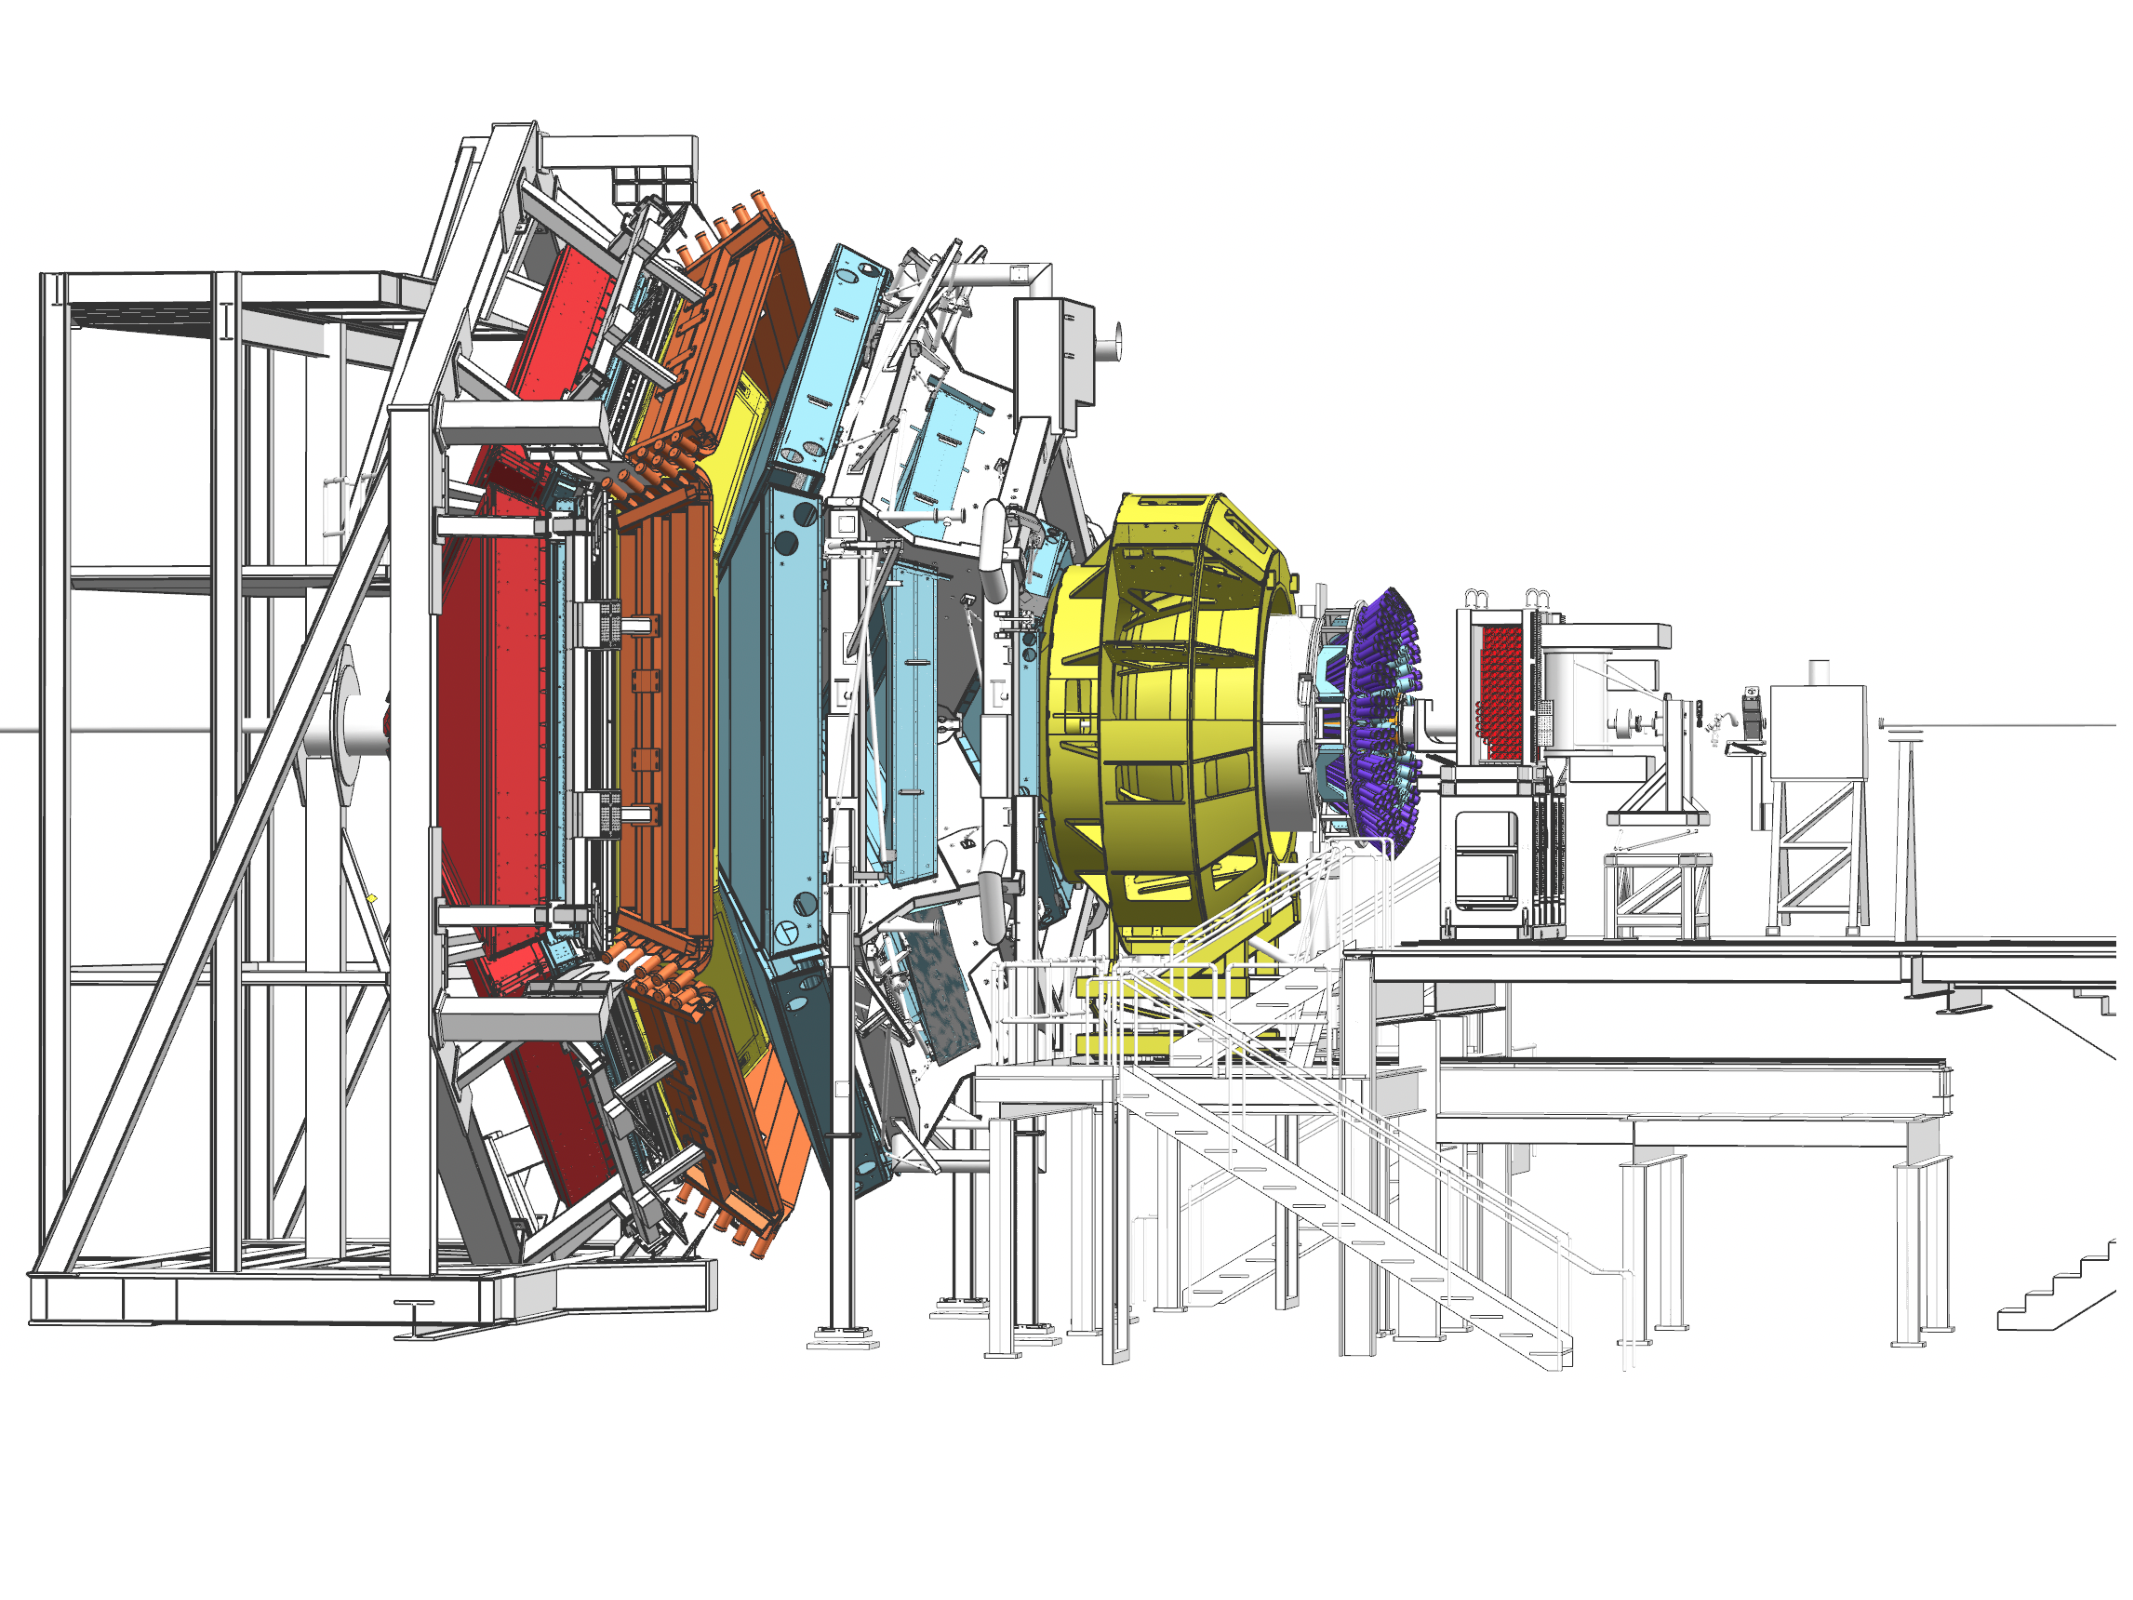
\includegraphics[width=0.48\textwidth]{BandInClas.pdf}
	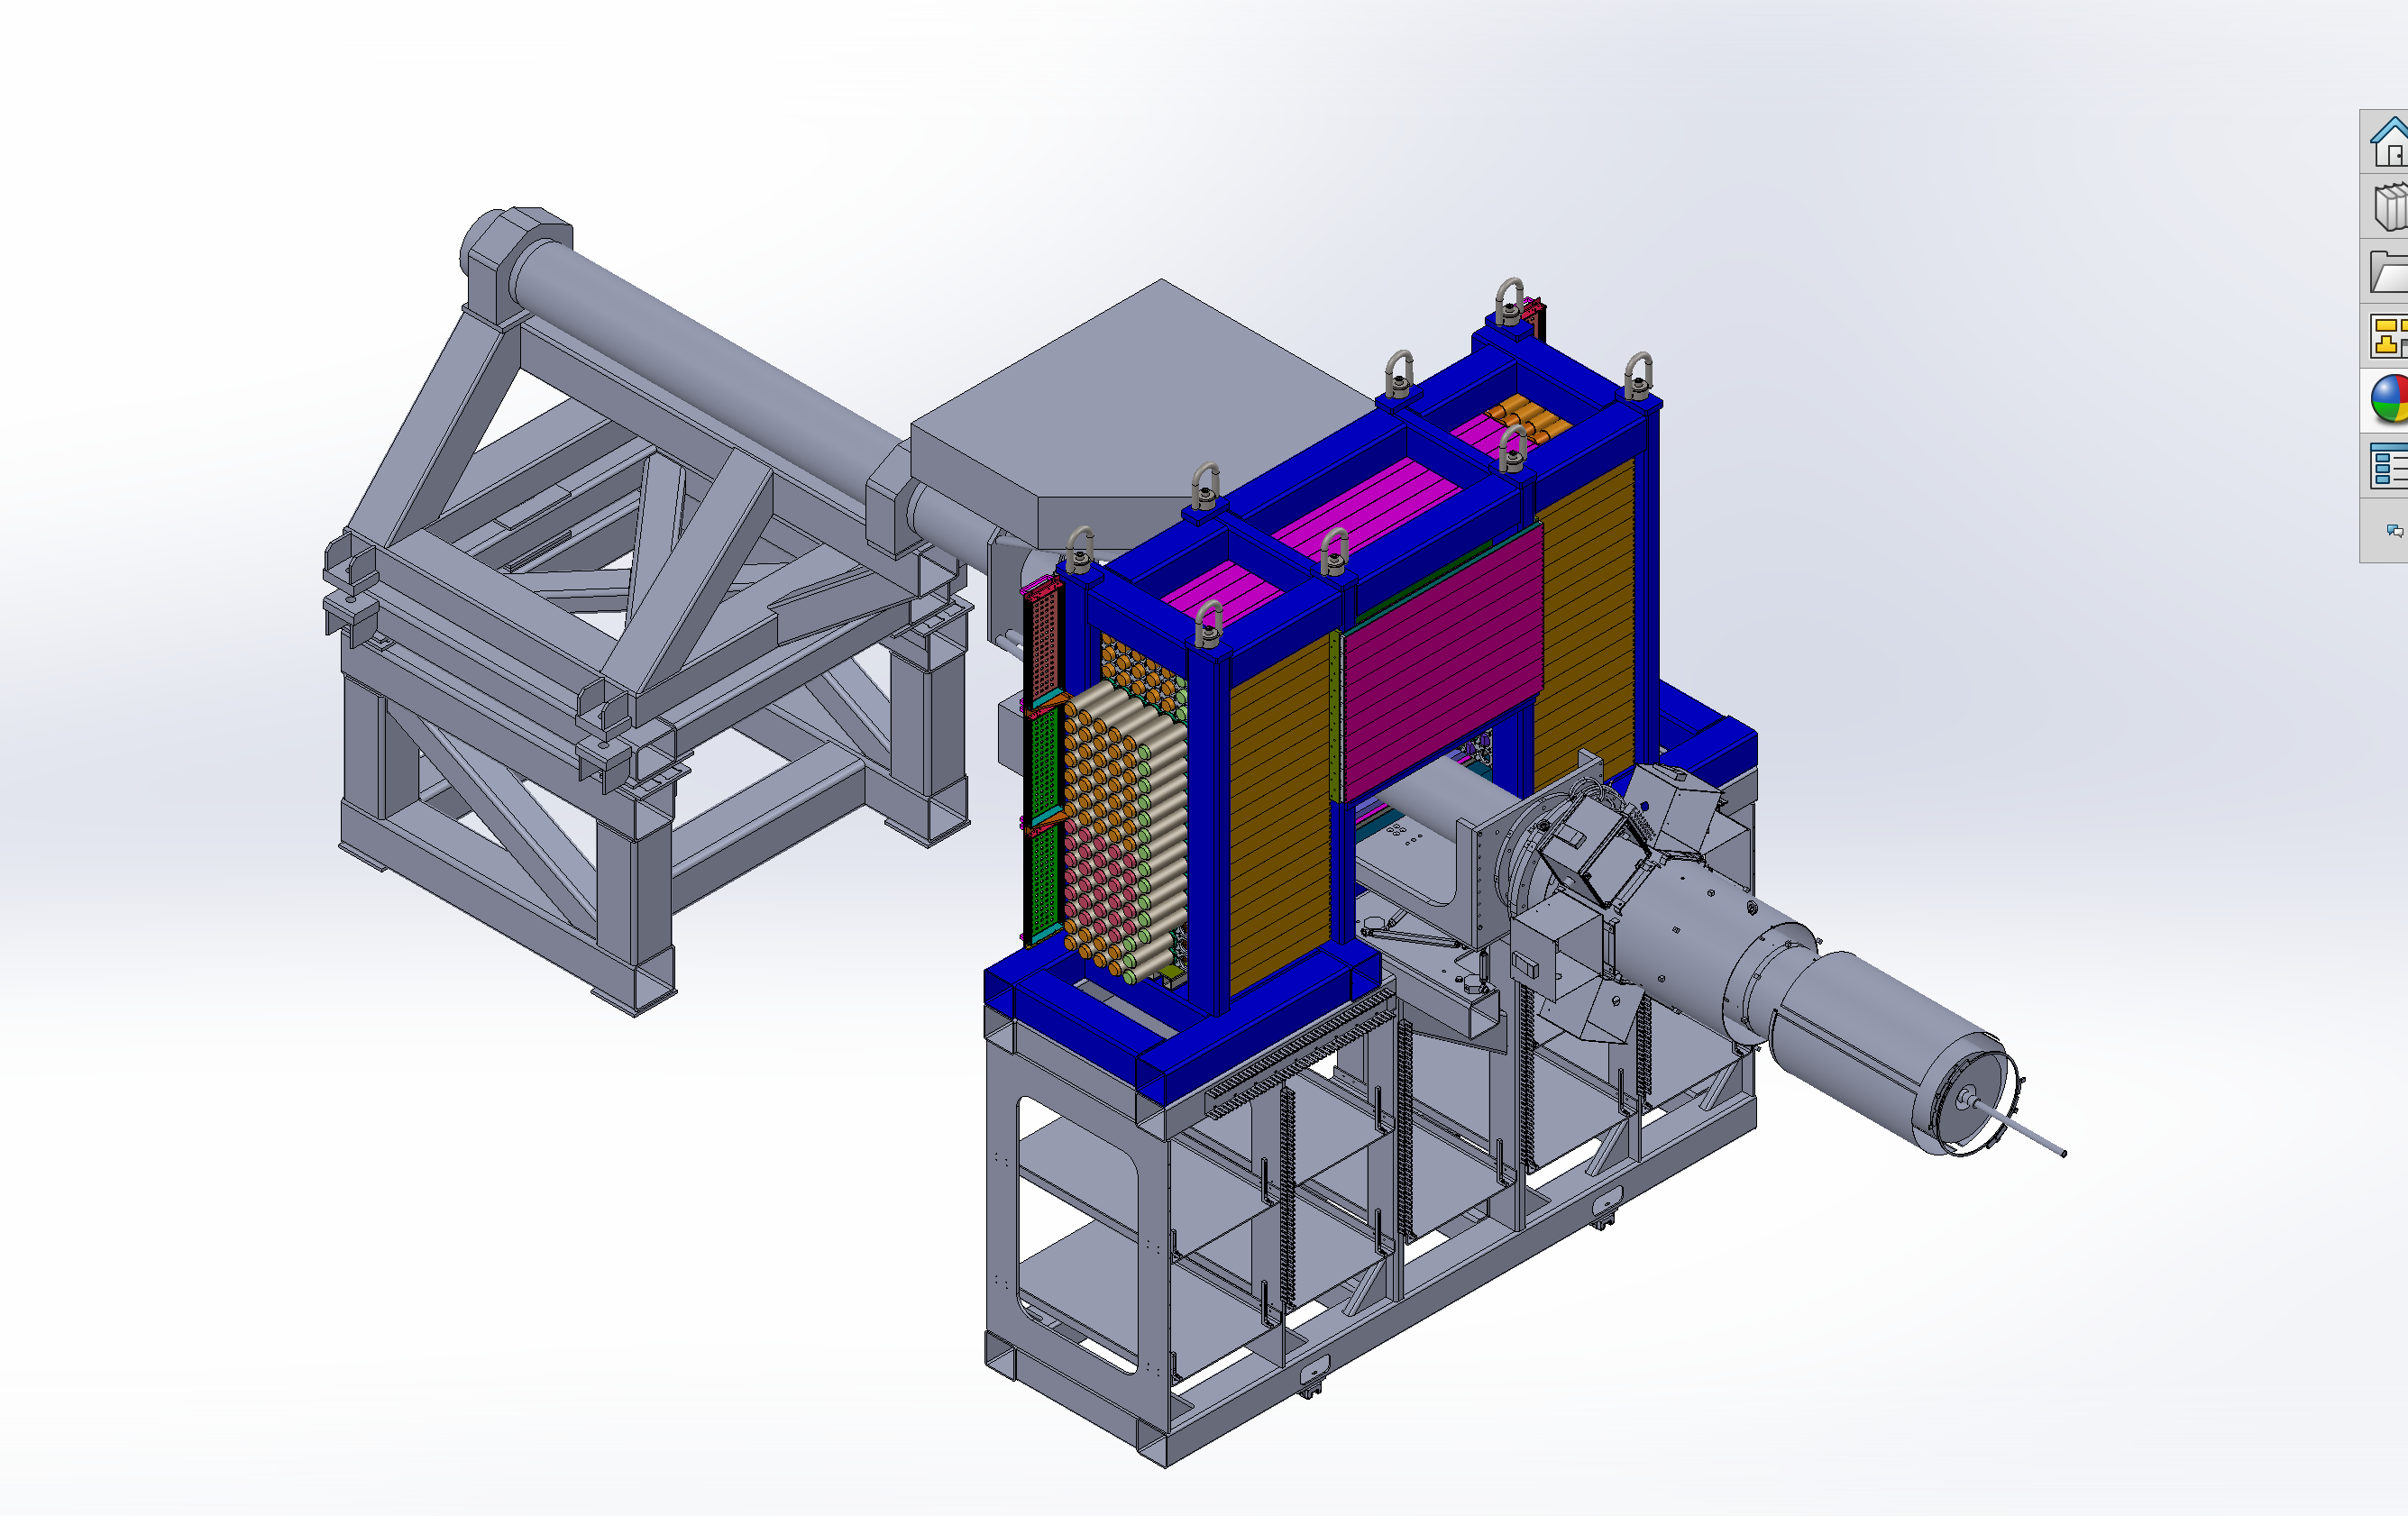
\includegraphics[width=0.48\textwidth]{BandInContext1.png}
		\caption{BAND with CLAS12}
		\label{fig:clas12}
\end{figure}


%%%%%%%%%%%%%%%%%%%%%%%%%%%%%%%%%%%%%%%%%%%%%%%%%%%%%%%%%%%%%%%%%%%%%%%%%%%%%%%%%%%%%%%%%%%%%%%%%%%

\section{Design of the backward angle neutron detector}
To achieve the physics channels of interest with neutrons in the BAND, time-of-flight (ToF) resolutions below $300$ \si{\pico\second} and XXX path length 
resolution are required for the scintillant detector {\color{red}(and neutron PID?)}. {\color{red}These design parameters... (why are these the 
design parameters)}. Neutral-particle identification is established via vetoing algorithms ({\color{red}see online supplemental materials}) aided by
a thin $1$ \si{\centi\meter} veto layer for charged-particle identification. Neutron-photon discrimination is achieved with ToF separation given the design 
timing resolutions. Furthermore, off-time random neutron contamination can be controlled with signal energy deposit. {\color{red} Any need to mention 
the raw rates that we need to handle in CLAS12?} 

\subsection{Geometry}
The geometry of the BAND was constrained by the physics of interest (i.e. backward-going neutrons) \cite{Emcsrcdeens} and the available space in the hall. To
maximize the fiducial volume inside of hall constraints, a design of rectangular scintillant bars that are layered in $z$ and $y$ was chosen; see Fig.~\ref{fig:design}.
The cross section of each scintillator bar determines our position granularity in $y,z$, and was chosen such that it yields comparable uncertainty to $x$ given the bar 
time resolutions. With a design ToF resolution below $300$ \si{\pico\second}, $7.2$ \si{\centi\meter} by $7.2$ \si{\centi\meter} scintillator bars were chosen to optimize
fiducial volume, granularity, and cost.
\begin{figure}[h]
	\centering
		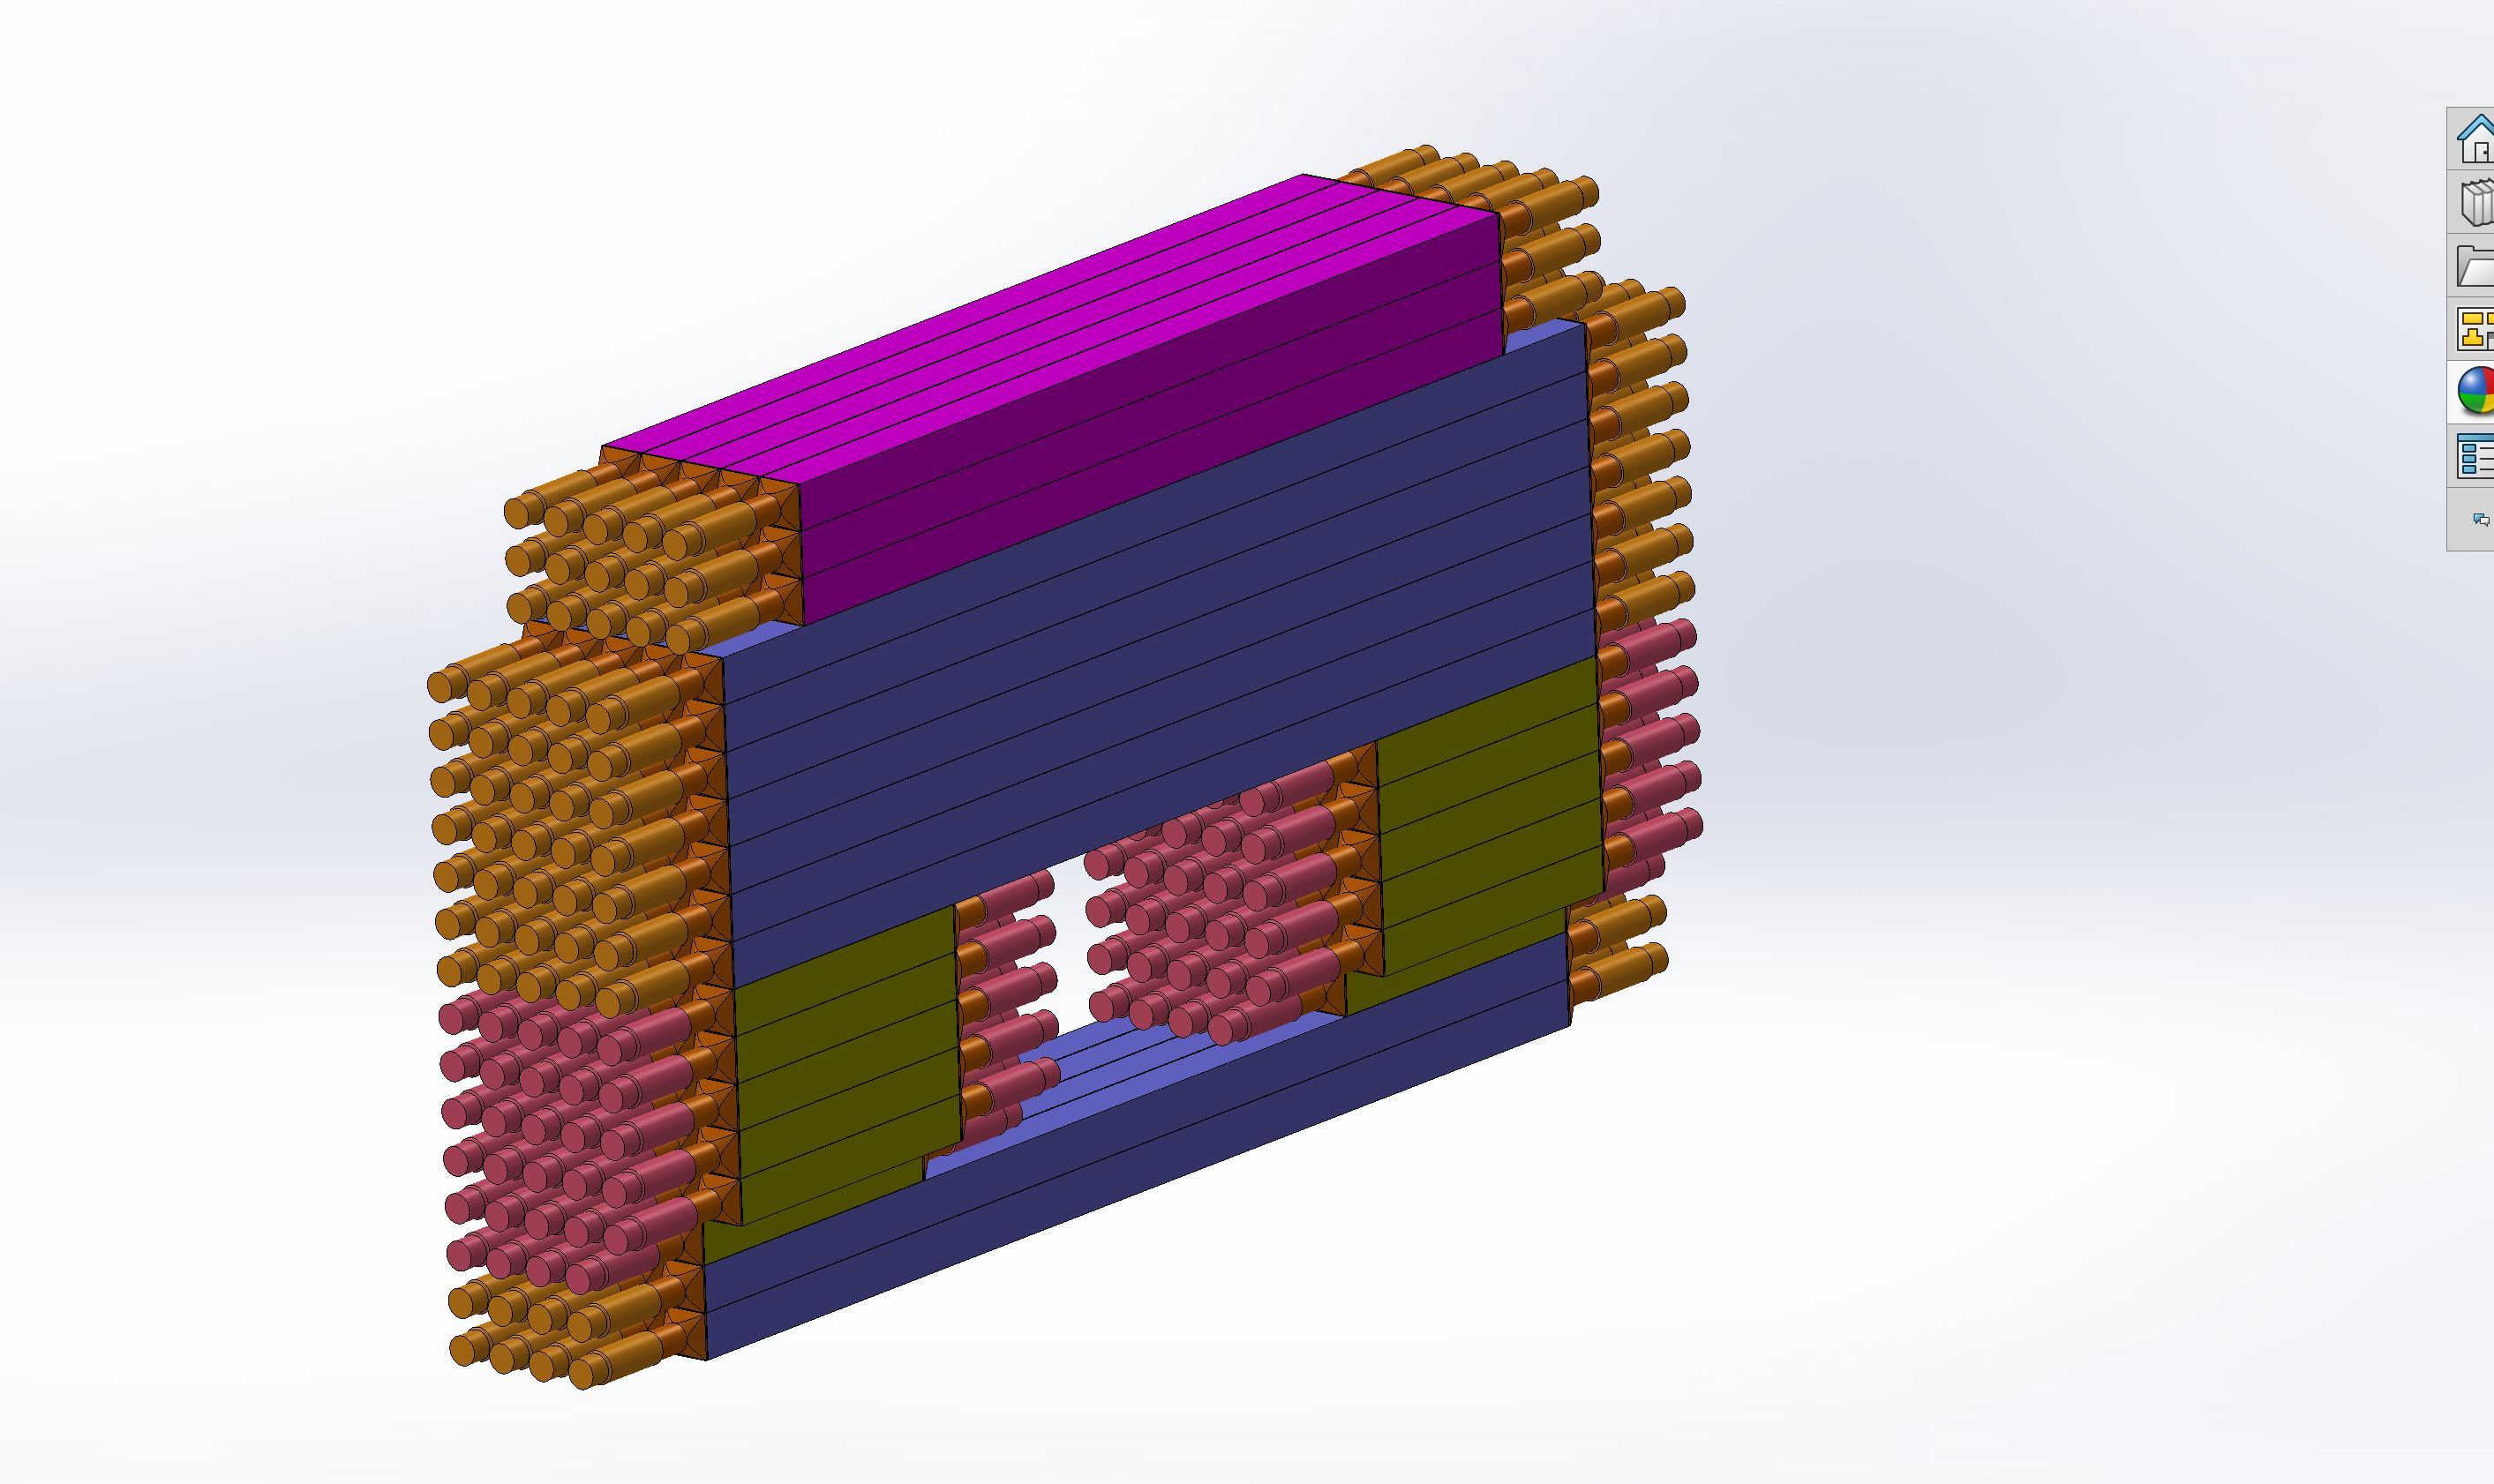
\includegraphics[width=0.48\textwidth]{Band01.png}
		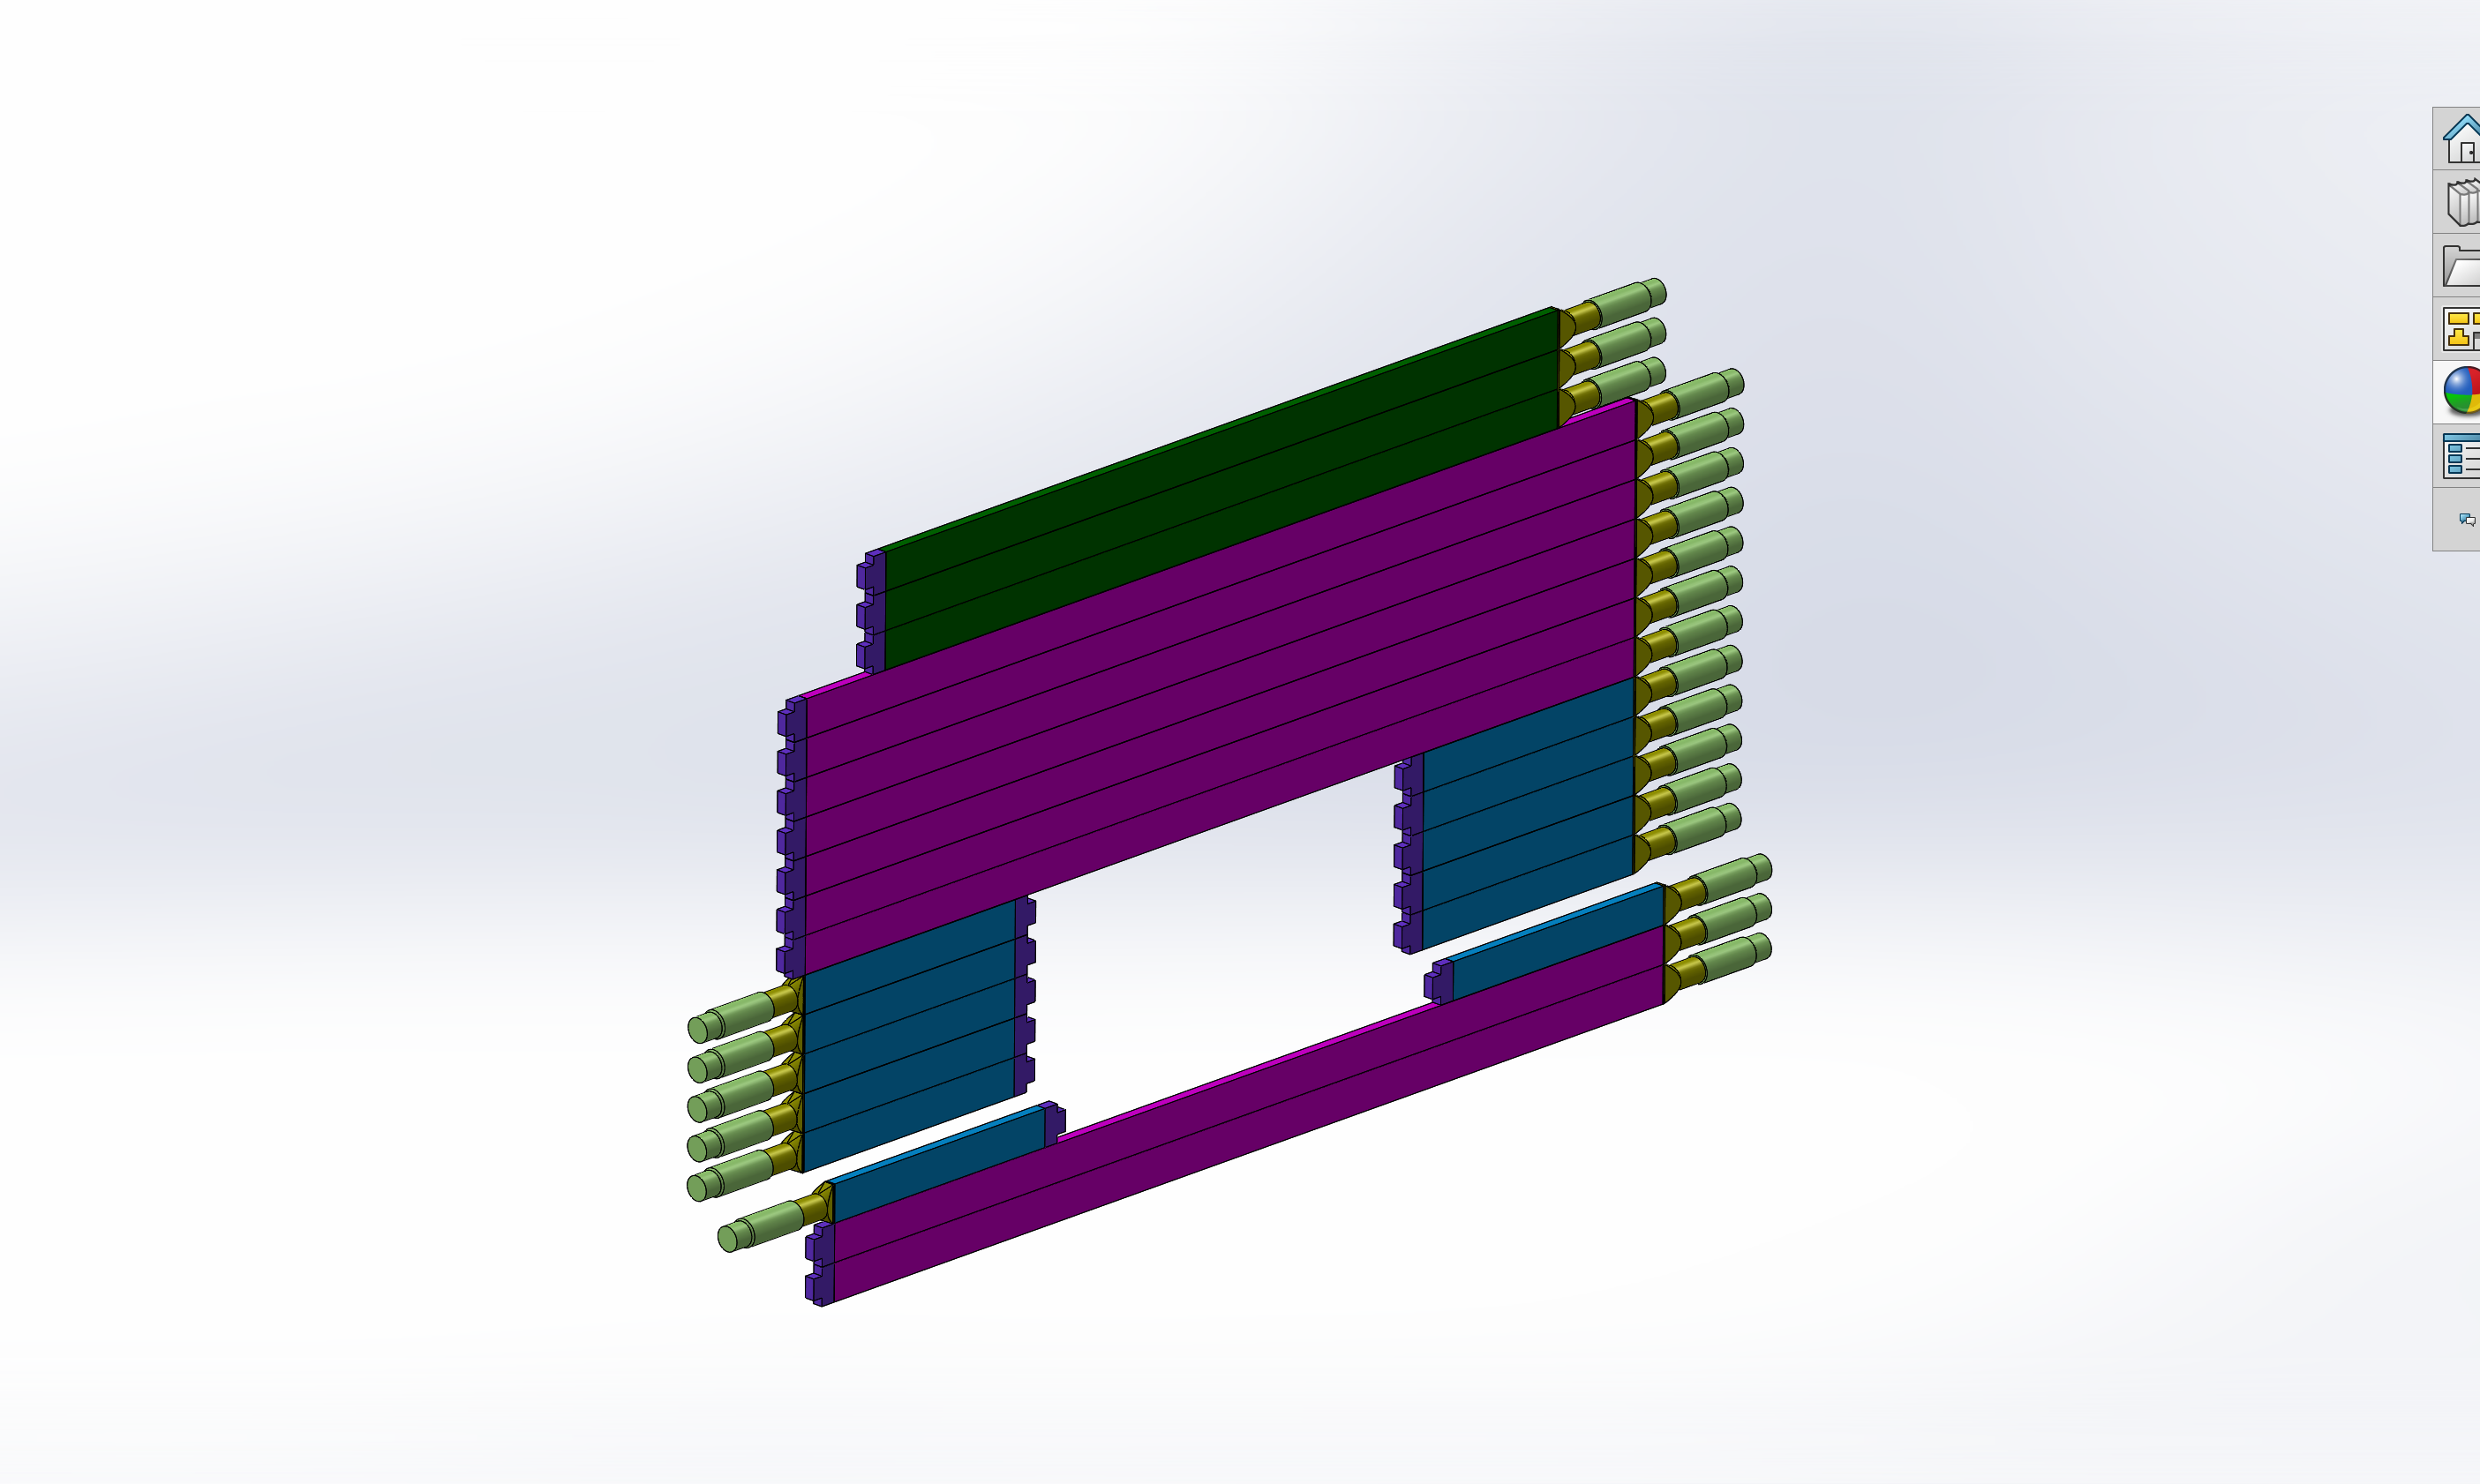
\includegraphics[width=0.48\textwidth]{BandVeto.png}
		\caption{BAND design. Need an updated nicer figure with direction of beam / coordinate system. Also have a similar 
		color scheme denoting the different sectors, so let's do a darker/ligher shade of green for the short bars so we can make 
		a table of sector, layer, ID, etc..}
		\label{fig:design}
\end{figure}

\subsection{Calibration system}
Due to the placement of the BAND, in CEBAF 12 \si{\giga\electronvolt} with the CLAS12 magnetic fields [{\color{red}CITE}], there is a lack of exclusive processes 
that can be used for monitoring performance stability. A laser system [{\color{red}CITE}] was implemented to validate performance during data-taking. This system also 
provided a method to quickly perform calibrations (discussed below).

\subsection{Components}
The timing resolution of the scintillator bars is impacted by many factors, and each component was optimized considering the design constraint and cost. Tests were 
performed varying the scintillant, reflective wrapping, photo-multipler tube (PMT), and optical-coupling-method of the scintillators to light-guides to PMTs; see 
Table~\ref{tab:tests} and Fig.~\ref{fig:test_stand}. 

To extract the time resolution of a PMT, we make use of a coincidence signal between a ``test" scintillator bar and a ``reference" scintillator bar. Each bar has 2 PMTs 
coupled to the ends; the test bar has the PMTs which we wish to measure the time resolution. Both bars are wrapped in an optical reflector, and made light-tight 
via use of tape, coverings, and a black-box. The reference bar parameters are never changed during any measurement. 

A $^{60}$Co source is used as a coincidence signal between the two bars. $^{60}$Co undergoes $\beta^-$ decay to an excited state $^{60}$Ni, which then undergoes 
two $\gamma$ decays down to a $0^+$ ground state (1.17, 1.33 MeV respectively). The two $\gamma$-rays being angularly correlated have a preferred back-to-back 
emission of 180$\degree$. The $^{60}$Co source is collimated by two lead bricks to deposit the $\gamma$-rays at specific locations along the bars, allowing for the 
study of PMT time resolution as a function of distance from the PMT (or, due to attenuation along the bar, effective-energy observed by the PMT).

\begin{table}[t!]
	\caption{Tested configurations. Resolution given $2$ \si{\mega\electronvolt} energy deposit in middle of bar.}
	\begin{tabular}{  m{5em} | m{4em} | m{5em} | m{4em} | m{3em} |  m{5.7em} | m{4em} }
		\hline
			Scintillator & Reflector & PMT & Optical-coupling & Length (cm) & Cross section (\si{\centi\meter} x \si{\centi\meter}) & $\sigma$ (\si{\pico\second})\\
		\hline
		\hline
			EJ-200 & Al foil & ET-9214 & Grease & 200 & 7 x 7 & 270			\\
		
			EJ-200 & Al foil & R7724-10 & Grease & 200 & 7 x 7 & 240		\\
			EJ-200 & Al foil & R13435 & Grease & 200 & 7 x 7 & 300 			\\
		
			EJ-200 & Al foil & R13089 & Grease & 250 & 5 x 5  & 220			\\
			EJ-200 & Al foil & R7724-100 & Grease & 250 & 5 x 5 & 200 		\\
			
			BC-408 & XXX & ET-9214 & RTV 615 &50 & 7 x 7 & 150				\\
			BC-408 & XXX & R7724-10 & RTV 615 & 200 & 7 x 7 & 150			\\
		\hline
	\end{tabular}
	\label{tab:tests}
\end{table}

\begin{figure}[h!]
	\centering
	\begin{minipage}{0.48\textwidth}
		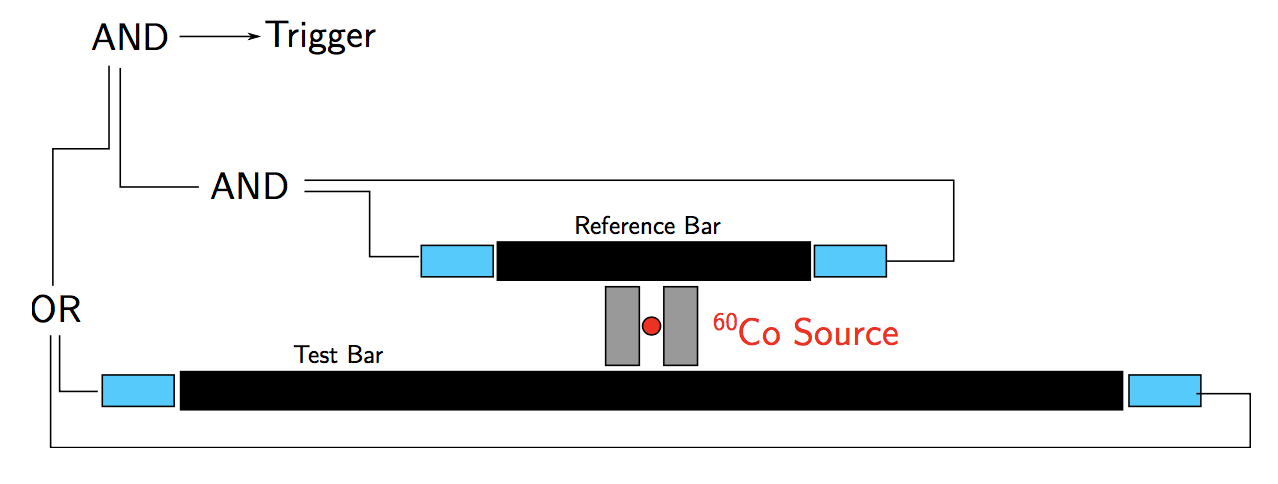
\includegraphics[width=\textwidth]{phys_setup.png} \\
		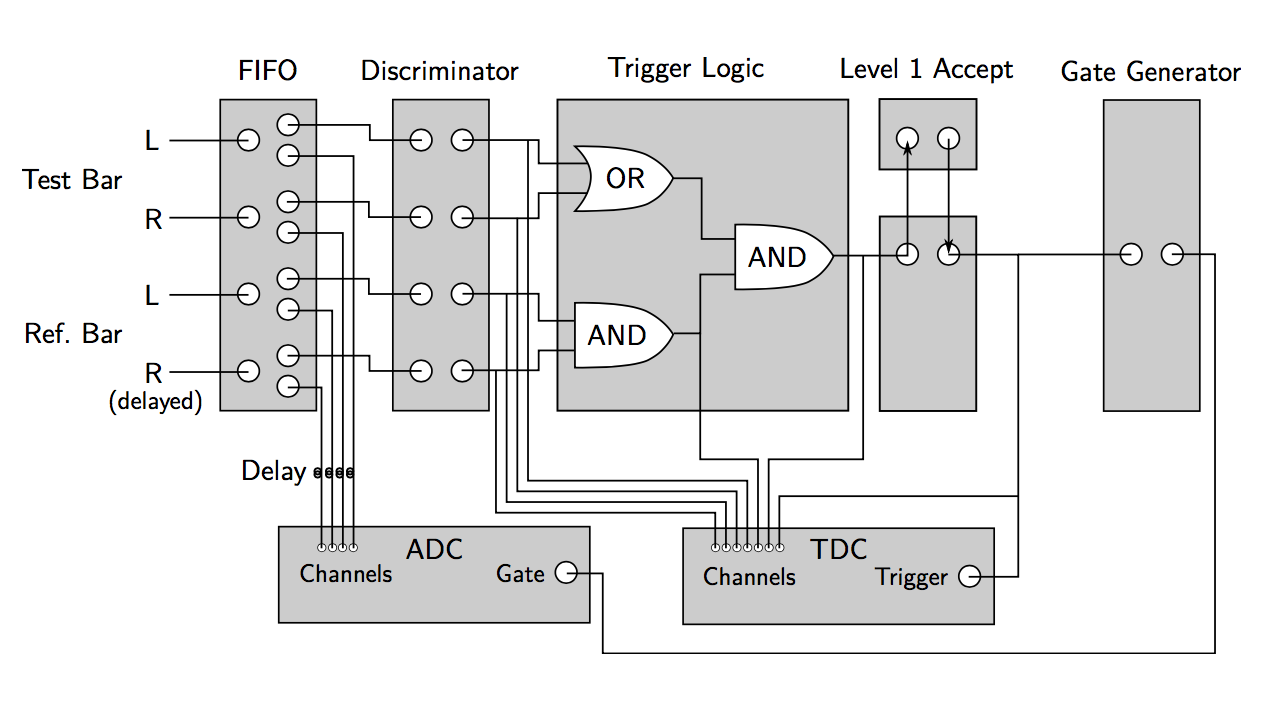
\includegraphics[width=\textwidth]{electr_setup.png}
	\end{minipage}
	\begin{minipage}{0.48\textwidth}
		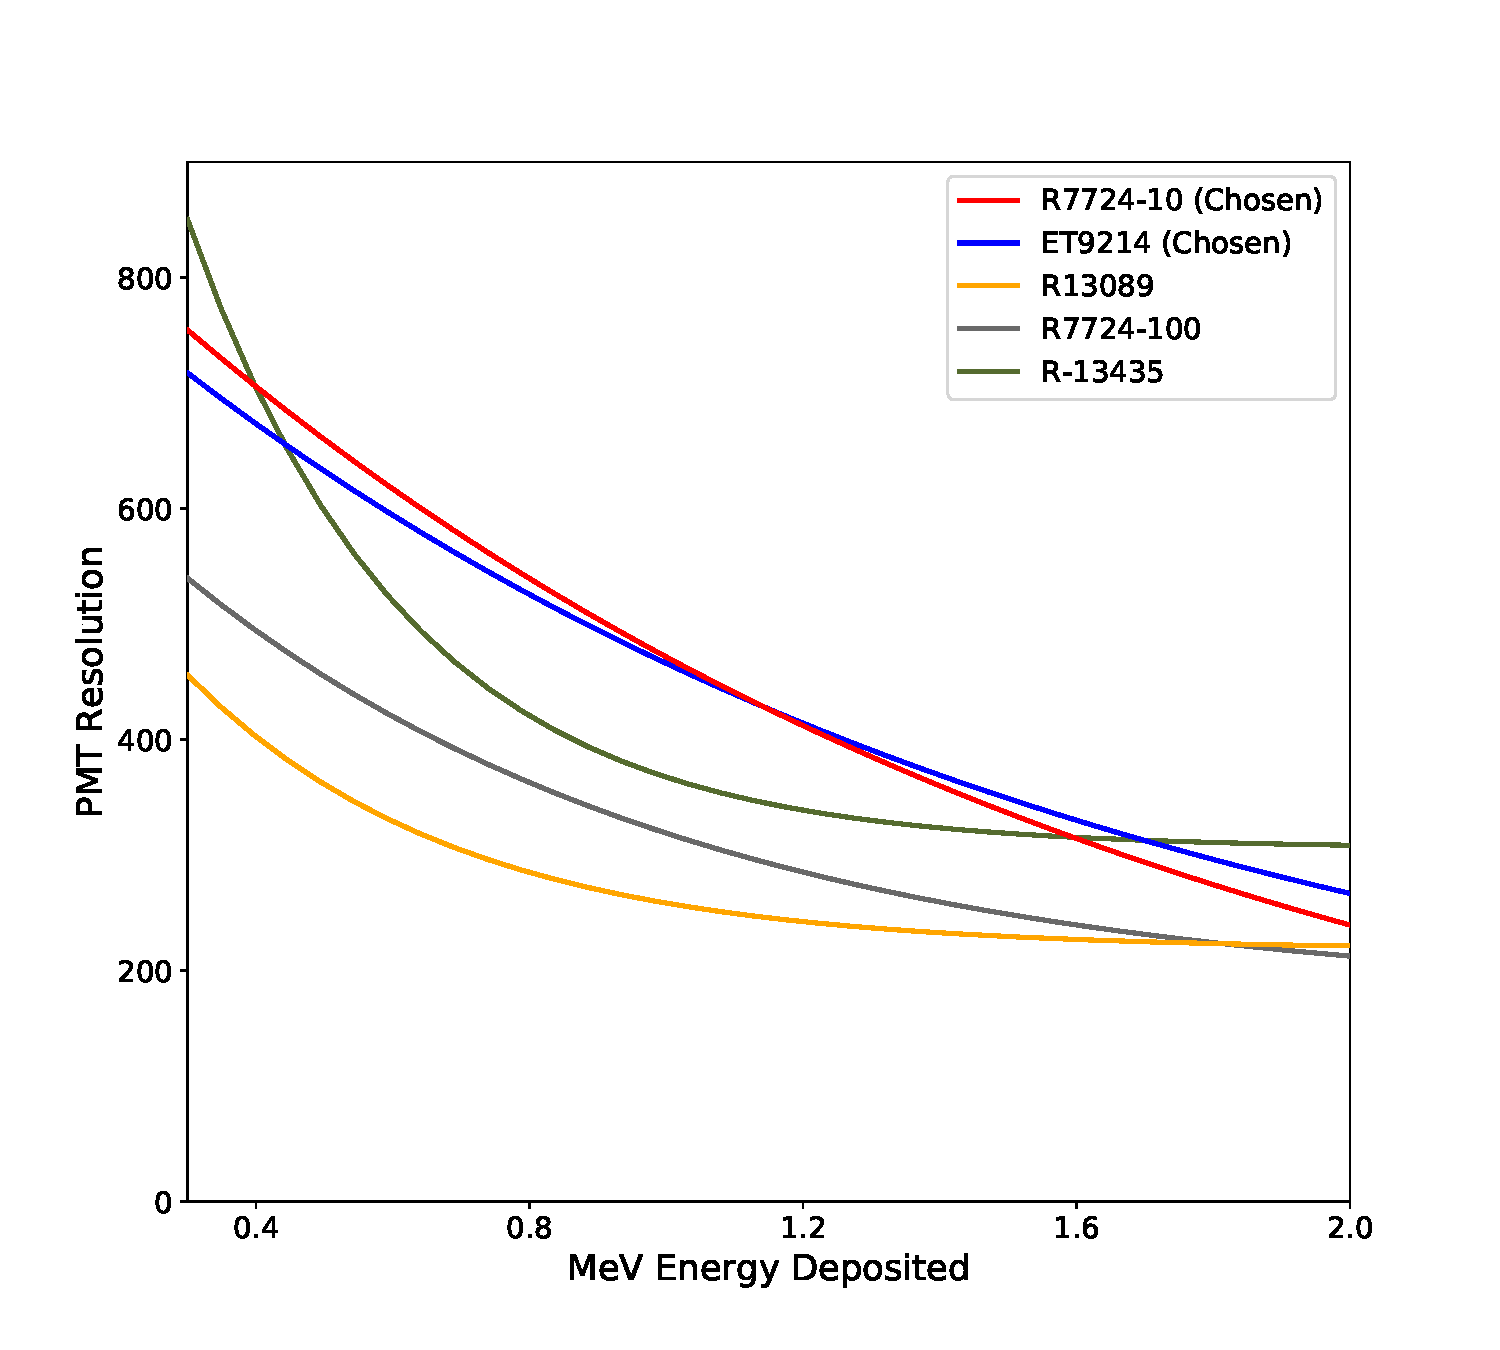
\includegraphics[width=\textwidth]{test-stand/test-resolutions.pdf}
	\end{minipage}
	\caption{Test stand setup and results}
	\label{fig:test_stand}

\end{figure}

\subsection{Magnetic shielding}
{\color{red}Another consideration was magnetic shielding. Explain.}

\subsection{Lead shielding}
{\color{red}Another consideration was lead shielding. Explain.}

%%%%%%%%%%%%%%%%%%%%%%%%%%%%%%%%%%%%%%%%%%%%%%%%%%%%%%%%%%%%%%%%%%%%%%%%%%%%%%%%%%%%%%%%%%%%%%%%%%%

\section{Description}
All the parts, models, electronics, etc..

\section{Performance}
All the calibrations, and results

\clearpage



%%%%%%%%%%%%%%%%%%%%%%%%%%%%%%%%%%%%%%%%%%%%%%%%%%%%%%%%%%%%%%%%%%%%%%%%%%%%%%%%%%%%%%%%%%%%%%%%%%%
%%%%%%%%%%%%%%%%%%%%%%%%%%%%%%%%%%%%%%%%%%%%%%%%%%%%%%%%%%%%%%%%%%%%%%%%%%%%%%%%%%%%%%%%%%%%%%%%%%%
%%%%%%%%%%%%%%%%%%%%%%%%%%%%%%%%%%%%%%%%%%%%%%%%%%%%%%%%%%%%%%%%%%%%%%%%%%%%%%%%%%%%%%%%%%%%%%%%%%%
%%%%%%%%%%%%%%%%%%%%%%%%%%%%%%%%%%%%%%%%%%%%%%%%%%%%%%%%%%%%%%%%%%%%%%%%%%%%%%%%%%%%%%%%%%%%%%%%%%%
%%%%%%%%%%%%%%%%%%%%%%%%%%%%%%%%%%%%%%%%%%%%%%%%%%%%%%%%%%%%%%%%%%%%%%%%%%%%%%%%%%%%%%%%%%%%%%%%%%%
%%%%%%%%%%%%%%%%%%%%%%%%%%%%%%%%%%%%%%%%%%%%%%%%%%%%%%%%%%%%%%%%%%%%%%%%%%%%%%%%%%%%%%%%%%%%%%%%%%%
%%%%%%%%%%%%%%%%%%%%%%%%%%%%%%%%%%%%%%%%%%%%%%%%%%%%%%%%%%%%%%%%%%%%%%%%%%%%%%%%%%%%%%%%%%%%%%%%%%%
%%%%%%%%%%%%%%%%%%%%%%%%%%%%%%%%%%%%%%%%%%%%%%%%%%%%%%%%%%%%%%%%%%%%%%%%%%%%%%%%%%%%%%%%%%%%%%%%%%%
%%%%%%%%%%%%%%%%%%%%%%%%%%%%%%%%%%%%%%%%%%%%%%%%%%%%%%%%%%%%%%%%%%%%%%%%%%%%%%%%%%%%%%%%%%%%%%%%%%%
%%%%%%%%%%%%%%%%%%%%%%%%%%%%%%%%%%%%%%%%%%%%%%%%%%%%%%%%%%%%%%%%%%%%%%%%%%%%%%%%%%%%%%%%%%%%%%%%%%%
%%%%%%%%%%%%%%%%%%%%%%%%%%%%%%%%%%%%%%%%%%%%%%%%%%%%%%%%%%%%%%%%%%%%%%%%%%%%%%%%%%%%%%%%%%%%%%%%%%%

\iffalse

\begin{itemize}
\item geometry
\begin{figure}[thb]
\centering
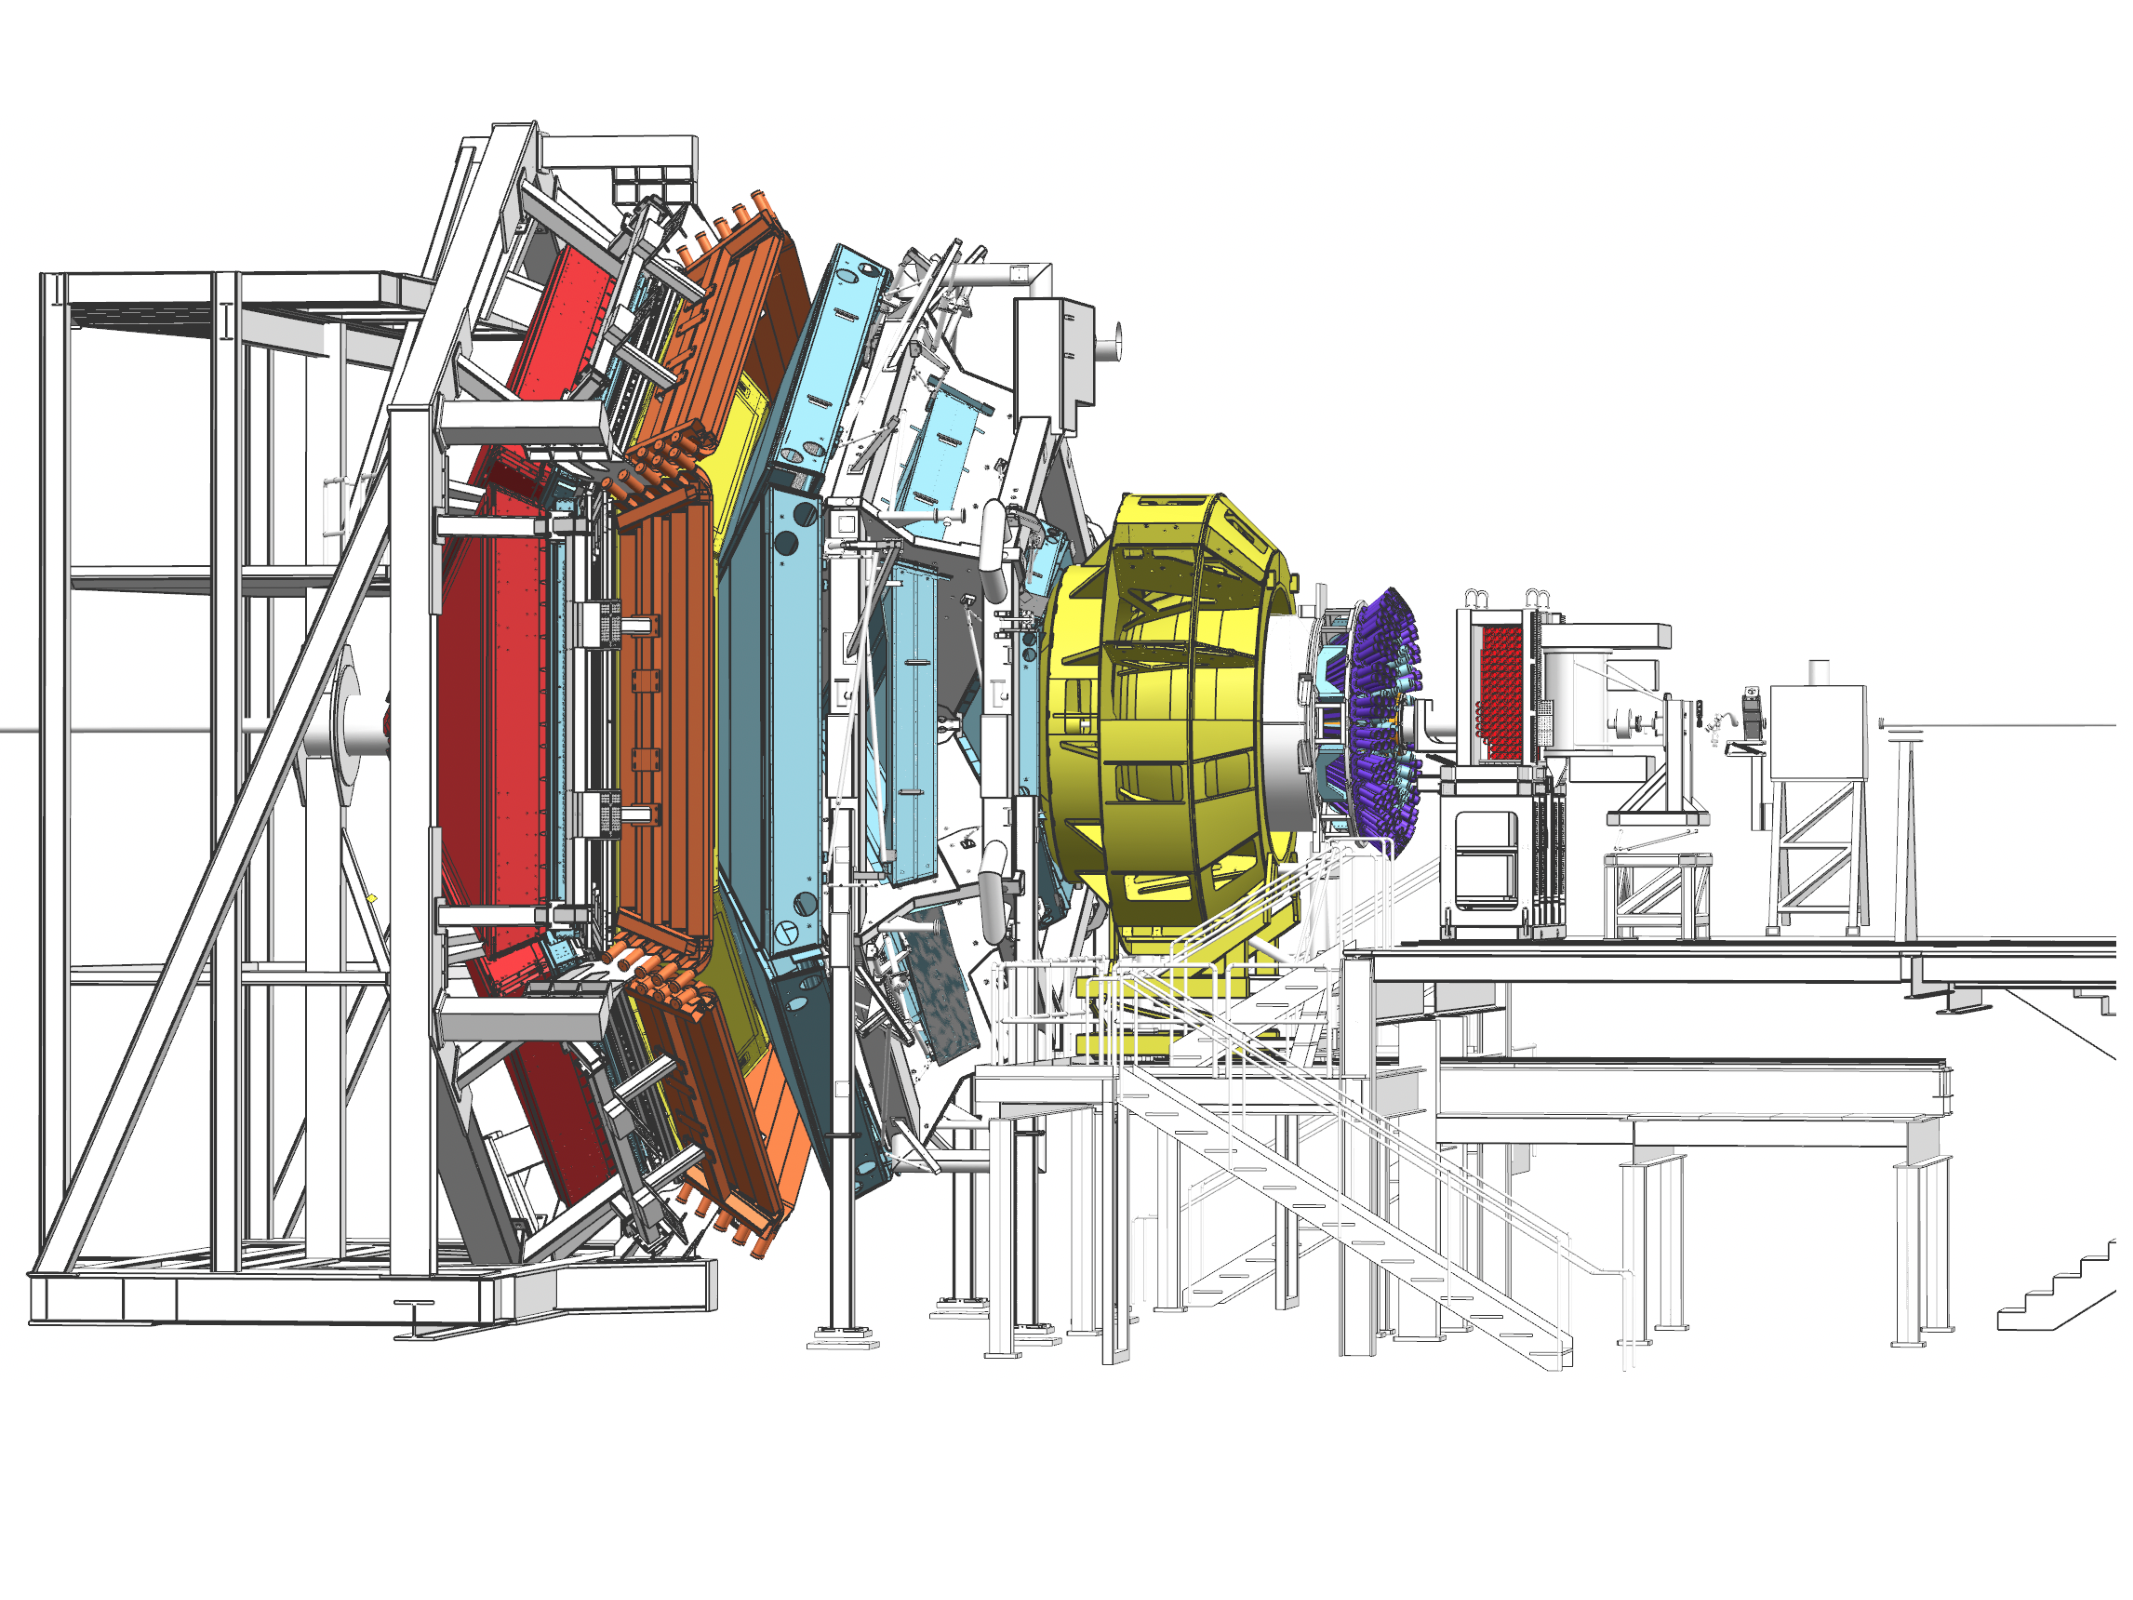
\includegraphics[width=0.96\textwidth]{BandInClas.pdf}
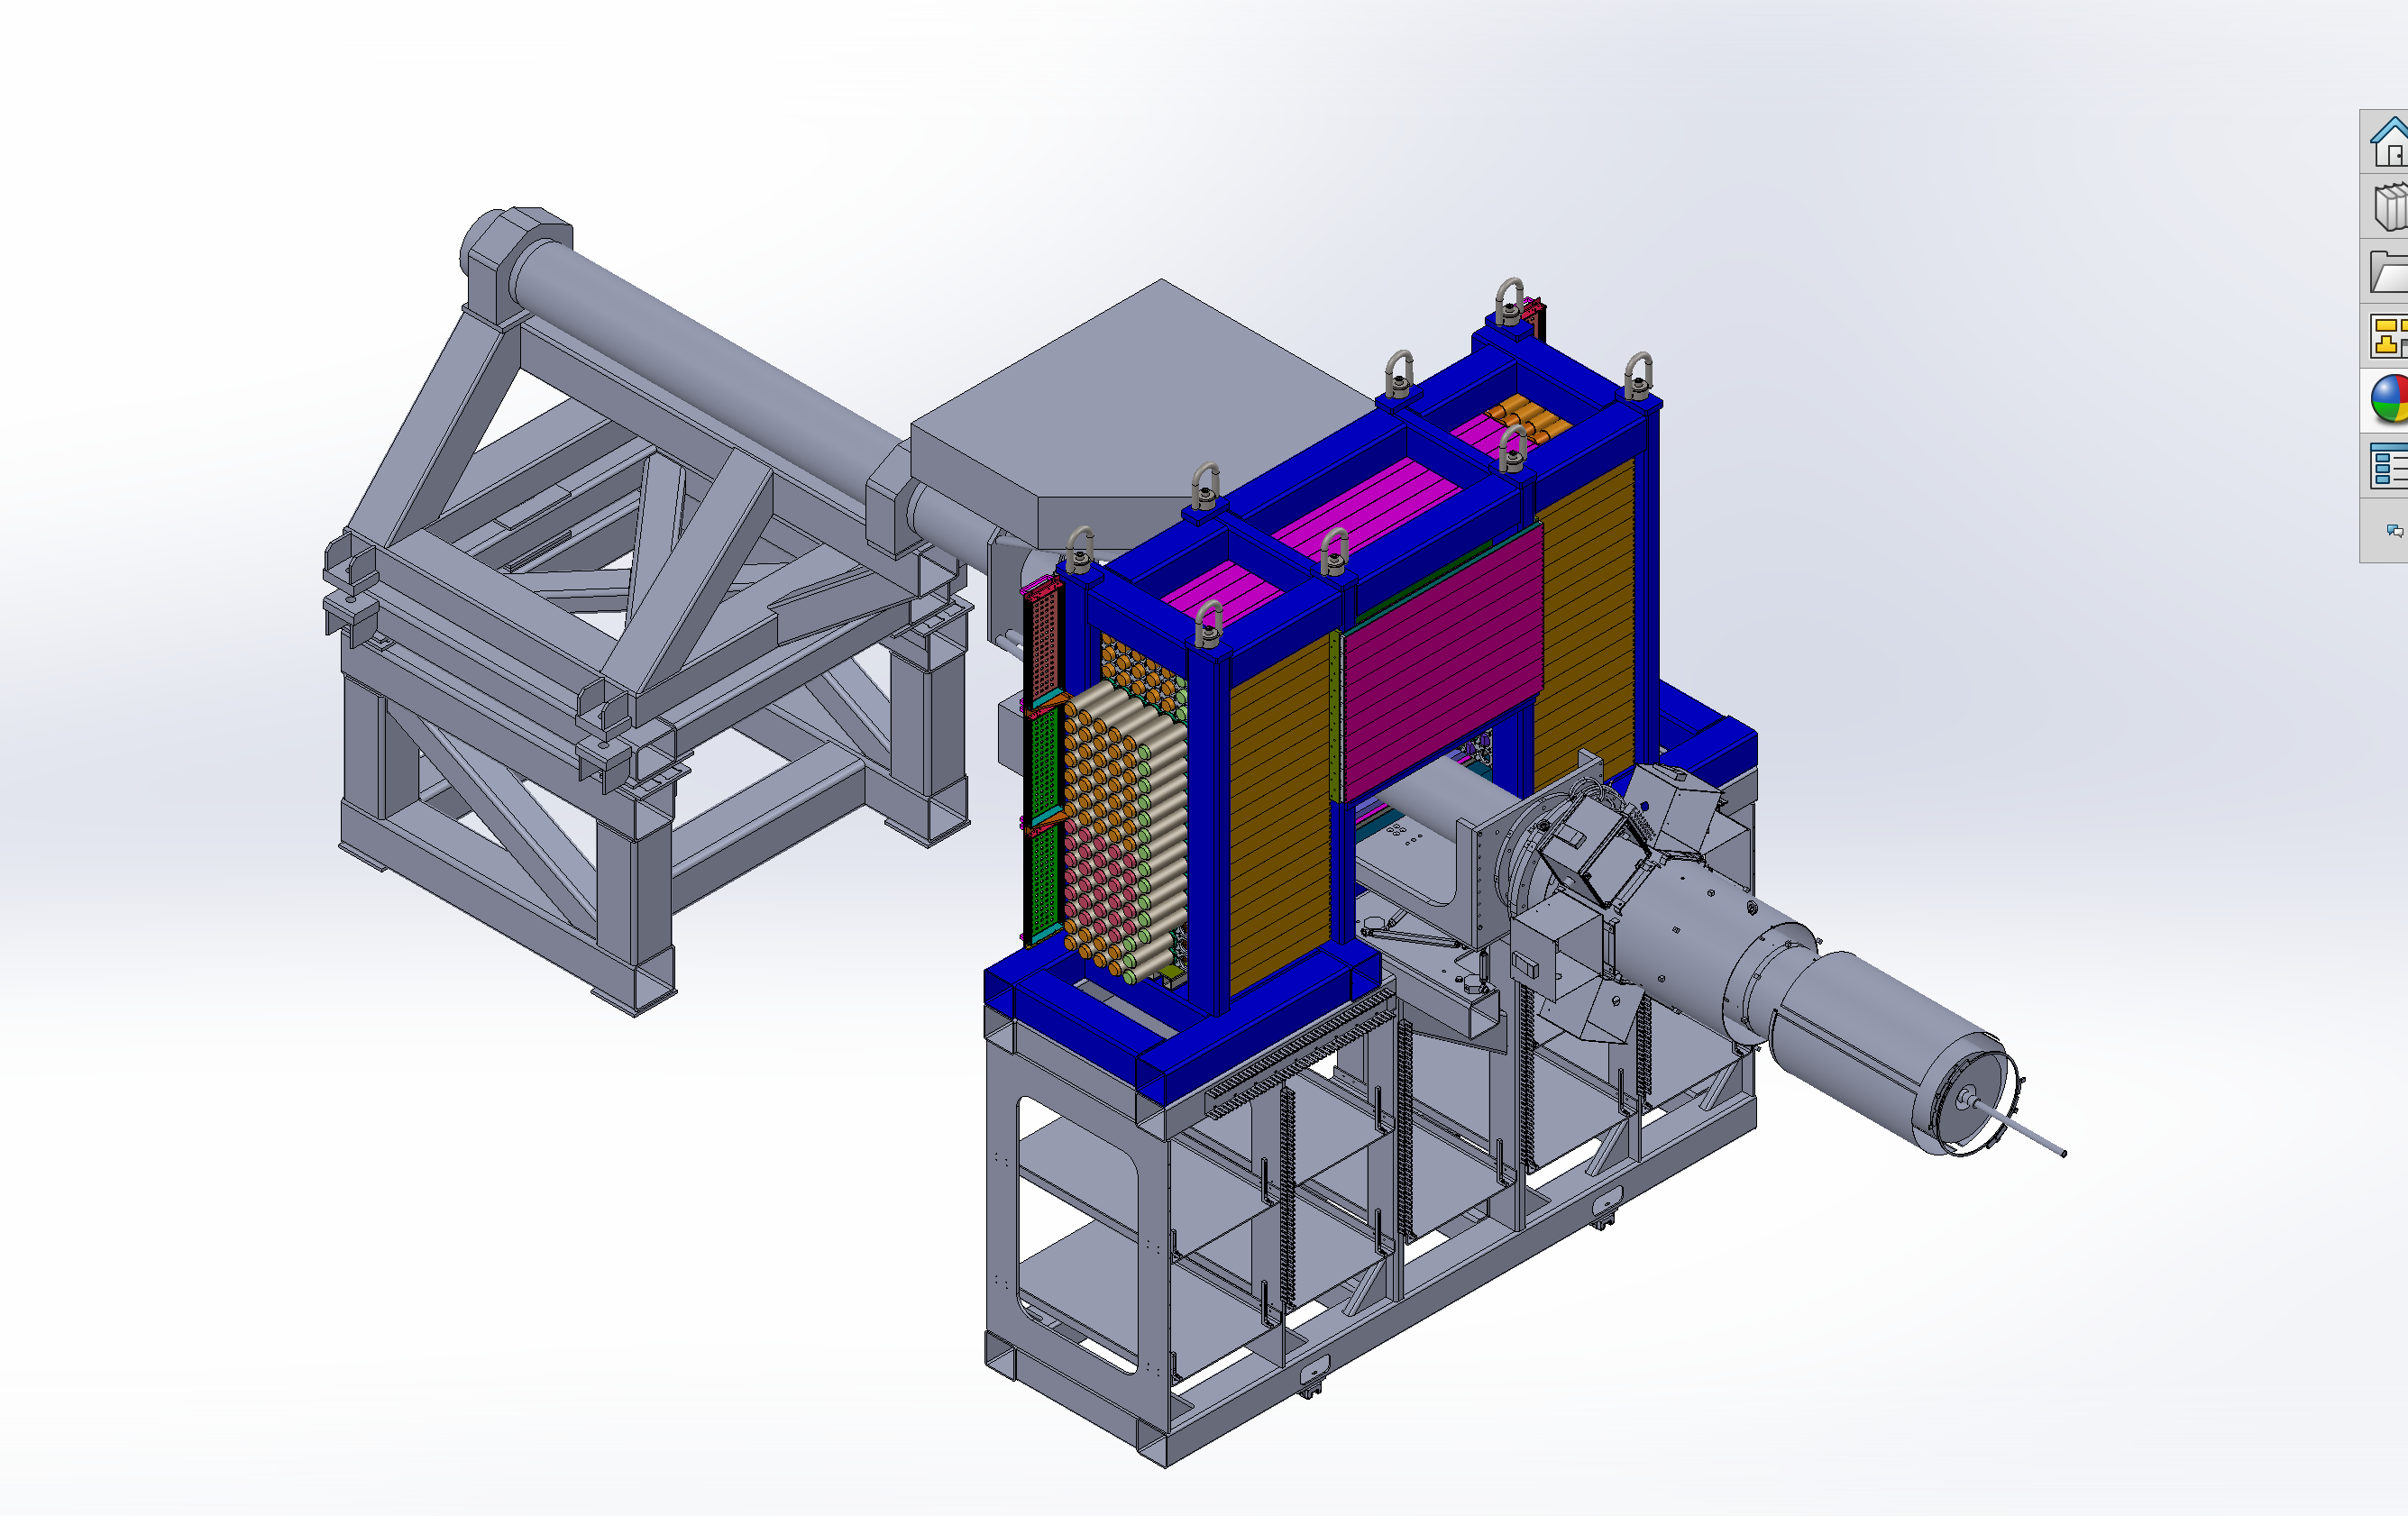
\includegraphics[width=0.48\textwidth]{BandInContext1.png}
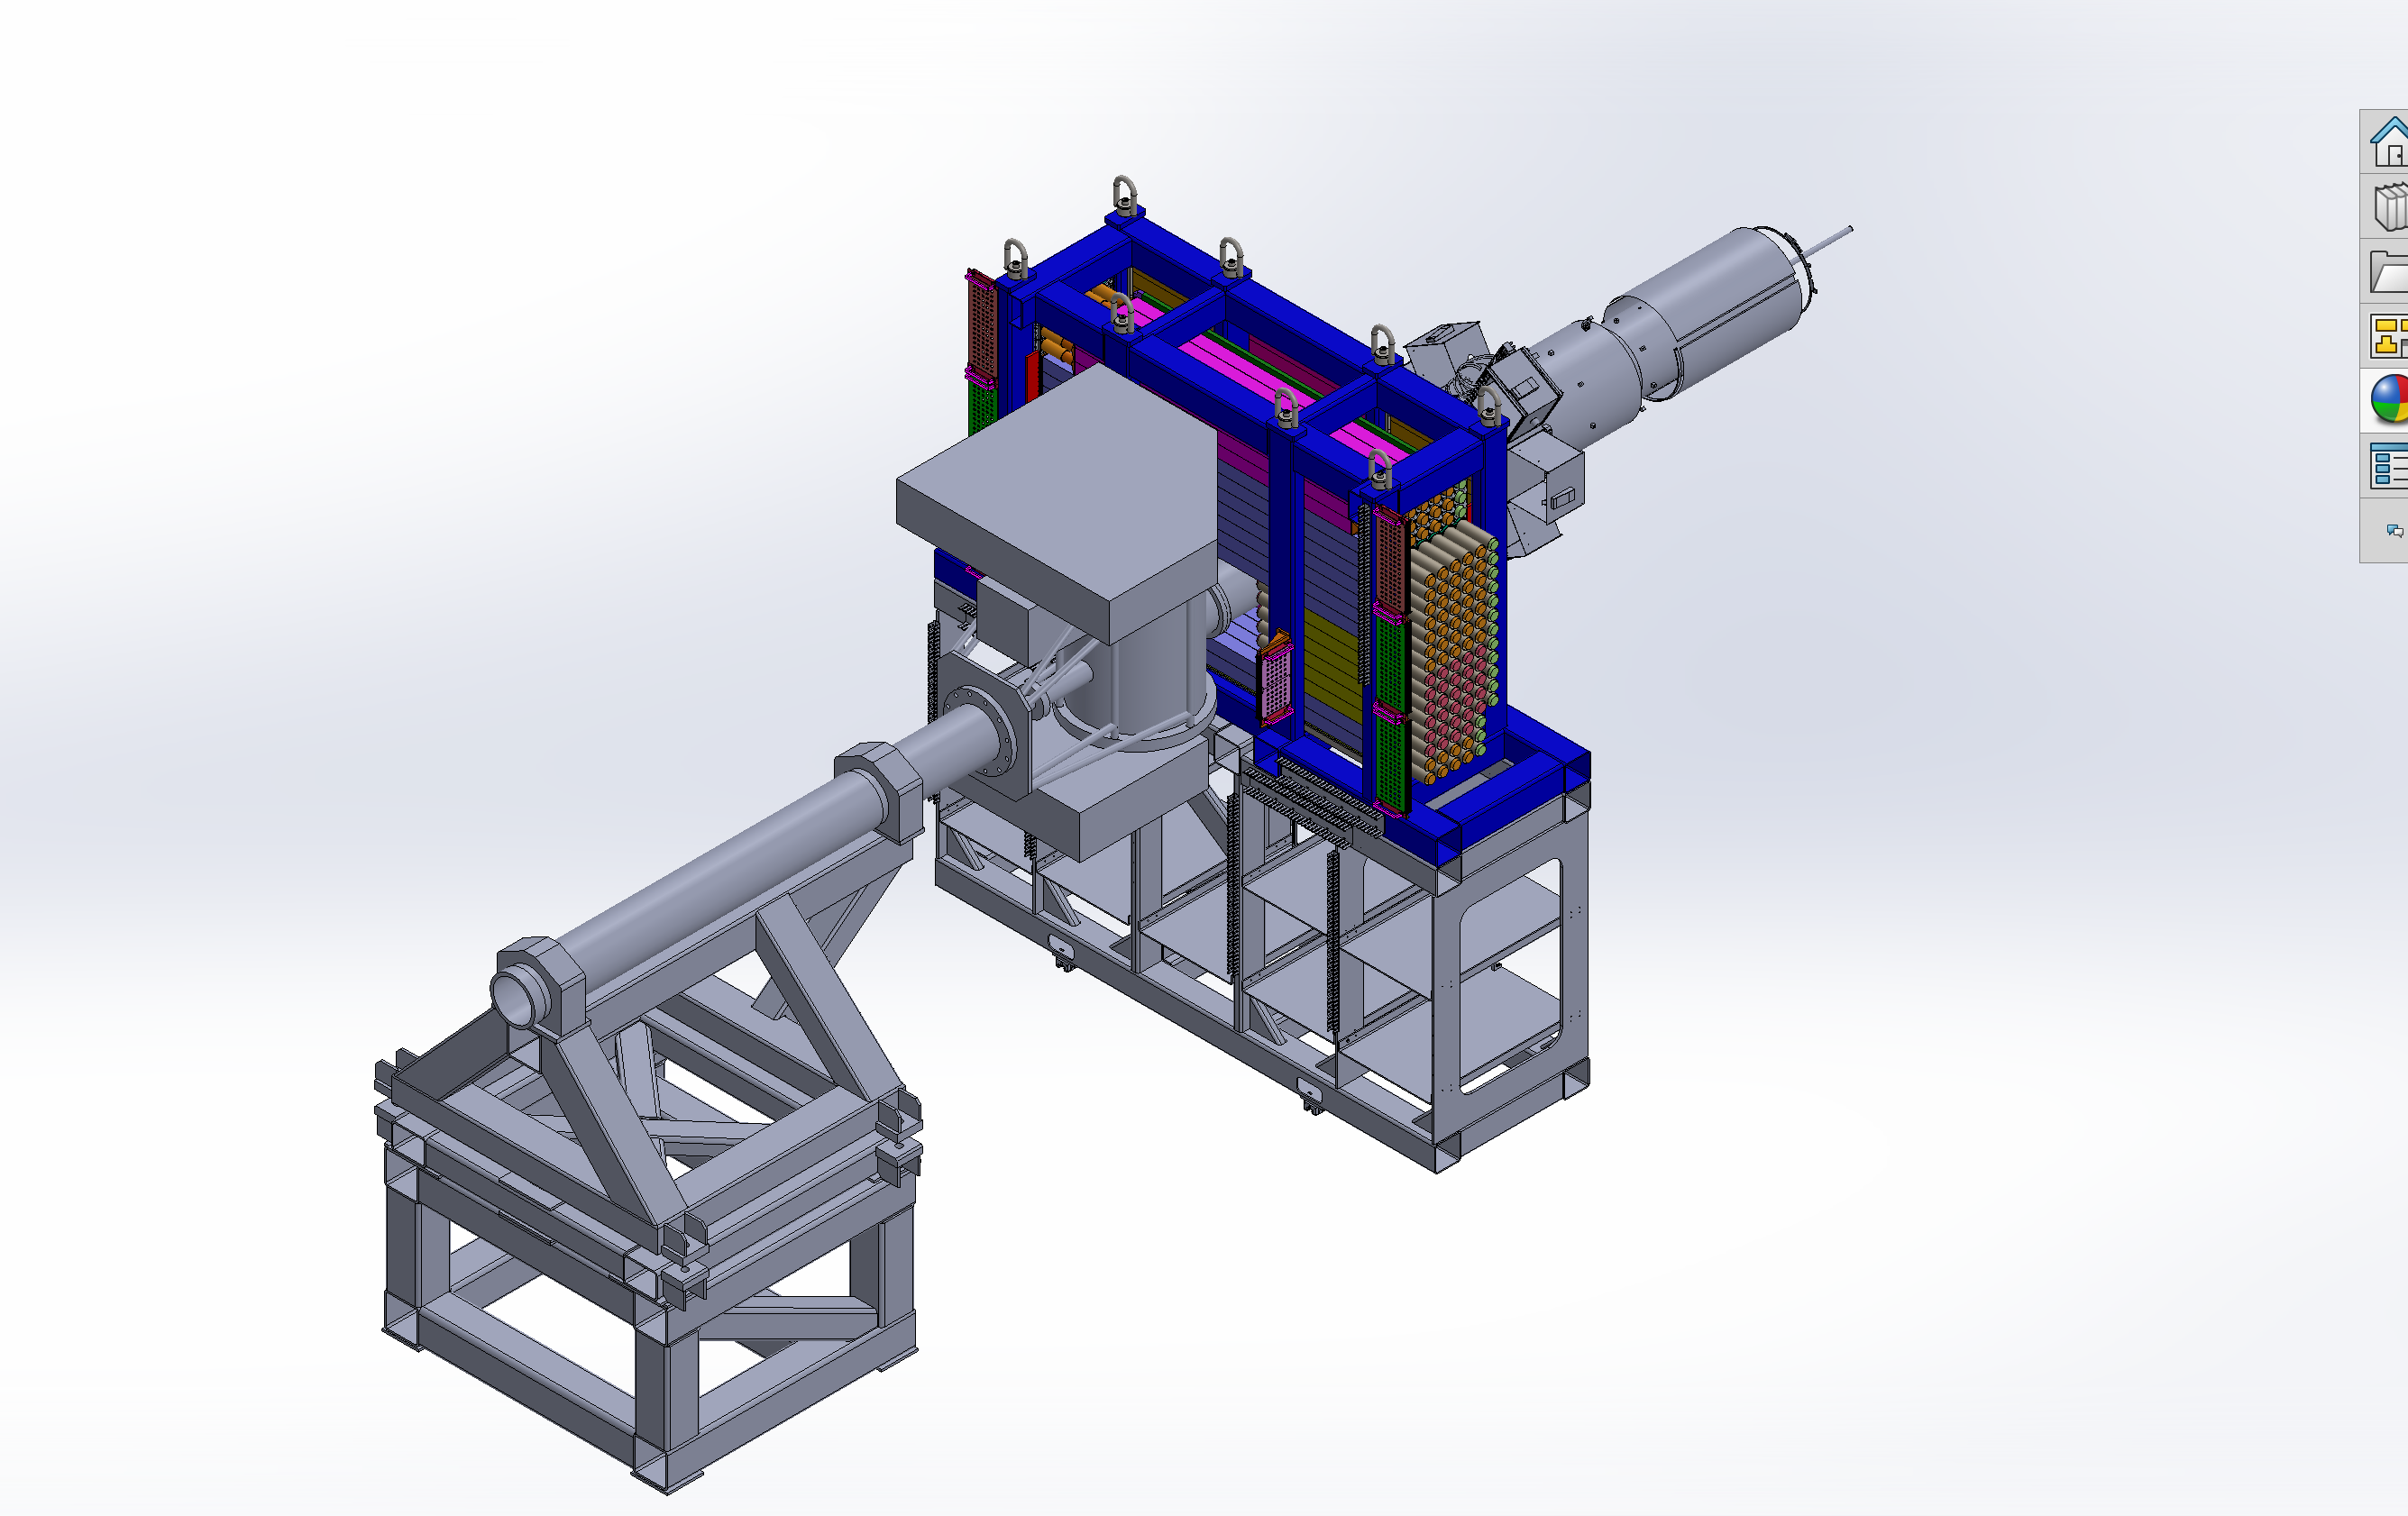
\includegraphics[width=0.48\textwidth]{BandInContext2.png}
 \caption{TODO: better picture, I don't like the options on the CAD drawing. The BAND detector is shown with its surroundings: CLAS12 target, beam line and Silicon Vertex Tracker cart. (Left) Beam is coming from top left. (Right) Beam is coming from bottom left. }
  \label{fig:bandcontext}
\end{figure}

\begin{figure}[thb]
\centering
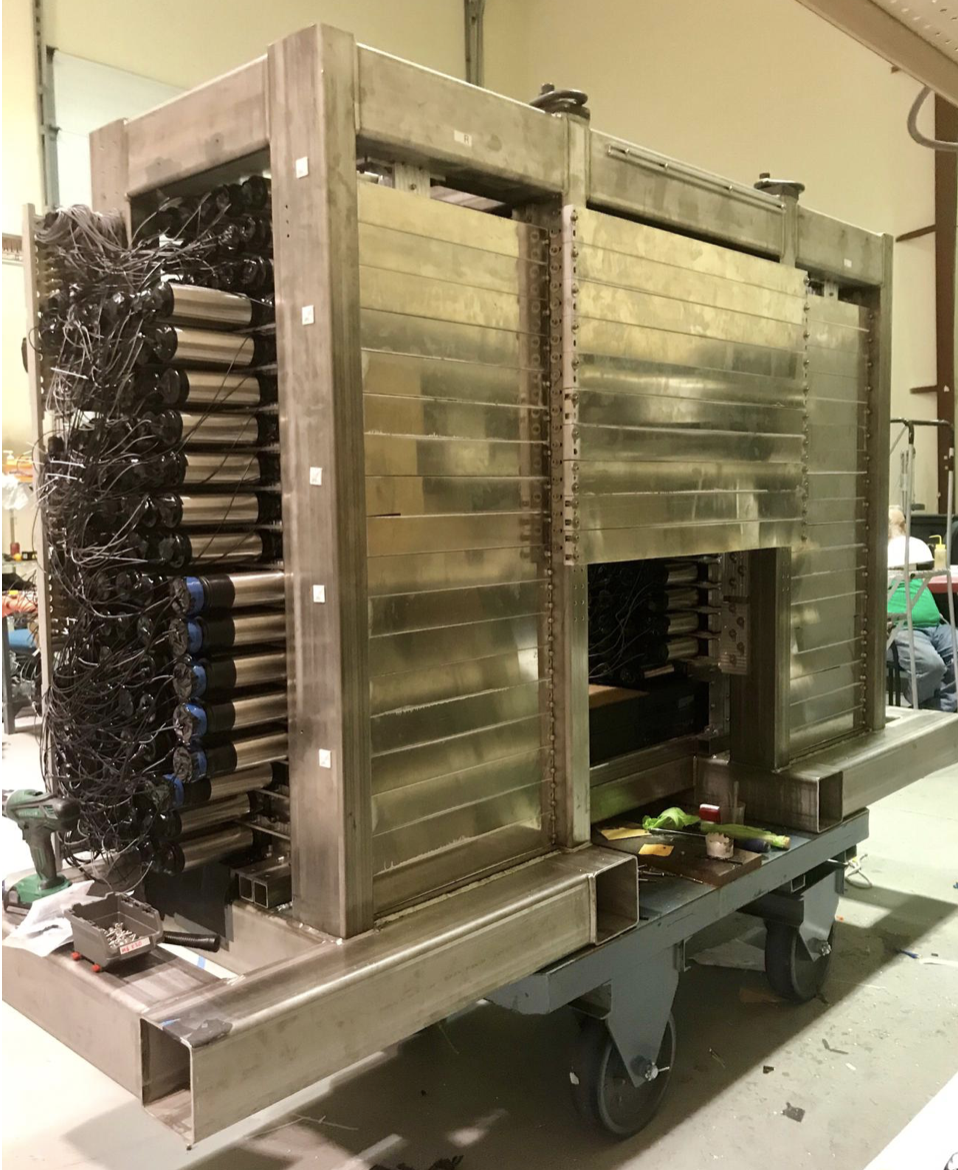
\includegraphics[width=0.48\textwidth]{band_pre.png}
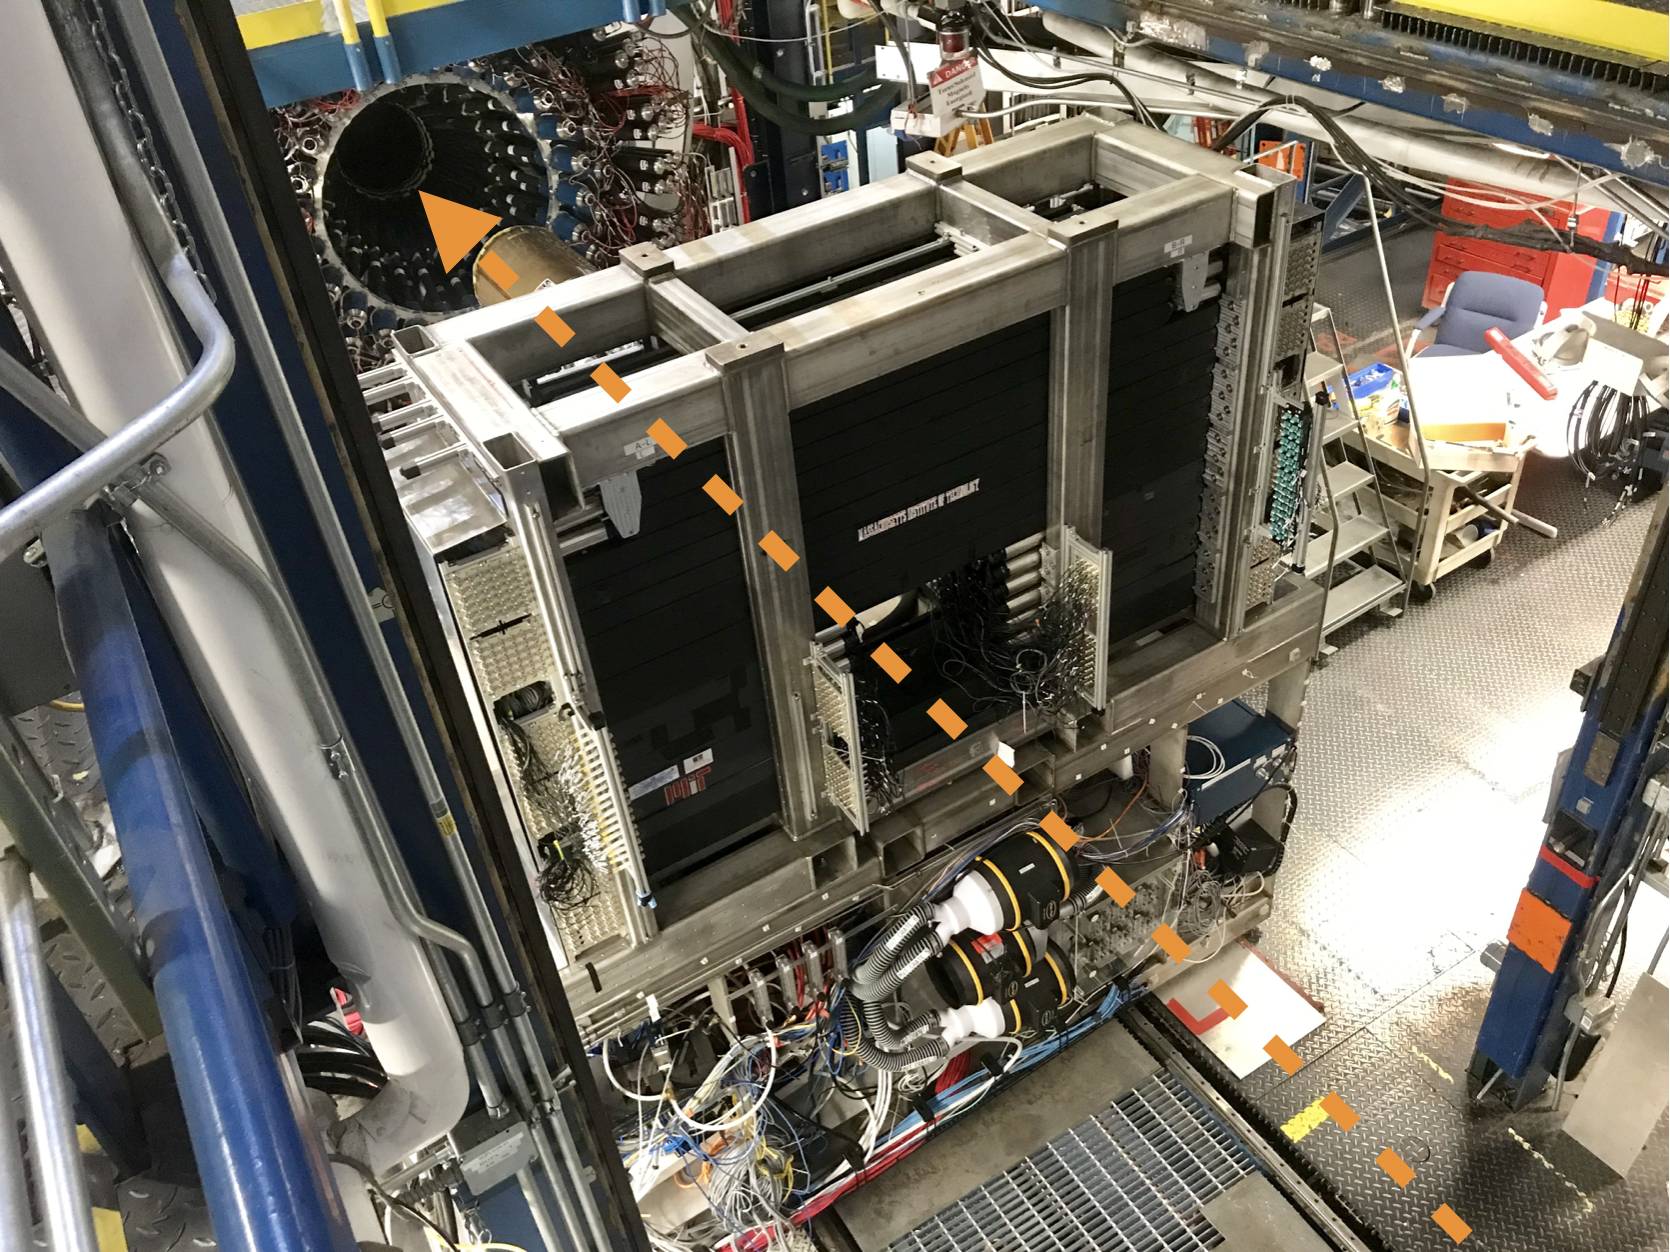
\includegraphics[width=0.48\textwidth]{band_hall1.png}
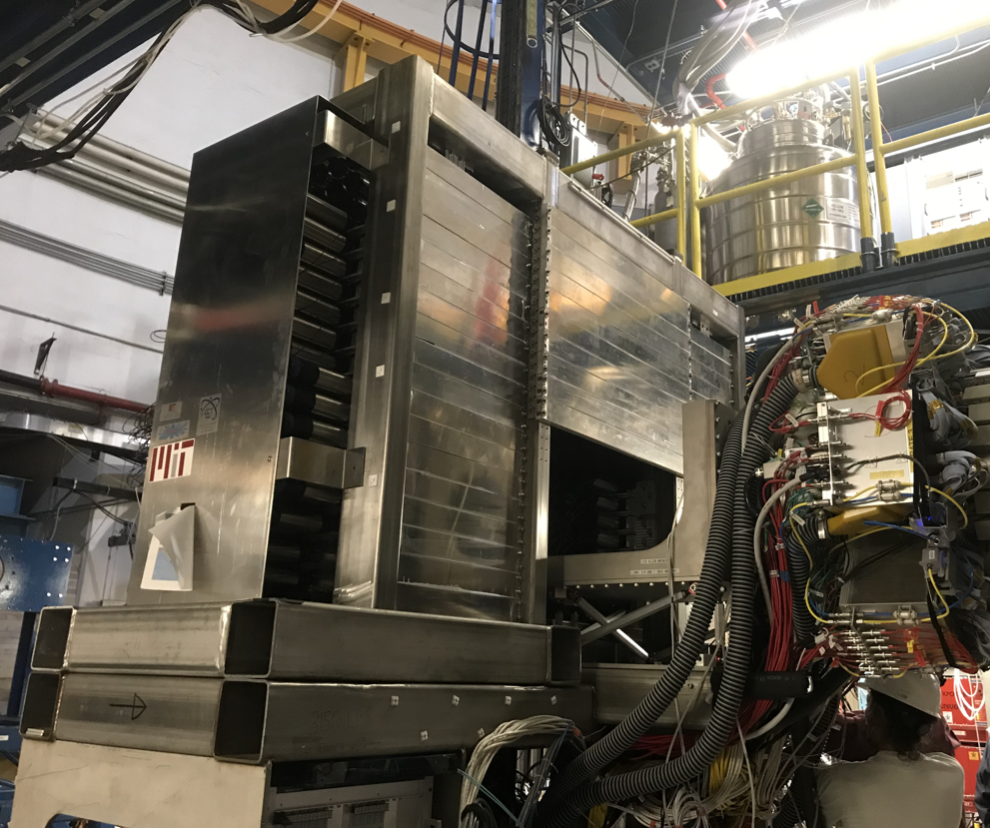
\includegraphics[width=0.48\textwidth]{band_hall2.png}
  \label{fig:bandcontext}
\end{figure}

The BAND detector consist of plastic scintillators made from  EJ-200 scintillant. Each bar in the active detector area has a cross section of $7.2 \times 7.2\,\mathrm{cm}^{2}$. In total there are 116 scintillator bars, arranged in 5 layers with 18 vertically stacked bar. The arrangement of the bars is shown in Fig. \ref{fig:barlayout}. The bottom rows are only arranged in four layers due to obstruction from surrounding frames.

\begin{figure}[htb]
\centering
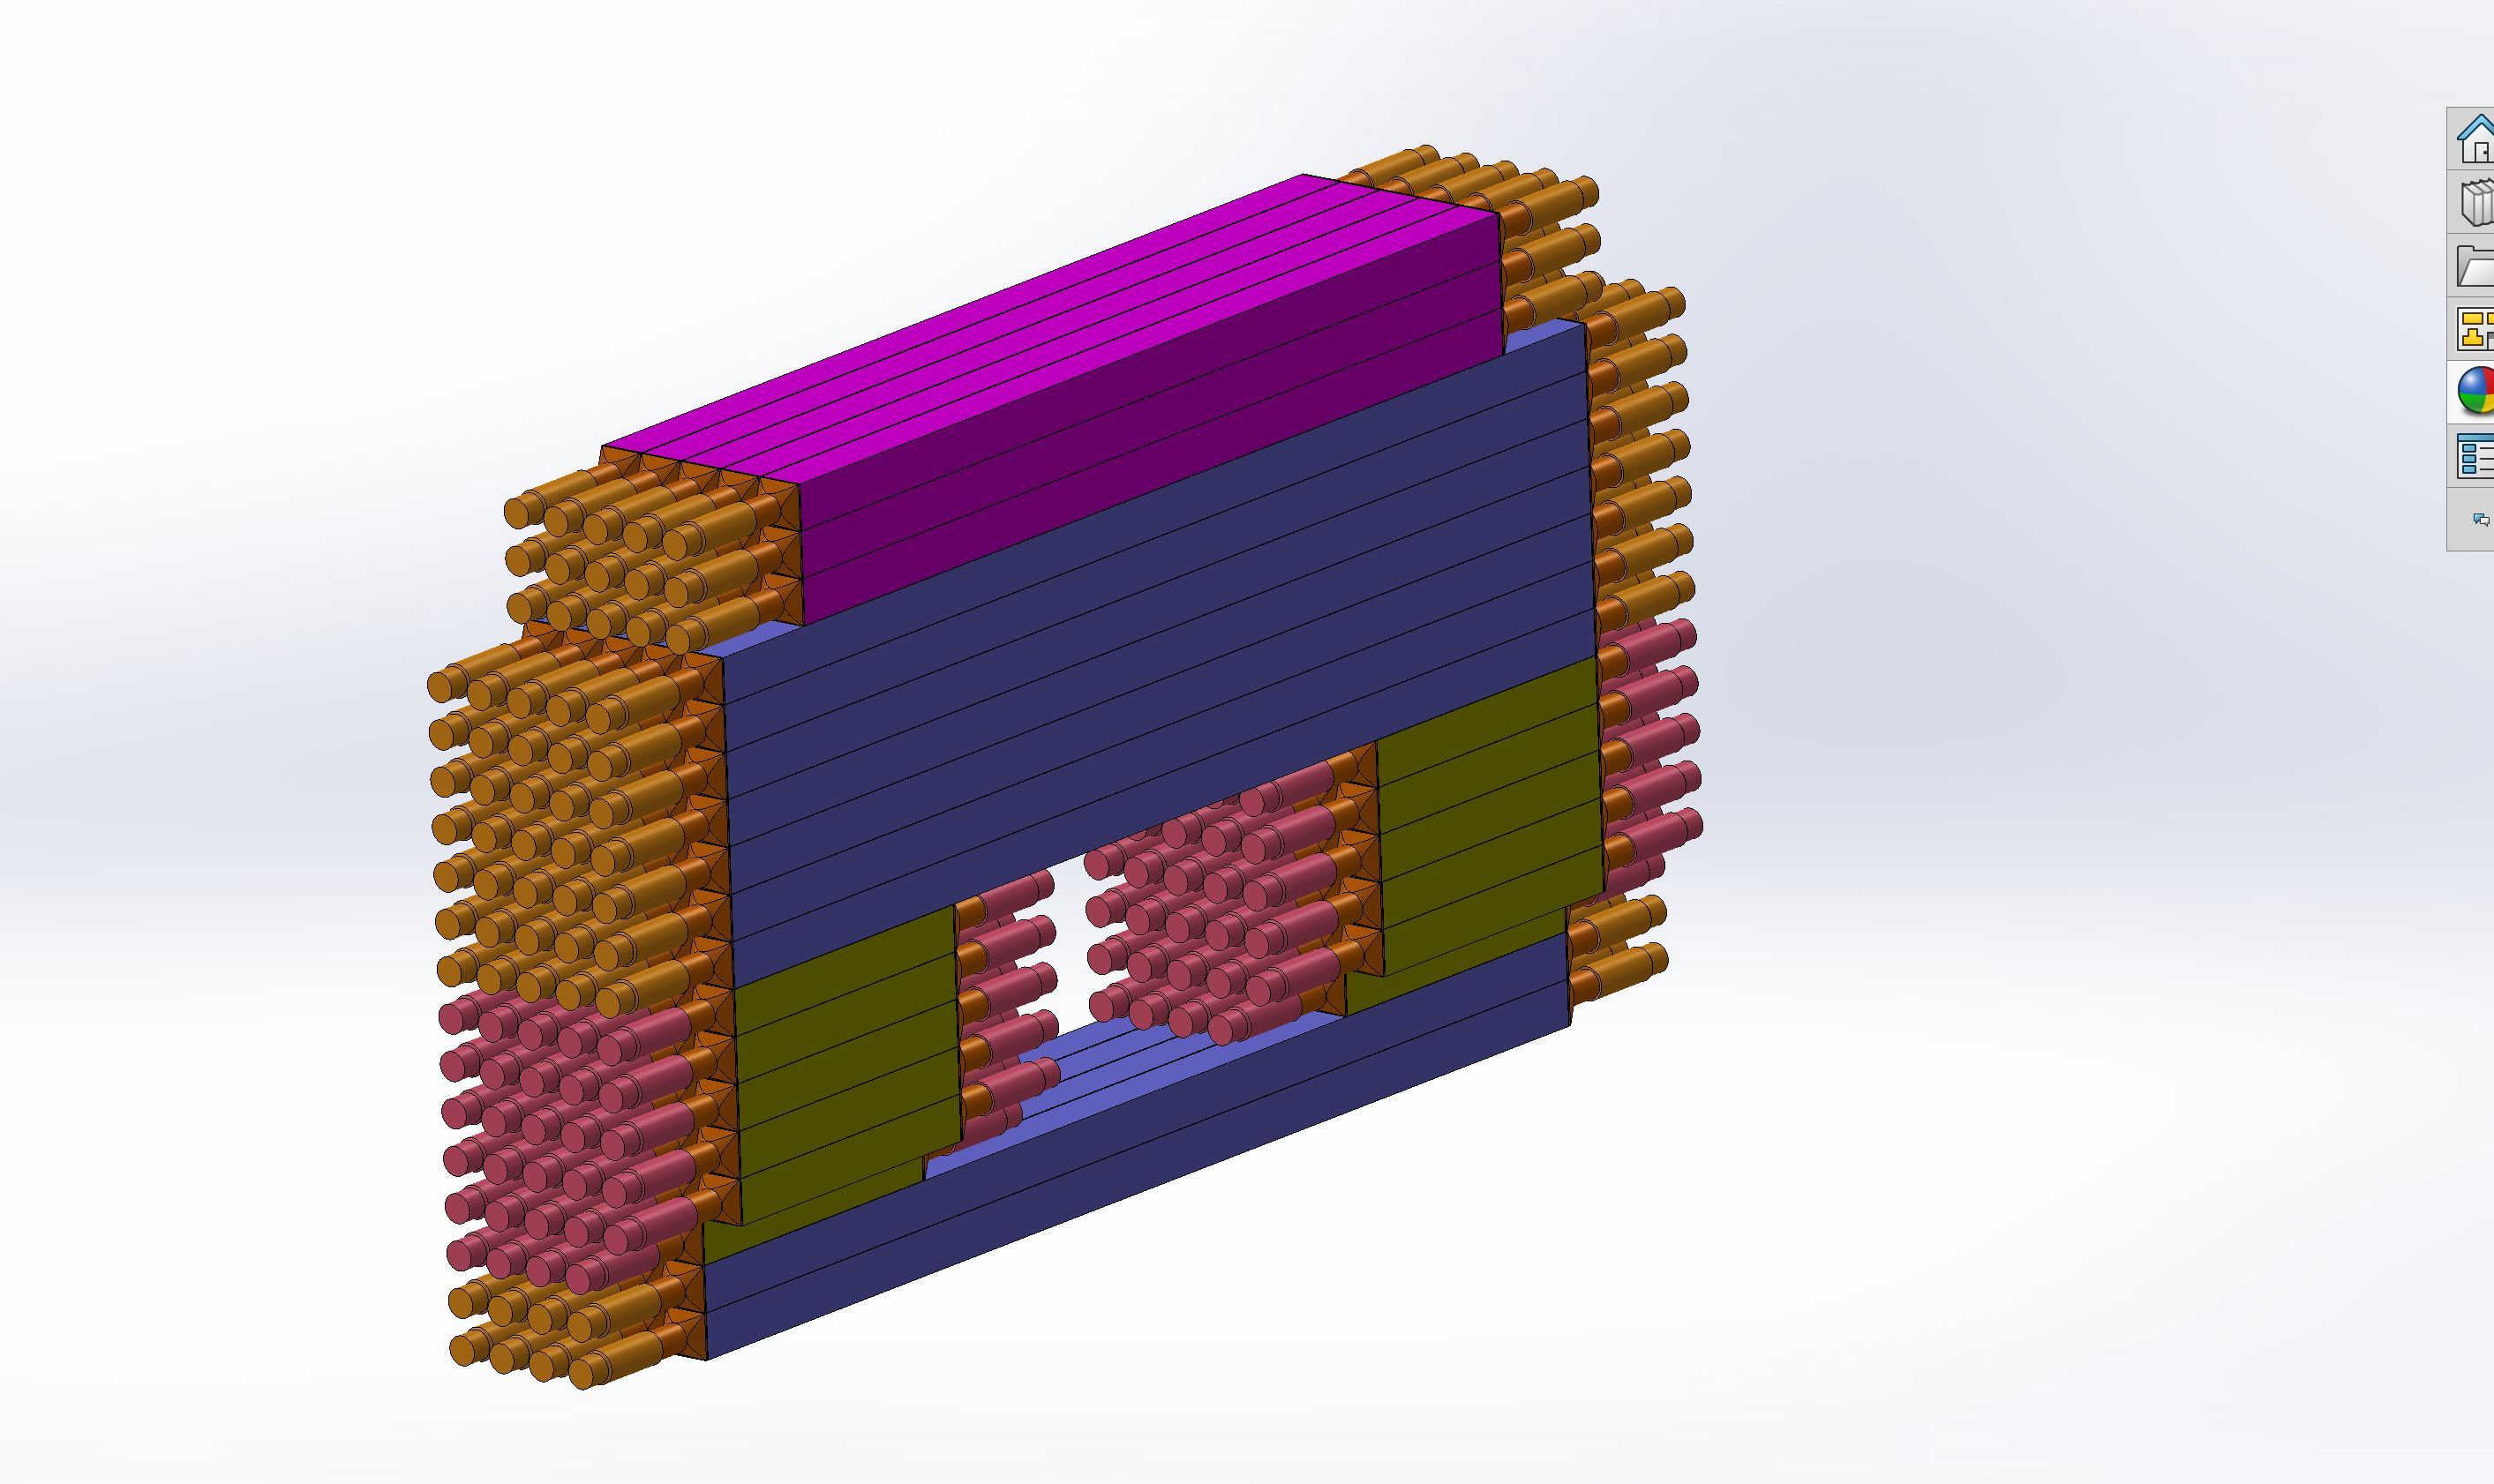
\includegraphics[width=0.48\textwidth]{Band01.png}
 \caption {(Left) Isometric view of the active BAND detector volume. The geometry is comprised of 5 layers of 18 vertically stacked bars. The magenta bars (top) are $164\,\mathrm{cm}$ long, the blue bars are $202\,\mathrm{cm}$ long while the shorter green bars around the beam hole are $51\,\mathrm{cm}$ long. Every bar is read out on both sides by a PMT. (Right) Isometric view of the BAND veto layer. It is similar to the active area of BAND. The bars have the same length as the bars shown in Fig. \ref{fig:barlayout}. Every bar is read out on one side by a PMT.}
  \label{fig:vetolayout}
\end{figure}
Three different long bars are used in the detector: 15 bars with a length of $164\,\mathrm{cm}$ (magenta in Fig. \ref{fig:barlayout}), 43 bars with a length of $202\,\mathrm{cm}$ (blue in Fig. \ref{fig:barlayout}) and 58 short bars with a length of $51\,\mathrm{cm}$ (green in Fig. \ref{fig:barlayout}). The short bars are necessary for the hole for the beam line and target installation. The total thickness is $36\,\mathrm{cm}$ gives a neutron detection efficiency of about 30\%.

All bars are read-out on both sides by PMTs (100 Hamamatsu R7724  [ADD REF] and 132 ET 9214  [ADD REF]) giving a total of 232 active channels. Since the PMTs are placed in the fringe field region of the solenoid, and they are encased in a cylindrical shielding made up by a \SI{2}{\milli\metre} thick layer of mu-metal.

In front of the first active layer of BAND, a veto layer is installed with 24 scintillators bars which are read-out only on one side by Thorne EMI 9954KB PMTs [ADD REF]. The bars have a cross section of $2 \times 7.2\,\mathrm{cm}^{2}$. The bars in the veto layer have the same length as the bars of one layer of the active detector area. The veto layer is shown in Fig. \ref{fig:vetolayout}.

\item Scint material
\item which PMTs / why
\begin{figure}[h!]
\centering
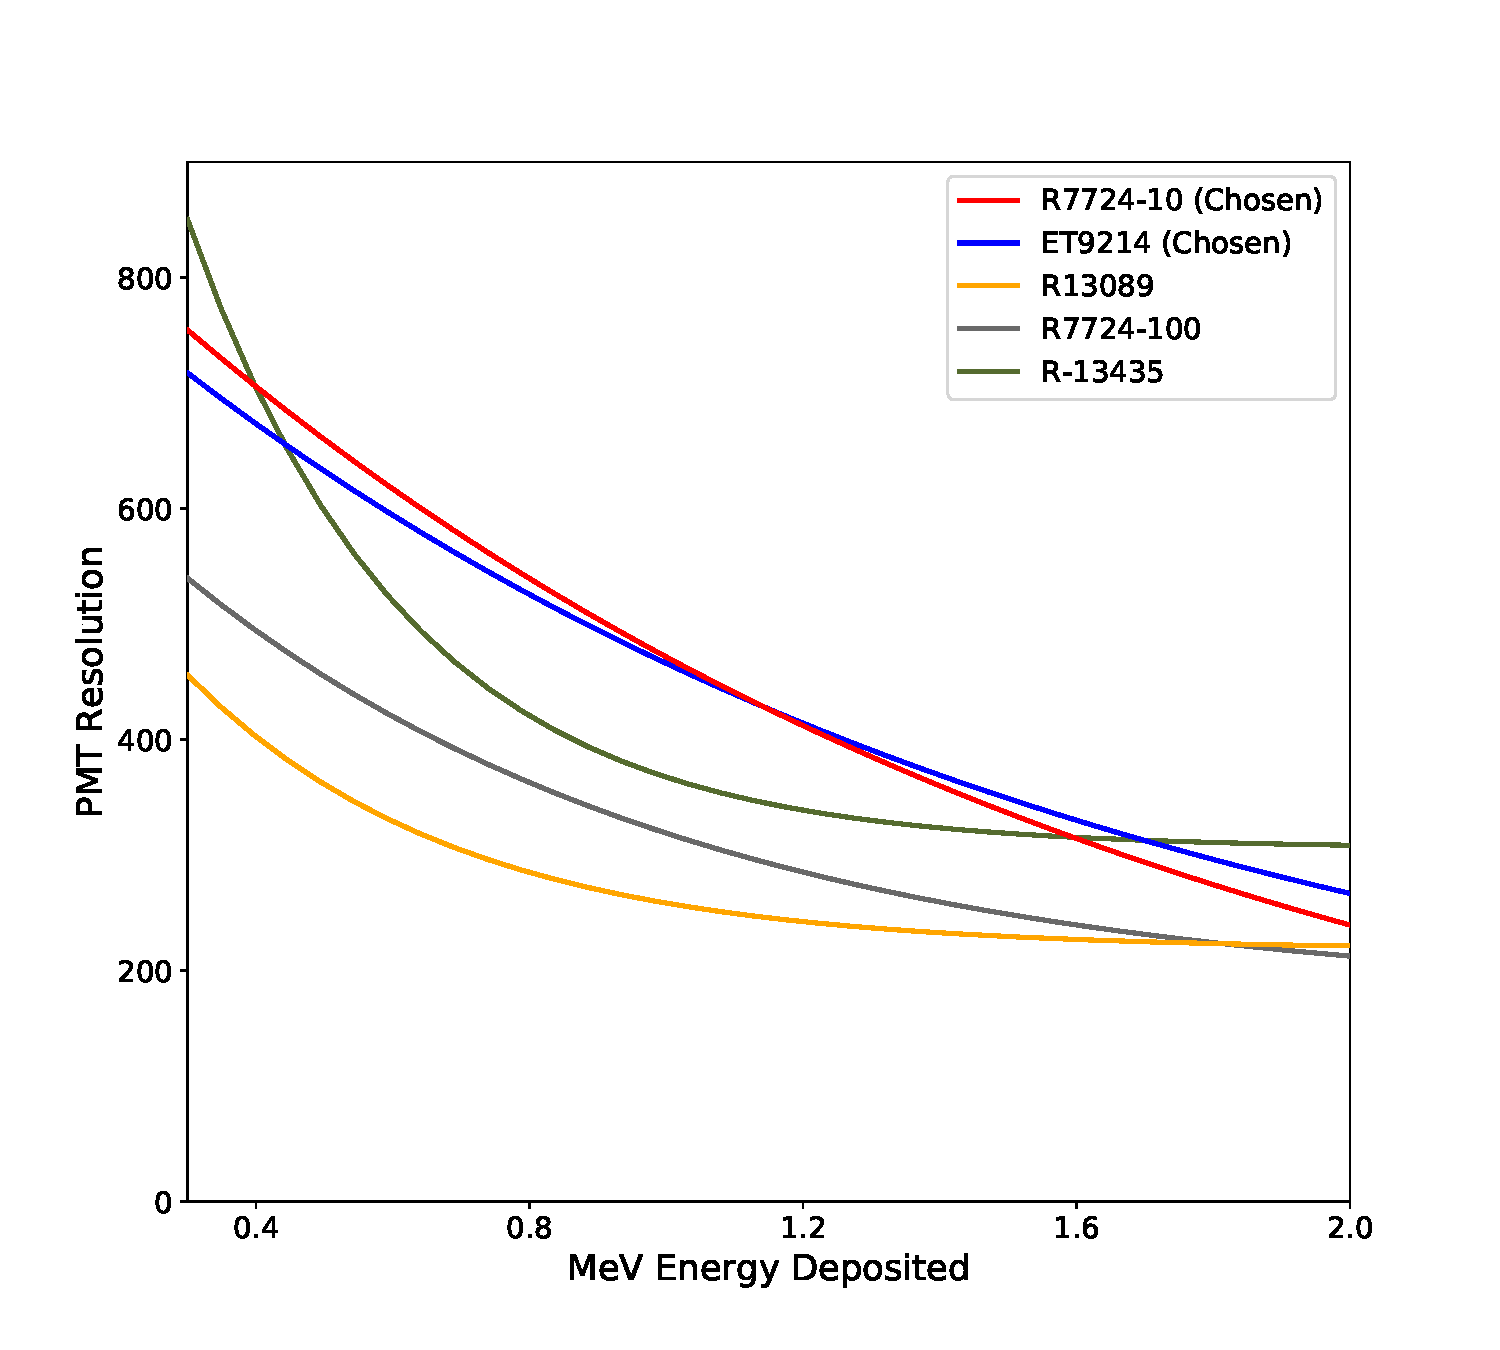
\includegraphics[width=0.7\textwidth]{test-stand/test-resolutions.pdf}
\caption{}
\label{fig:bandpmts}
\end{figure}

\item mu metal study
\item light guides
\begin{figure}[h!]
\centering
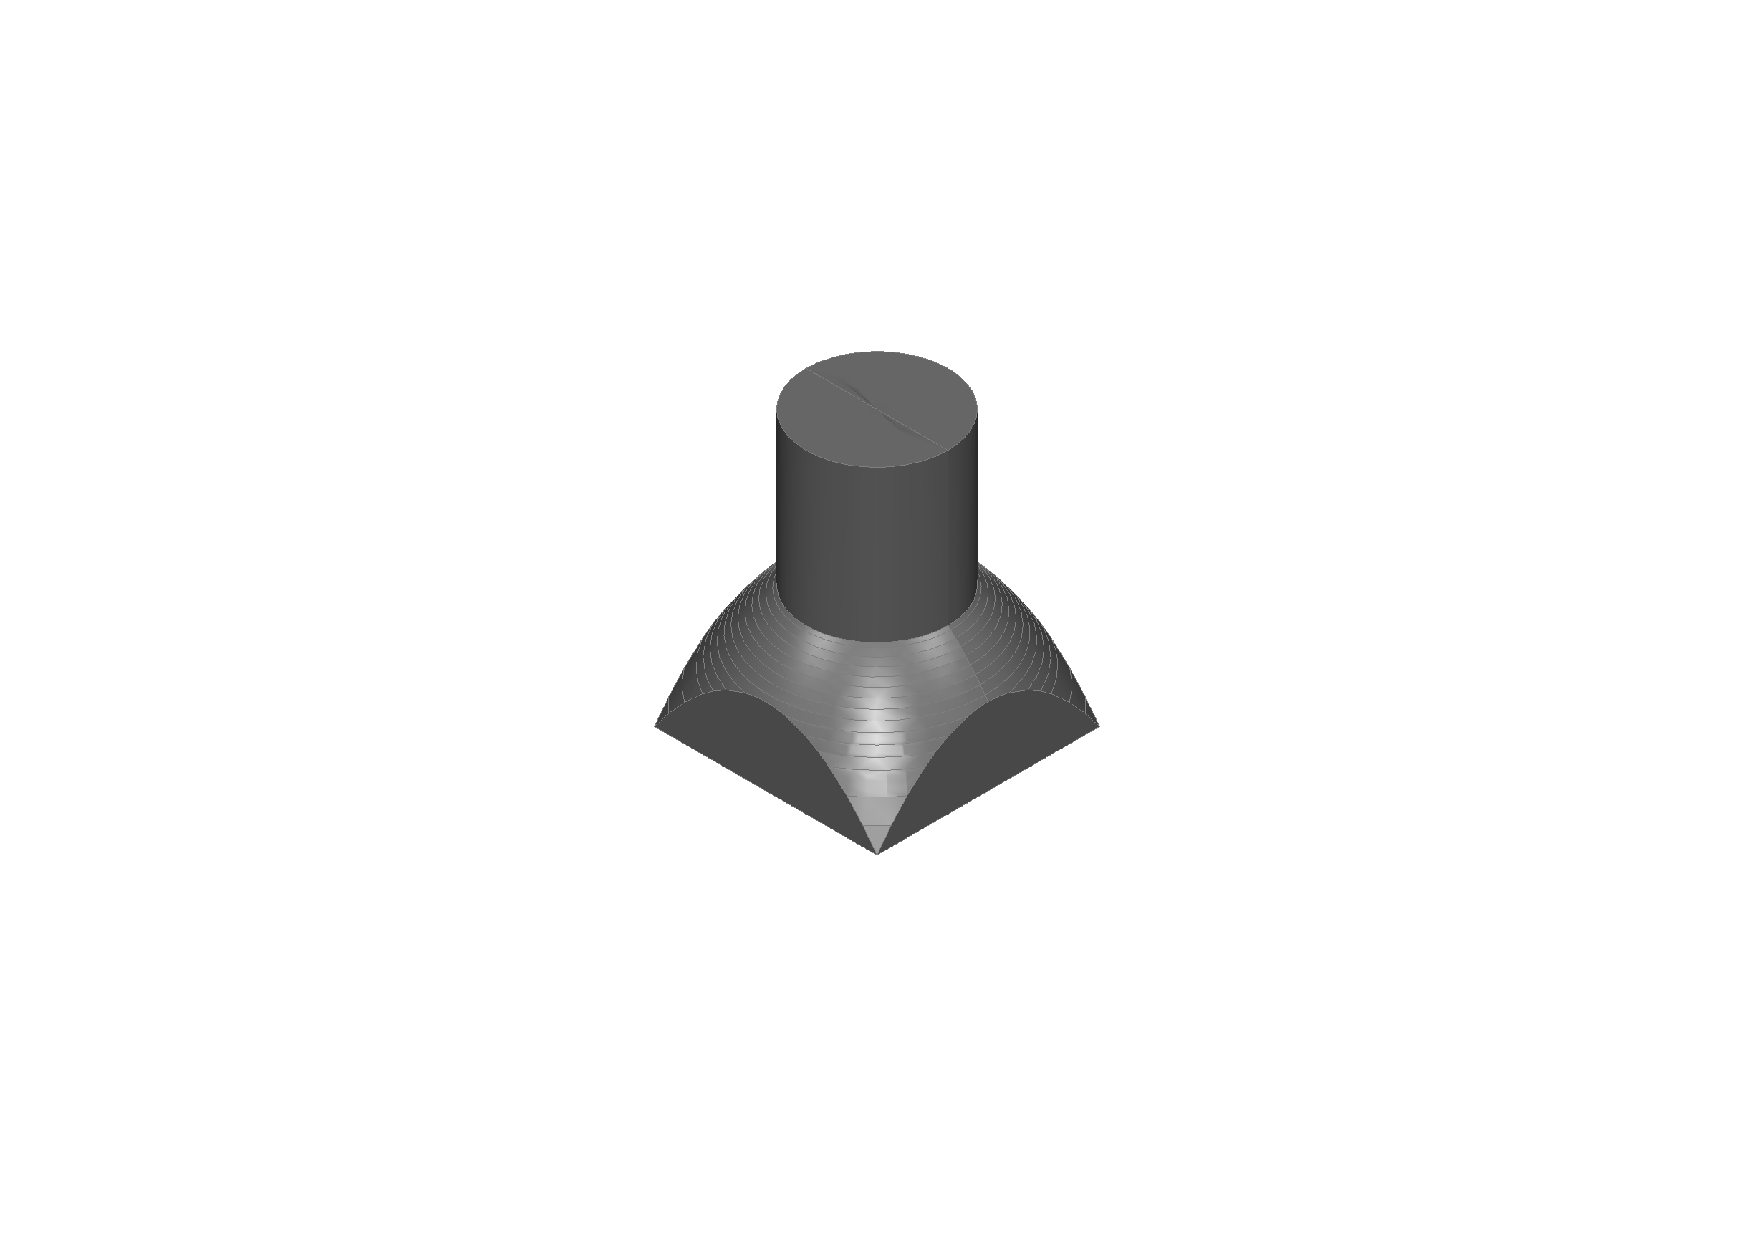
\includegraphics[width=0.45\textwidth]{parts/bar_lg.pdf}
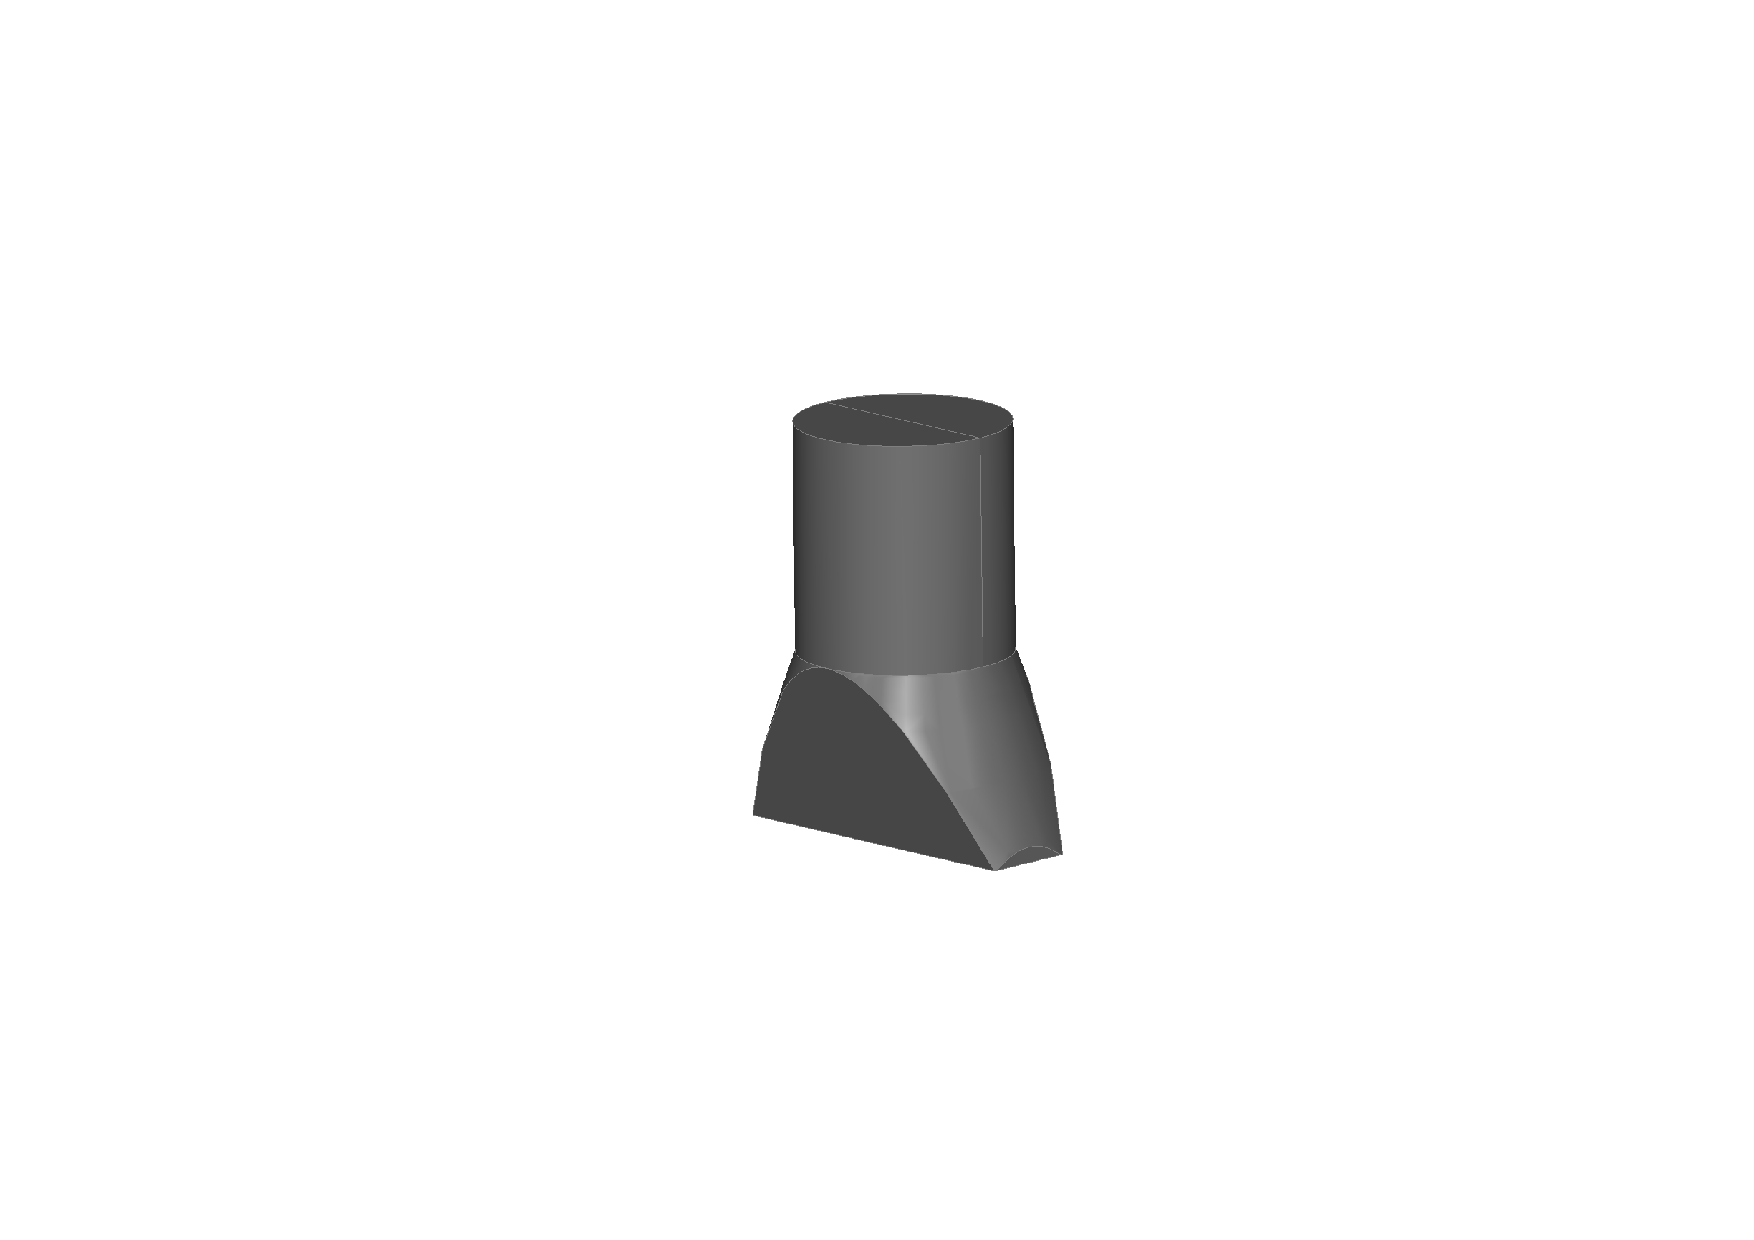
\includegraphics[width=0.45\textwidth]{parts/veto_lg.pdf}
\caption{}
\label{fig:bandlg}
\end{figure}

\item assembly, installation
\item electronics
\begin{figure}[h!]
\centering
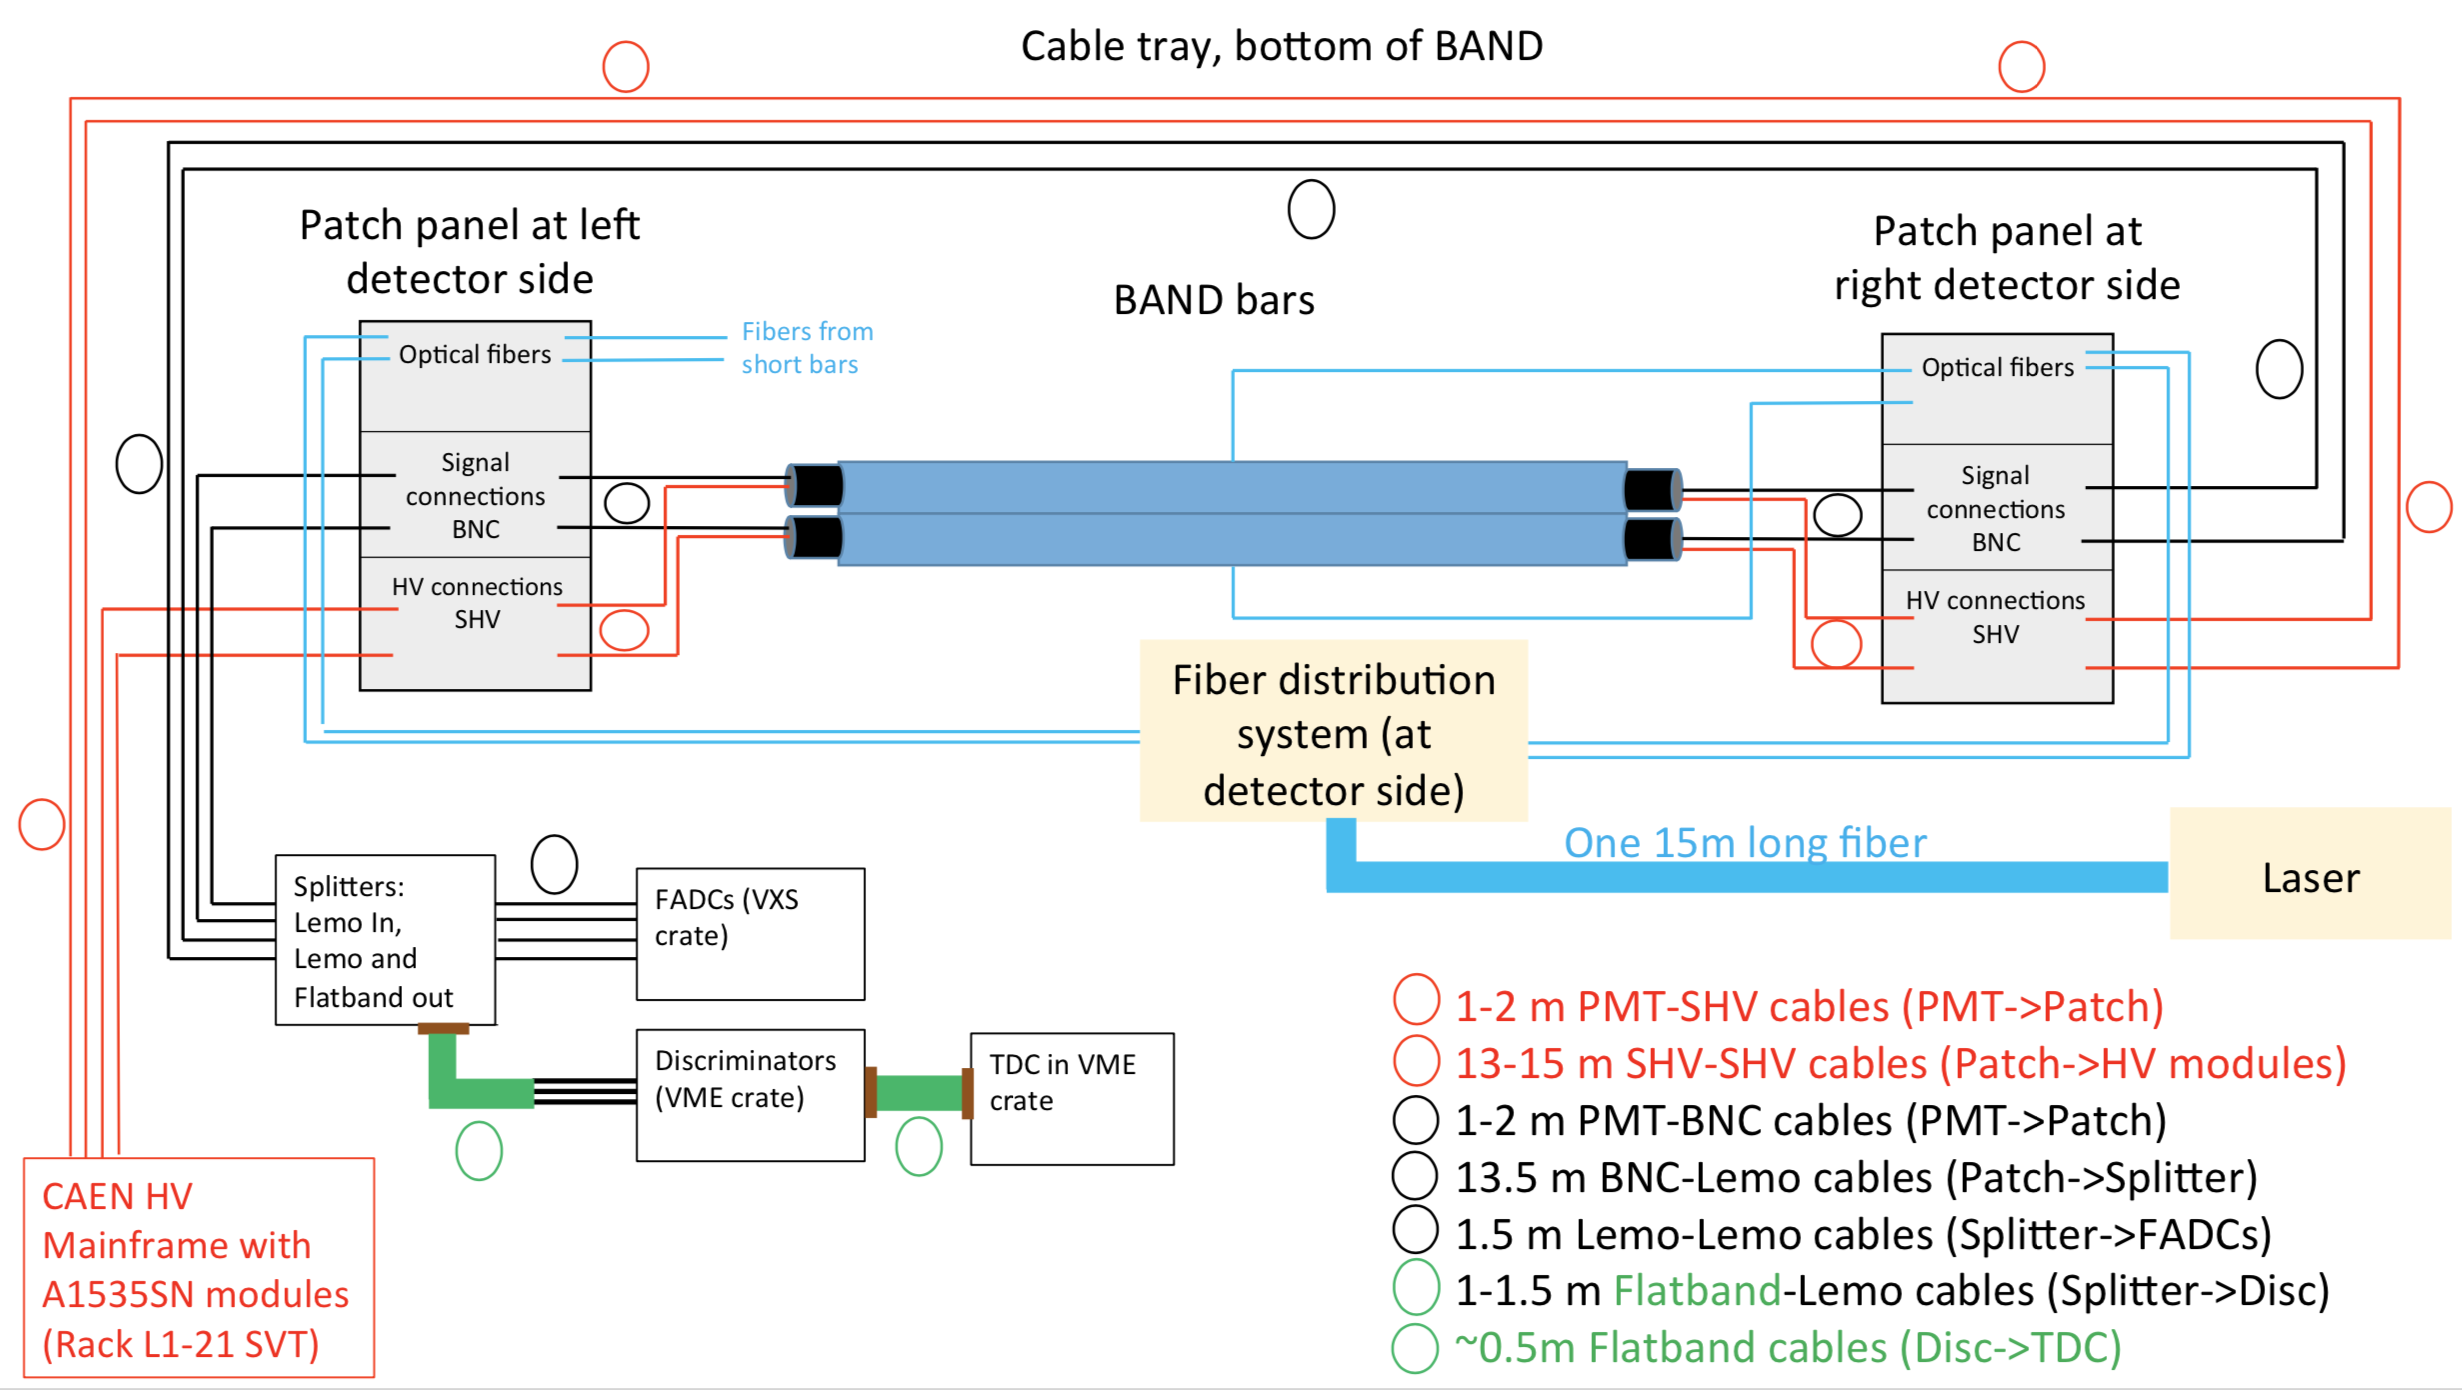
\includegraphics[width=0.8\textwidth]{figures/layout.png}
\caption{}
\end{figure}

The total number of channels for BAND including the veto layer is 256. Between BAND and CLAS a $2\,\mathrm{cm}$ lead shield is installed.


In order to operate the PMTs, high voltages (typically in the range of 1500 V) are provided by a multi-channel CAEN SYS4527 mainframe with 11 A1535SN cards (24 channel each).
The signal of each PMT is sent to an splitter. The splitter are the same as the one used by the HPS experiment.
From the splitter one signal is sent to flash-ADCs (250 VXS, 16 channels/board, made and owned by JLab) while the other signal is sent to  discriminators used by HPS (16 channels/board).
The discriminated time signal then goes to a TDC (CAEN VX1190A, 128 channels/board, 100 ps/channel resolution). The read-out system is installed left of BAND in beam direction. 
In total, the system consists of 16 flash-ADCs in one VXS crate, 16 discriminators and a TDC in a VME crate and 16 splitters.  Furthermore, a signal distribution card for the flash-ADCs and trigger interface boards are installed in the crates. A trigger for cosmics for testing and on a pulser for the laser calibration system will be implemented. BAND does not need to be implemented in the main event triggers of CLAS12.


\item laser system
The Laser calibration system consists of a Teem Photonics STV-01E-140 picosecond laser with a wavelength of $355\,\mathrm{nm}$, several splitters, reference photodiode and a fiber distribution system. All of these components are in a sealed, light-tight box. The output of the laser is about $1\,\mu\mathrm{J}$ which will be attenuated and distributed to all fiber outputs which have an output of about $100\,\mathrm{fJ}$. The fibers are connected via a patch panel to each scintillator bar. 
\begin{figure}[h!]
\centering
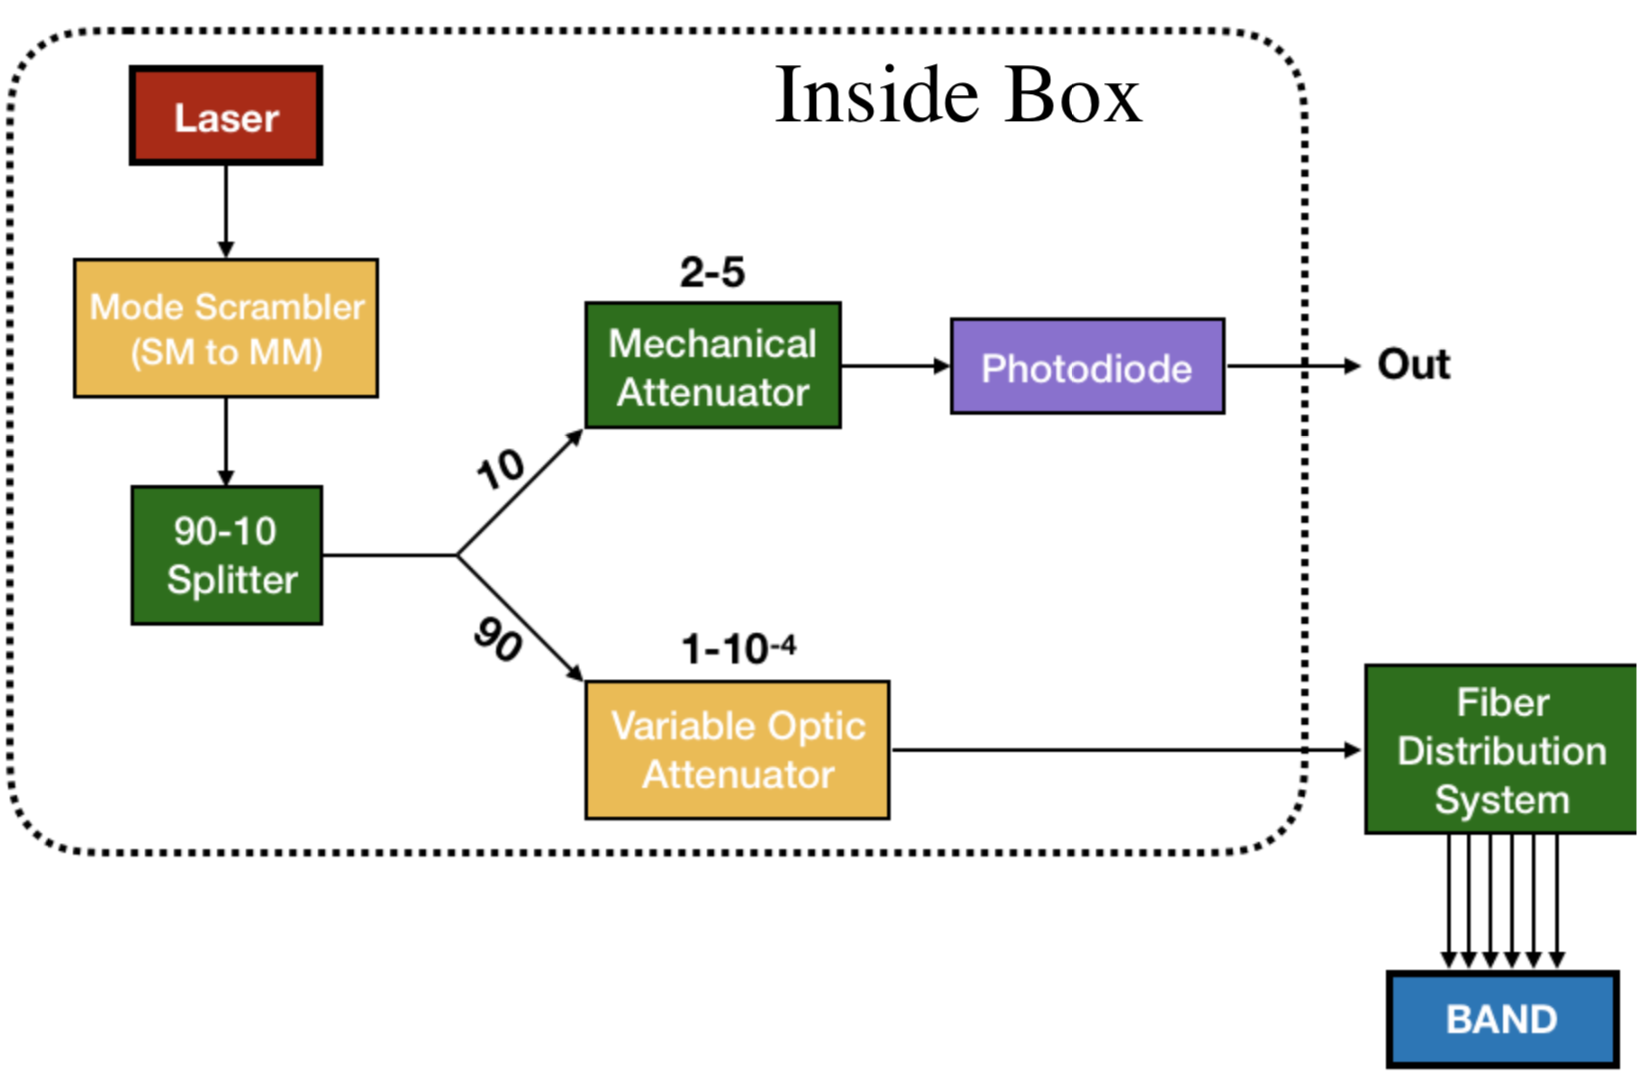
\includegraphics[width=0.8\textwidth]{figures/laser.png}
\caption{}
\end{figure}


\end{itemize}


% (E.S): I saw we can just quickly summarize the general design considerations in the intro, and leave these about more optimization of detector components and final design chosen
%NOTE: Not sure if this fits here, but the space constraints gave some limitation on the detector design.
%Due to space constraints in HallB, the only possible space closest to the target is on top of the support cart for the silicon vertex tracker of CLAS12.  The detector in context of its surroundings (target, beam line and cart) is shown in Fig. \ref{fig:bandcontext}.

%%%%%%%%%%%%%%%%%%%%%%%%%%%%%%%%%%%%%%%%%%%%%%%%%%%%%%%%%%%%%%%%%%%%%%%%%%%%%%%%%%%%%%%%%%%%%%%%%%%

\section{BAND Performance}

\begin{itemize}
\item bench measurements
Some plots from our most recent measurements in the lab with realistic BAND bars. Laser resolution and maybe a cosmic run.

\item source, cosmic, laser calibrations
\item beam performance
\end{itemize}

% ==================================================================================================
\subsection{Effective Velocity}
\begin{figure}[h!]
\centering
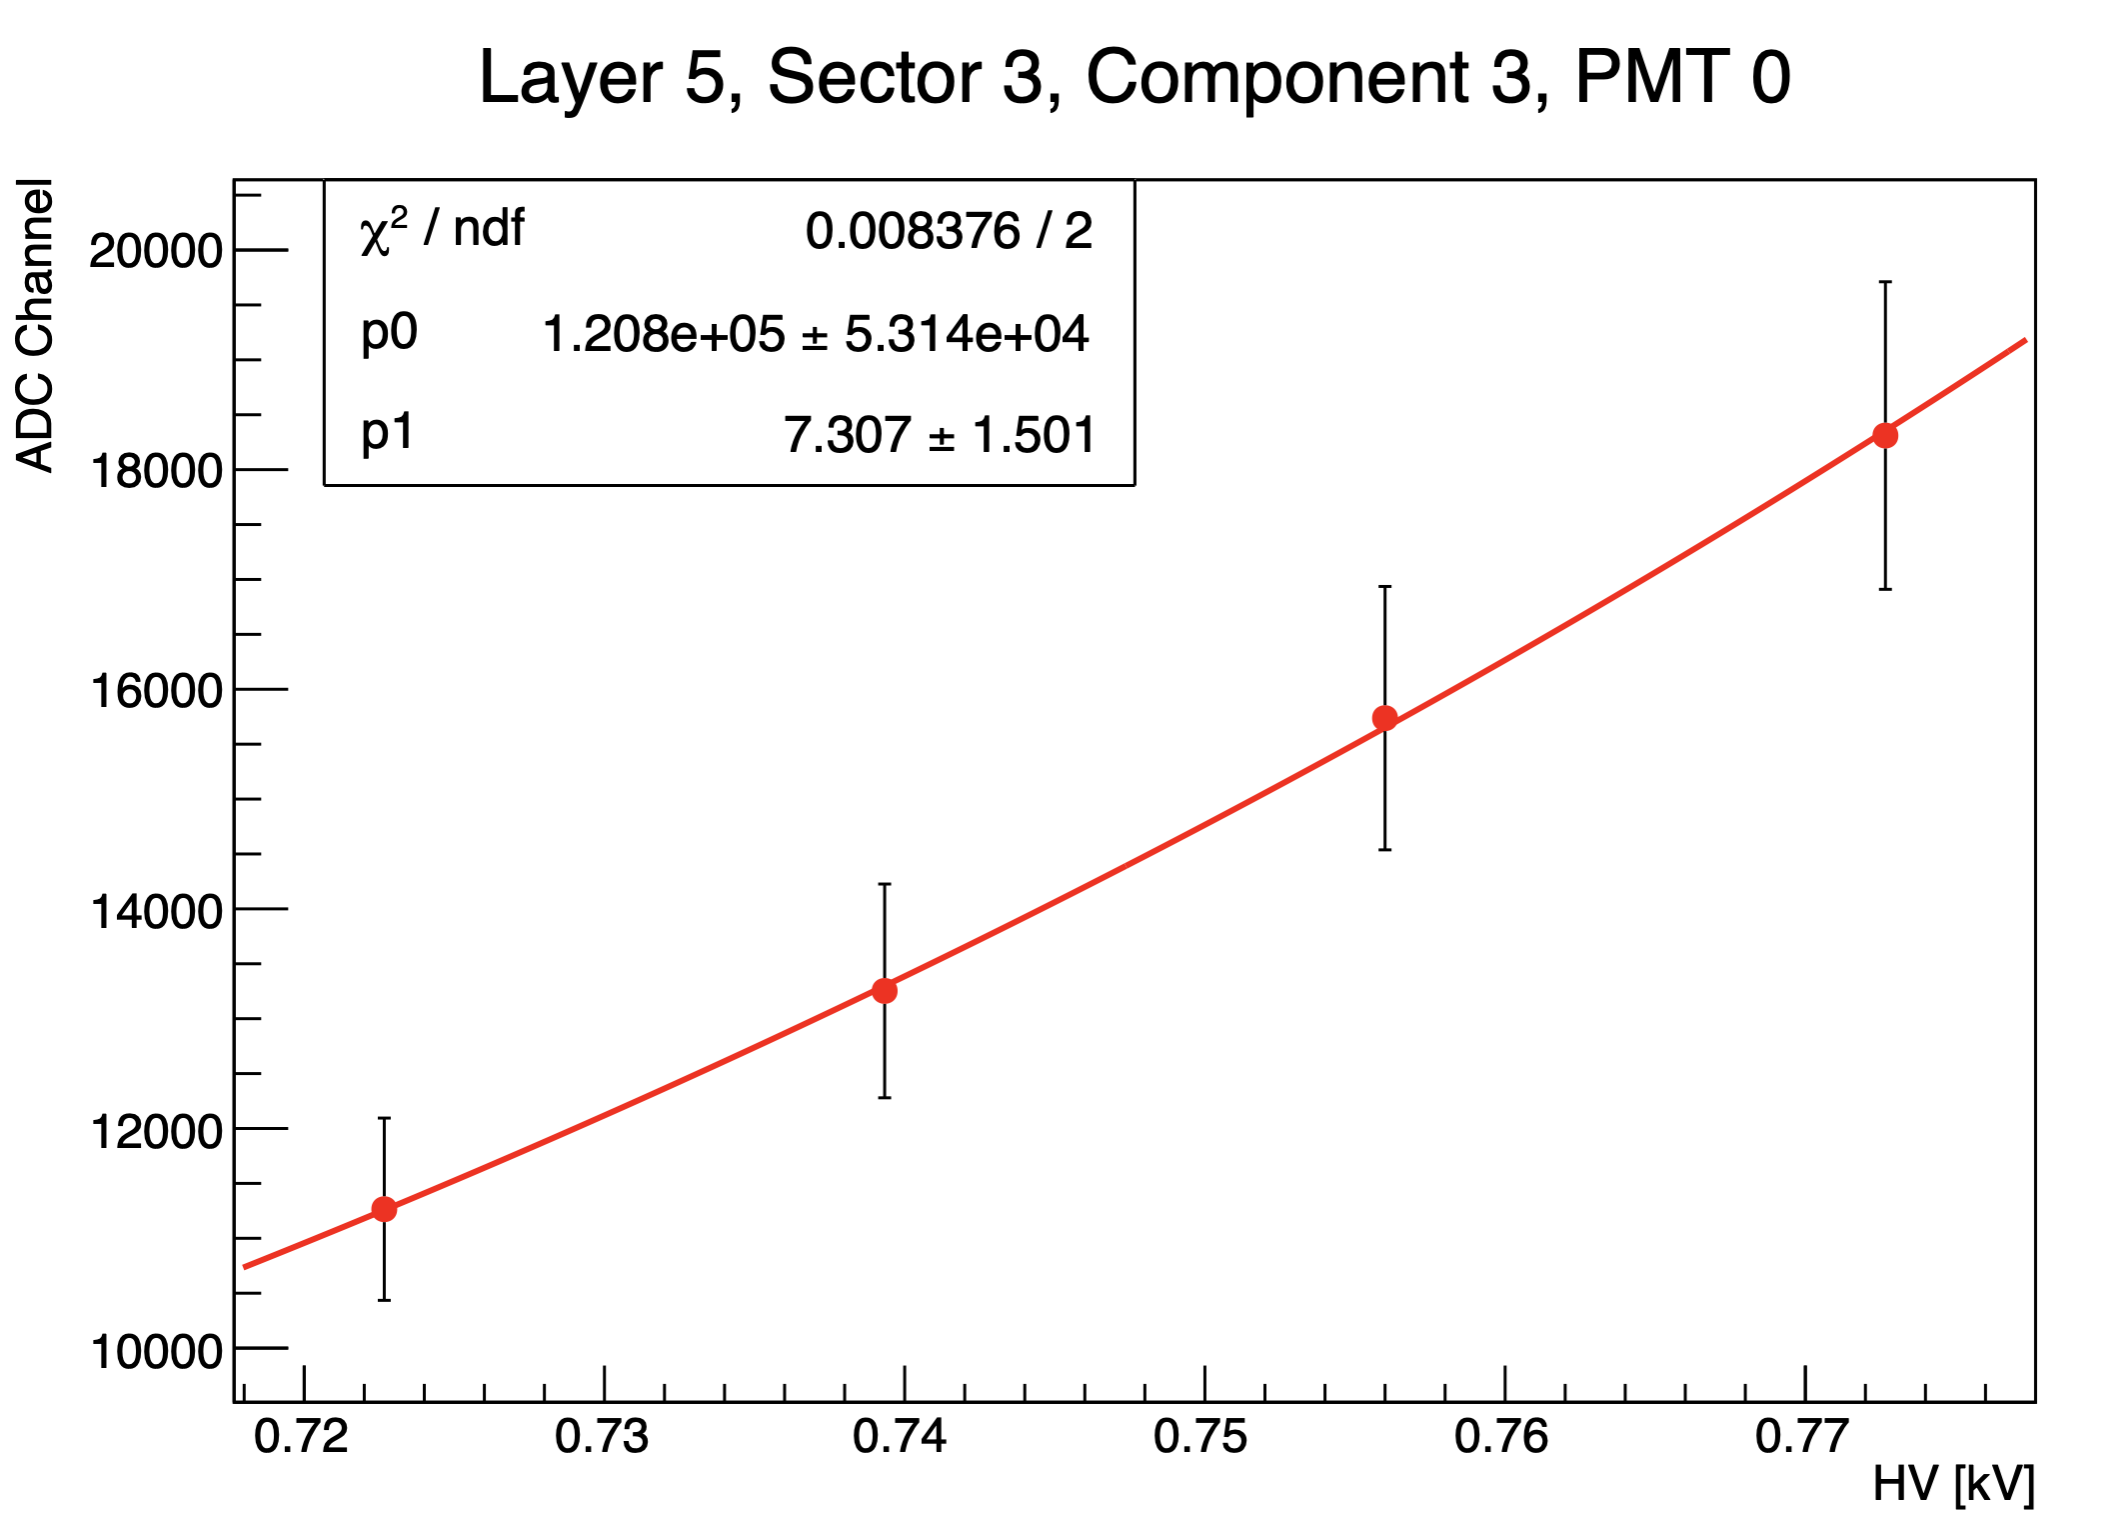
\includegraphics[width=0.8\textwidth]{figures/gainCurve.png}
\caption{}
\end{figure}

\begin{figure}[h!]
\centering
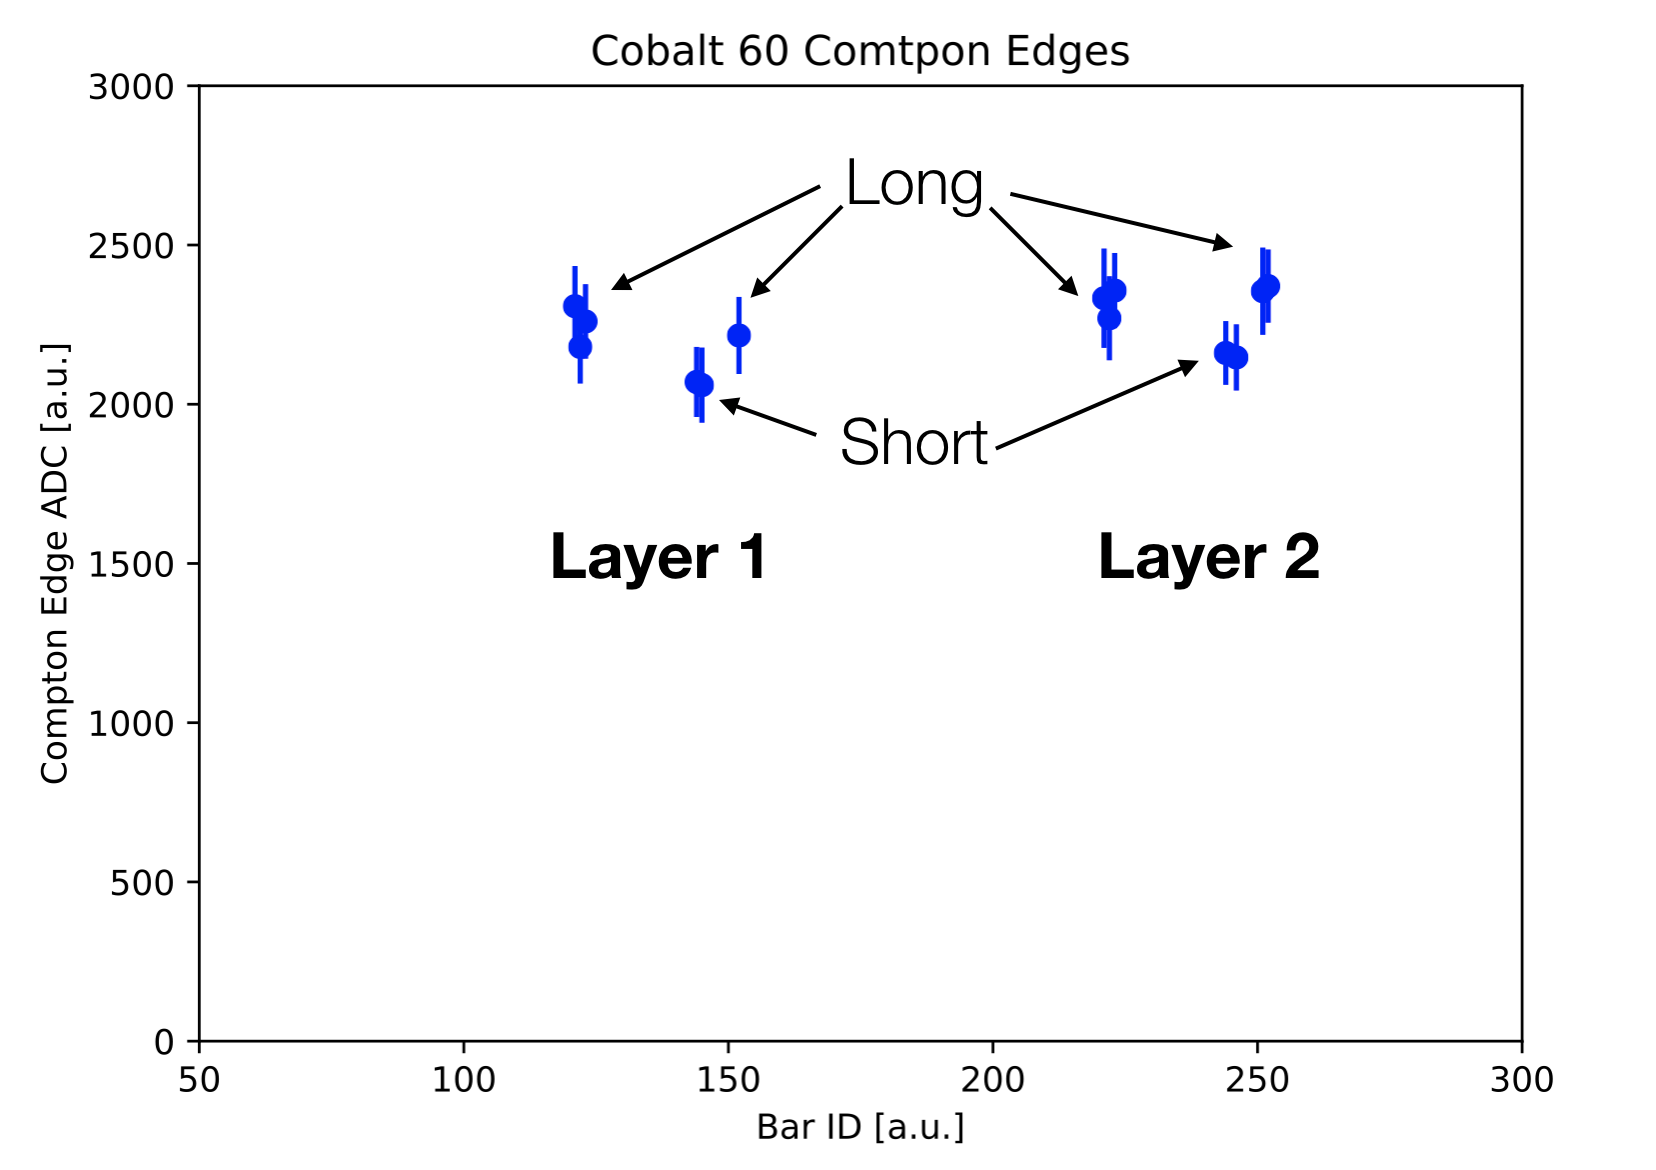
\includegraphics[width=0.8\textwidth]{figures/coedges.png}
\caption{}
\end{figure}



The velocity of light traveling through the scintillator bars 
can be determined from the width of the left minus right time spectra for a given bar ($\Delta t$), and the bar length ($L$) as:

\begin{equation}
v_{eff} = \frac{2 \cdot L}{\Delta t}
\end{equation}

% ---------------------------------------------------
\begin{figure}[h!]
\centering
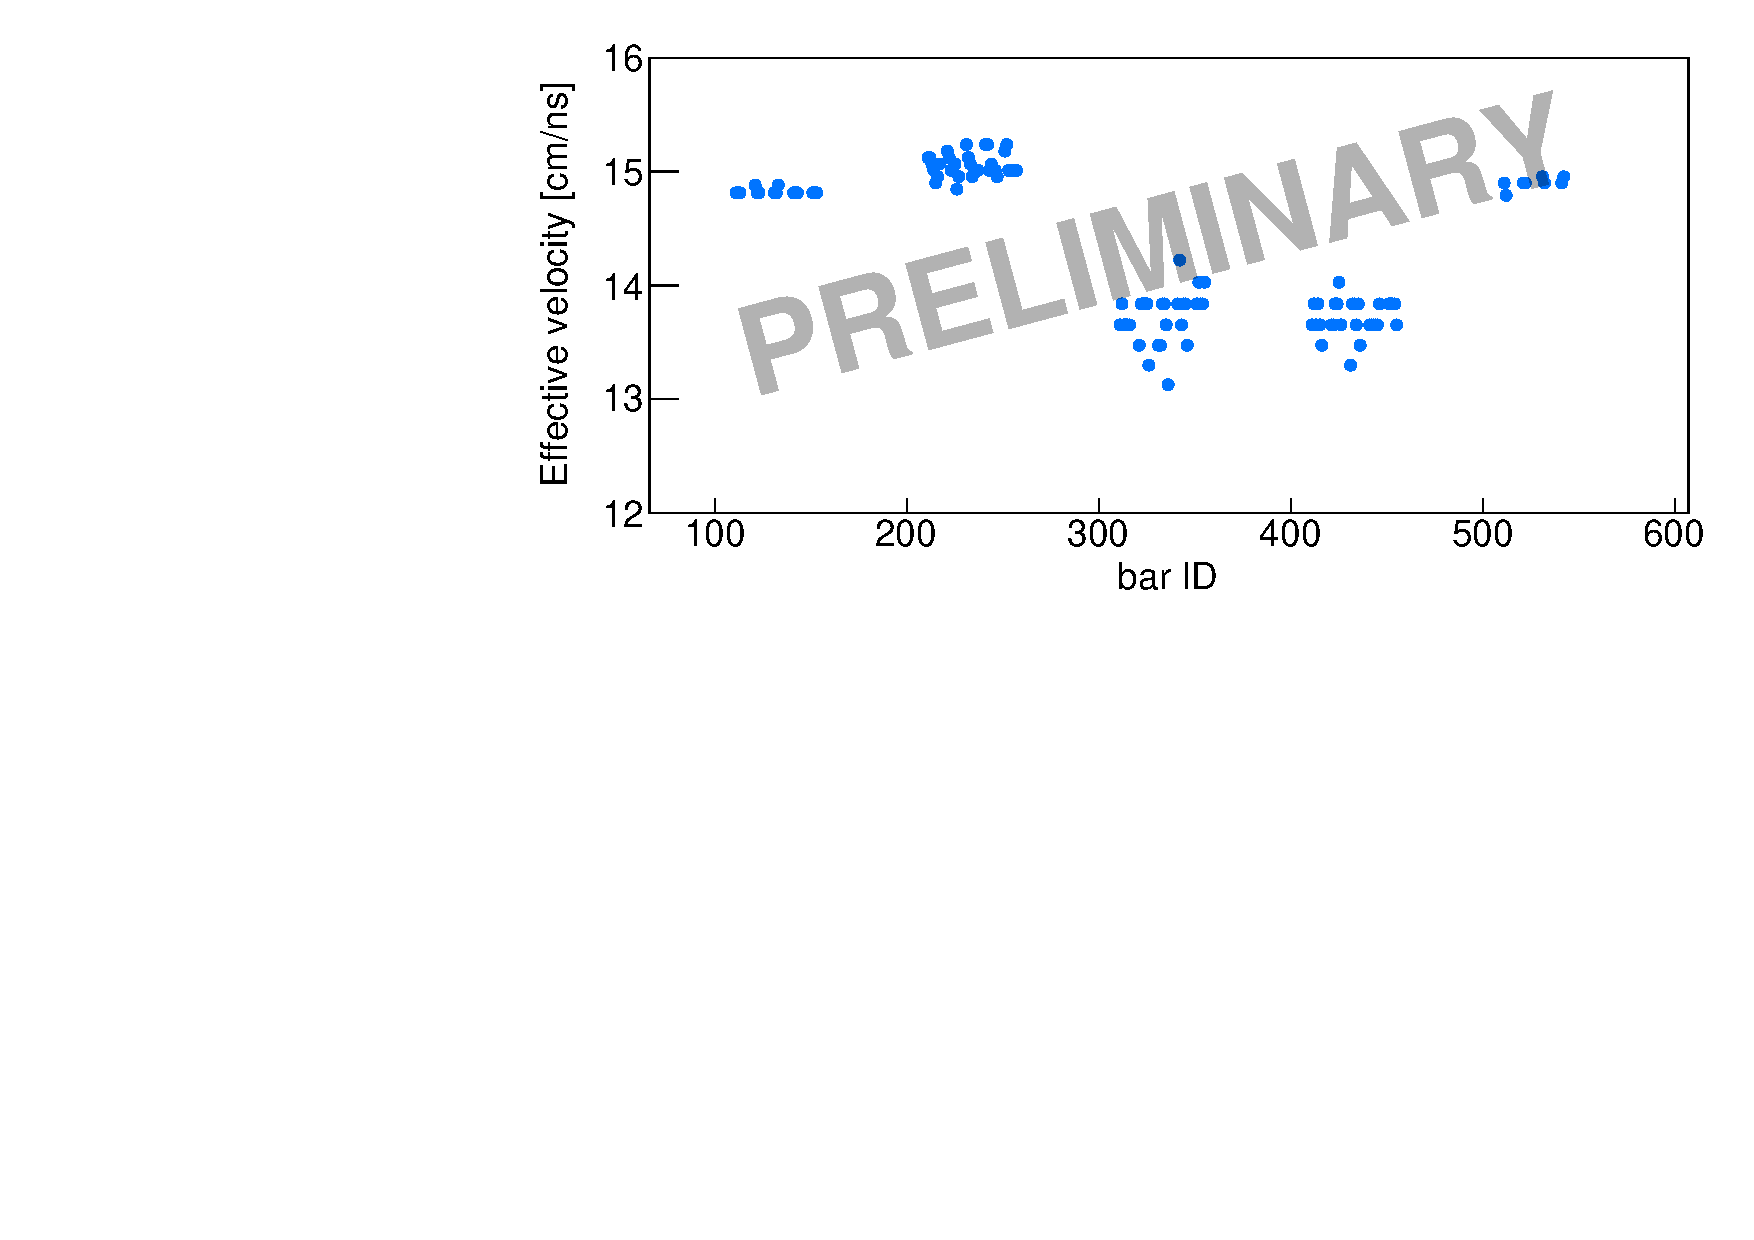
\includegraphics[width=0.8\textwidth]{figures/calibrations/eff_velocity.pdf}
\caption{}
\end{figure}
% ---------------------------------------------------

$\Delta t$ is defined as the the width of the left minus right time spectra at $20\%$ of the maximum of the distribution using cosmic data.

% ==================================================================================================
\subsection{Attenuation Length}

The distance in which the intensity of light traveling through a scintillator drops by $1/e$ is called attenuation length.
It is used to correct the ADC values when determining the deposited energy.
While scintillator manufacturers provide attenuation length values, this value can be significantly different
when a detector is built, and thus it has to me measured.
The attenuation length, hereby denoted by $\mu$, can be related to ADC and timing information recorded by
the left and right PMTs in a given bar as:

\begin{equation}
ln(R) \equiv ln \Big( \frac{\rm{ADC}_L}{\rm{ADC}_R} \Big) = -\frac{v_{eff}}{\mu}(t_L-t_R)
\end{equation}

Consequently, $\mu$ can be determined by fitting a linear function to a plot of $ln ( R )$ vs. $-v_{eff}(t_L-t_R)$
and extracting the inverse of the slope. We carry out this measurement with cosmic data, since cosmic rays
interact with the detector throughout the entire length of the bars (in contrast, for example, with the laser data,
which only produces hits at the center of the bar).

\begin{figure}[h!]
\centering
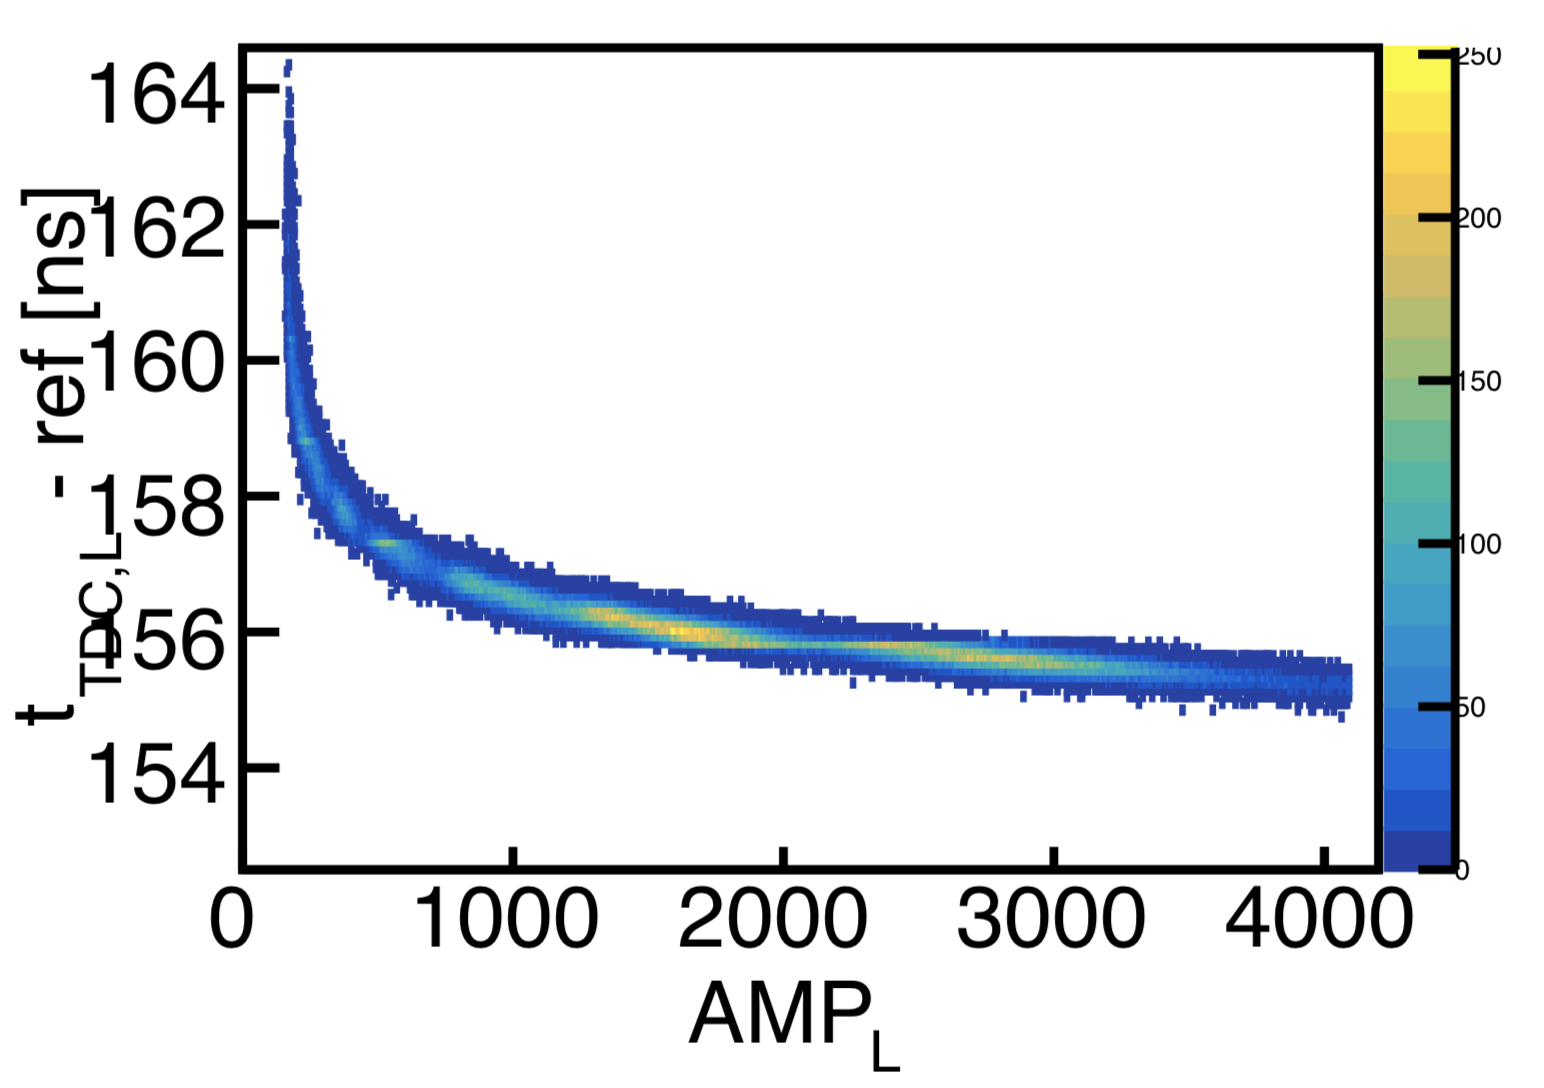
\includegraphics[width=0.8\textwidth]{tw_before.png}
\caption{}
\end{figure}
\begin{figure}[h!]
\centering
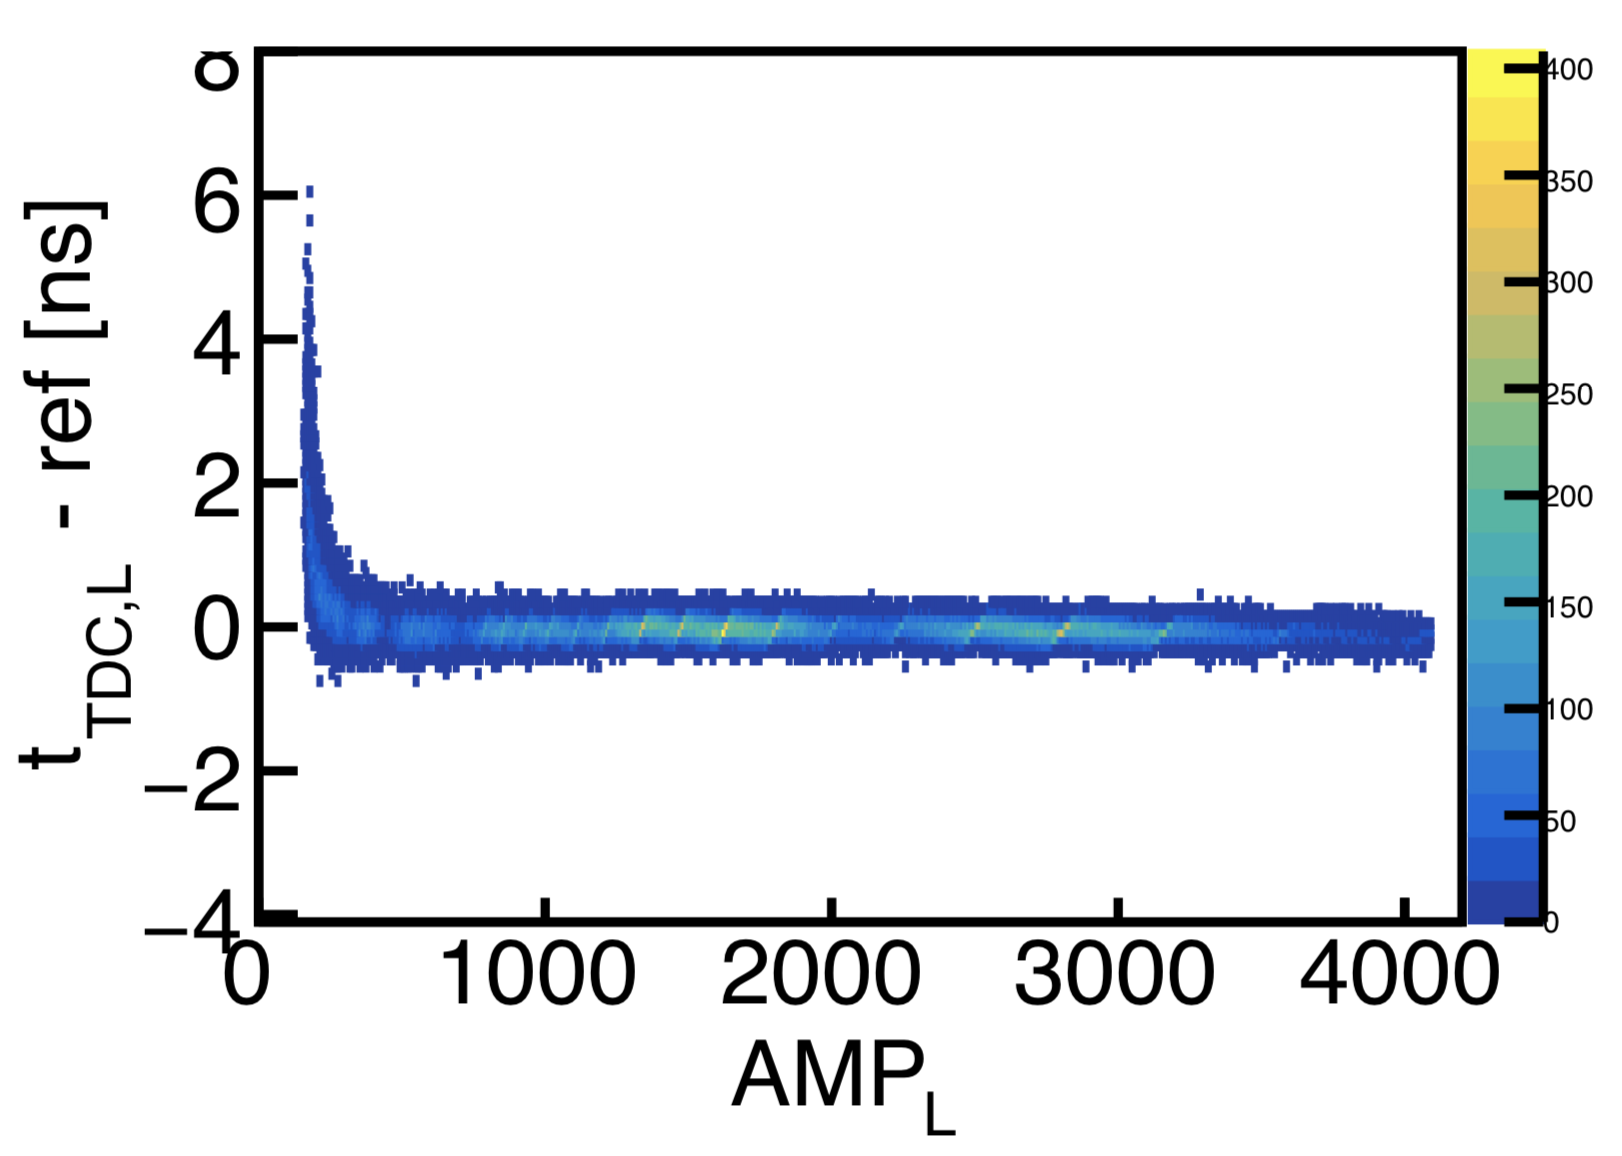
\includegraphics[width=0.8\textwidth]{tw_after.png}
\caption{}
\end{figure}

\begin{figure}[h!]
\centering
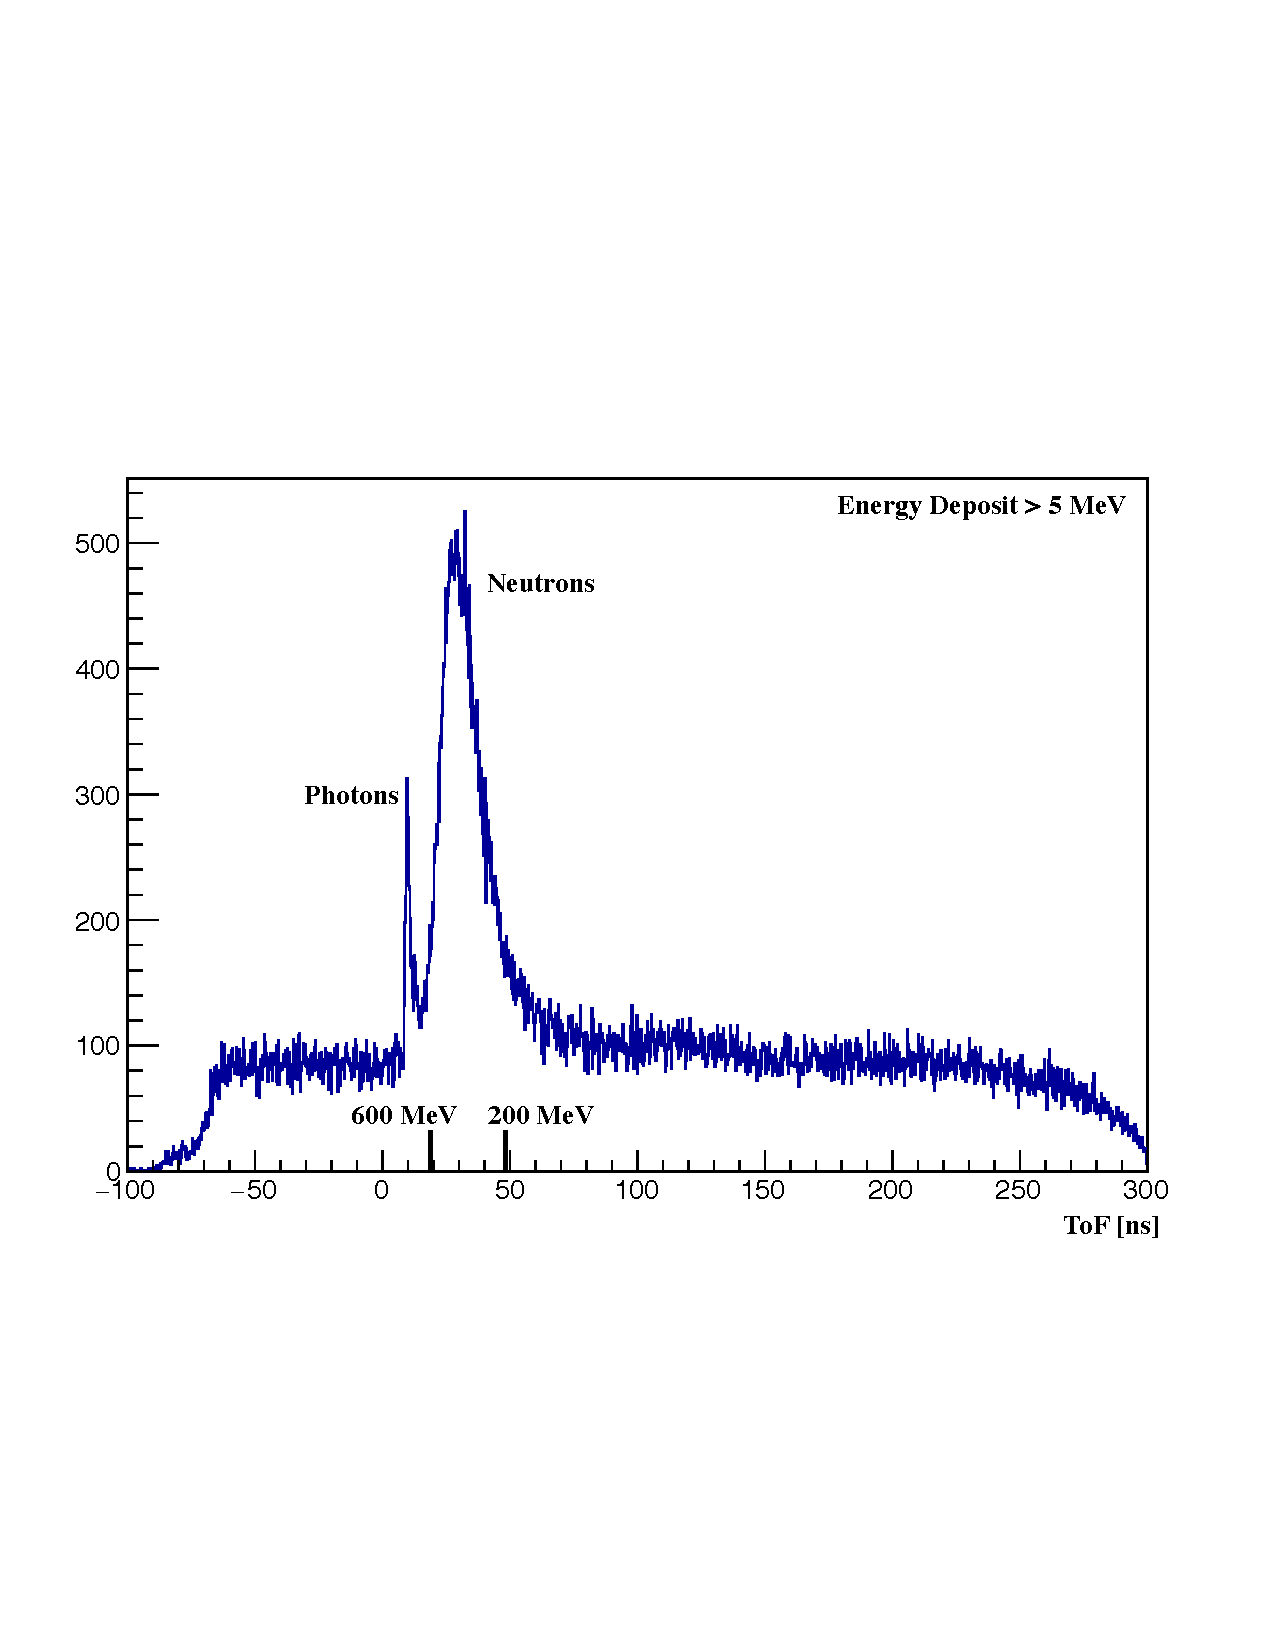
\includegraphics[width=0.96\textwidth]{tof-labels.pdf}
\caption{}
\end{figure}


% ==================================================================================================
\subsection{Magnetic testing}

% ---------------------------------------------------
\begin{figure}[h!]
\centering
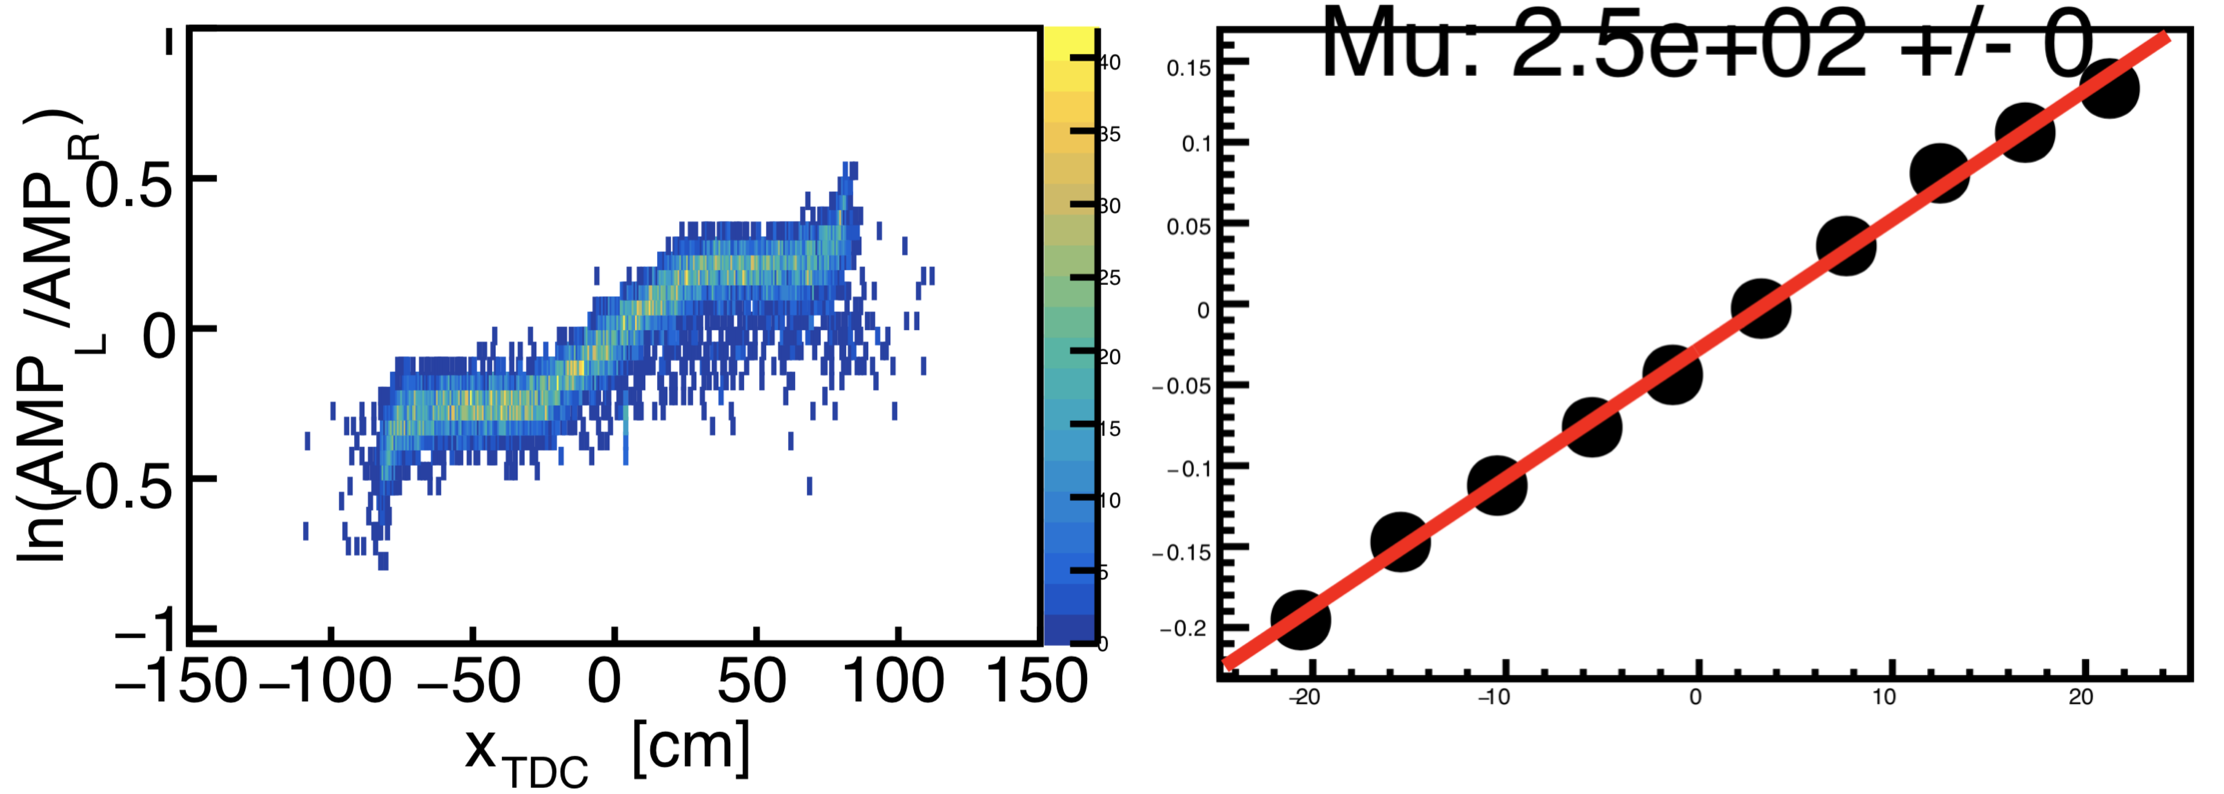
\includegraphics[width=0.96\textwidth]{atten.png}
\caption{}
\end{figure}
% ---------------------------------------------------

% ==================================================================================================
\subsection{Resolution}

% ---------------------------------------------------
\begin{figure}[h!]
\centering
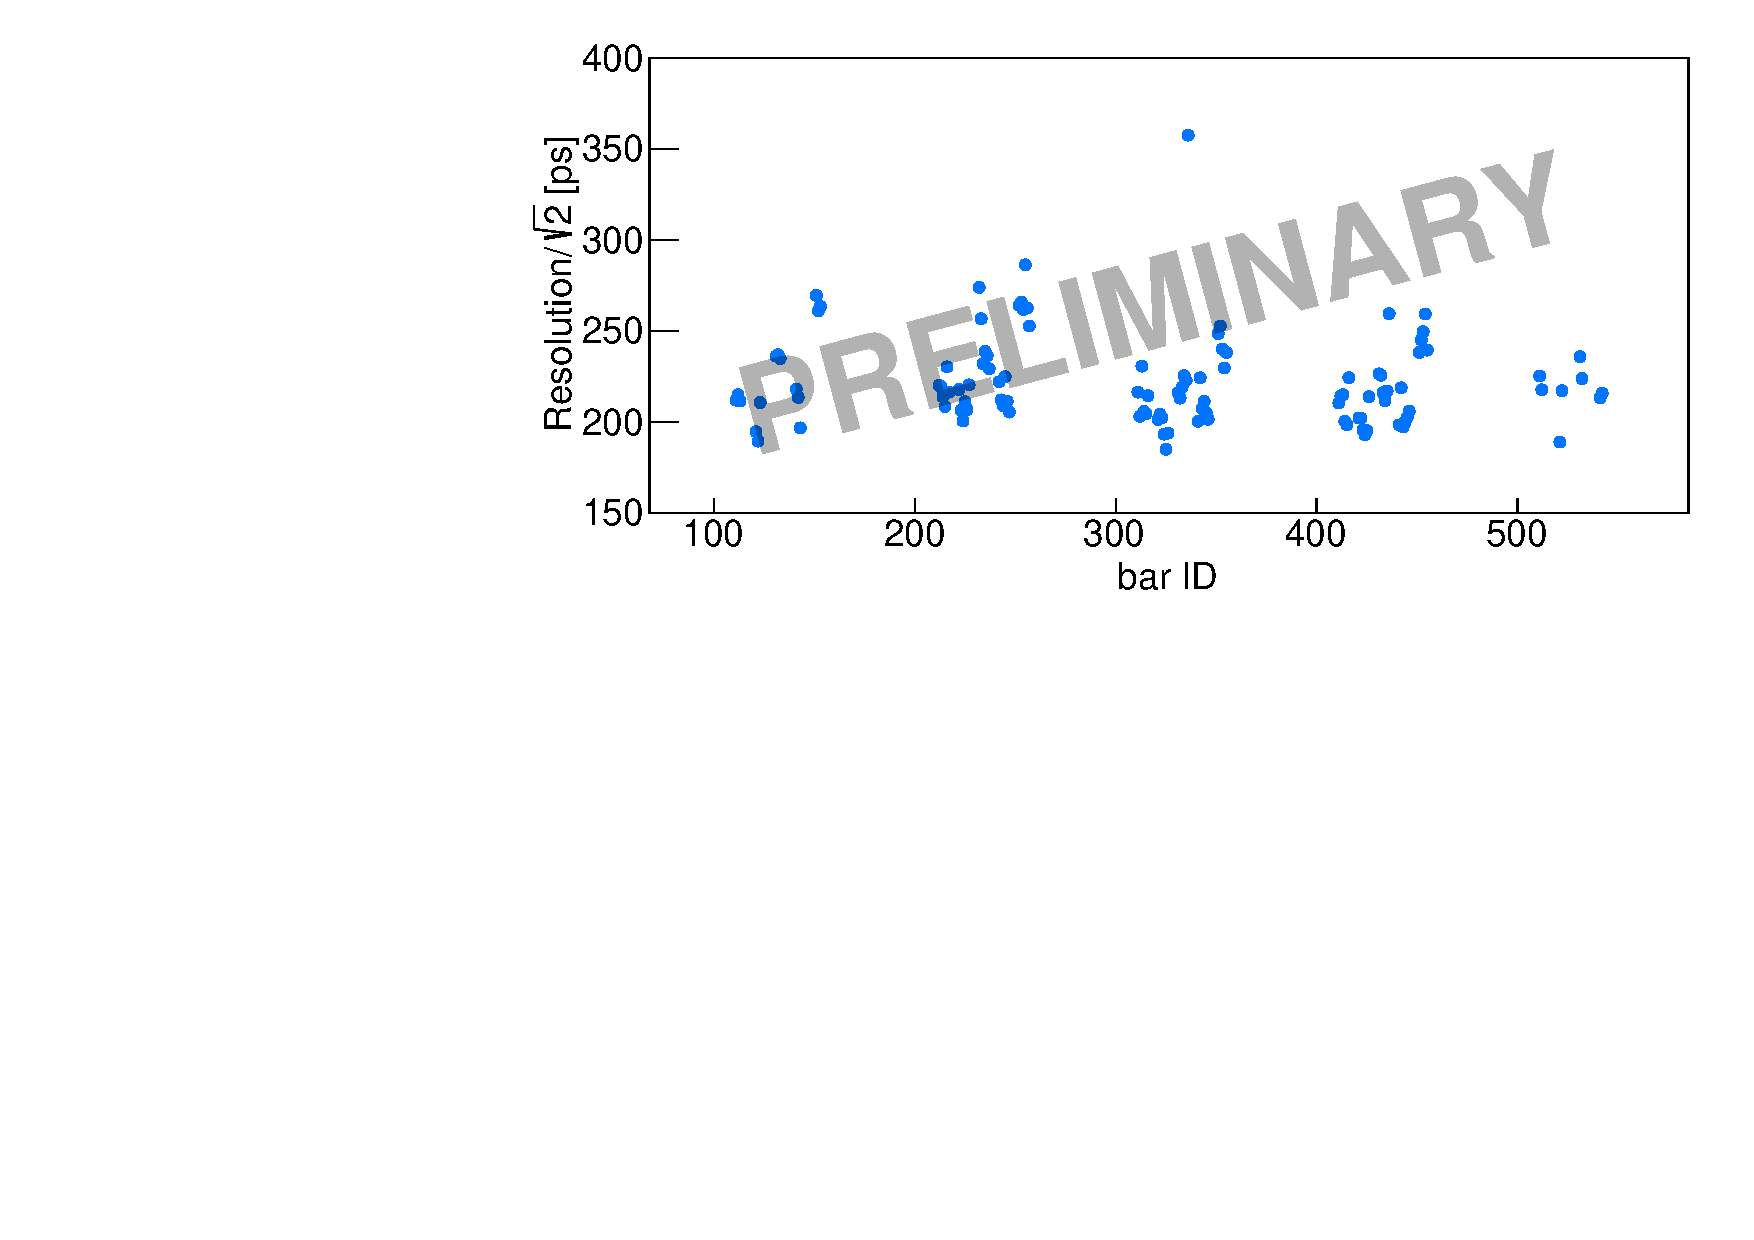
\includegraphics[width=0.8\textwidth]{figures/calibrations/resolutions.pdf}
\caption{}
\end{figure}
% ---------------------------------------------------

\fi

%%%%%%%%%%%%%%%%%%%%%%%%%%%%%%%%%%%%%%%%%%%%%%%%%%%%%%%%%%%%%%%%%%%%%%%%%%%%%%%%%%%%%%%%%%%%%%%%%%%

\section{Summary}

%%%%%%%%%%%%%%%%%%%%%%%%%%%%%%%%%%%%%%%%%%%%%%%%%%%%%%%%%%%%%%%%%%%%%%%%%%%%%%%%%%%%%%%%%%%%%%%%%%%

\section{Acknowledgements}

%%%%%%%%%%%%%%%%%%%%%%%%%%%%%%%%%%%%%%%%%%%%%%%%%%%%%%%%%%%%%%%%%%%%%%%%%%%%%%%%%%%%%%%%%%%%%%%%%%%

\section*{References}

% Create the reference section using BibTeX:
\bibliography{band_nim_bib}


\end{document}